%----------------------------------------------------------------------------------------
%	PACKAGES AND OTHER DOCUMENT CONFIGURATIONS
%----------------------------------------------------------------------------------------

\documentclass[11pt,fleqn]{book} % Default font size and left-justified equations

\usepackage[top=3cm,bottom=3cm,left=3.2cm,right=3.2cm,headsep=10pt,letterpaper]{geometry} % Page margins
\usepackage{xcolor} % Required for specifying colors by name
\definecolor{ocre}{RGB}{52,177,201} % Define the orange color used for highlighting throughout the book
\usepackage[section]{placeins}
% Font Settings
%\usepackage{avant} % Use the Avantgarde font for headings
%\usepackage{times} % Use the Times font for headings
%\usepackage{mathptmx} % Use the Adobe Times Roman as the default text font together with math symbols from the Sym­bol, Chancery and Com­pr Modern fonts

\usepackage{microtype} % Slightly tweak font spacing for aesthetics
\usepackage[utf8]{inputenc} % Required for including letters with accents
\usepackage[T1]{fontenc} % Use 8-bit encoding that has 256 glyphs

\usepackage{textgreek}
\usepackage{caption}
\usepackage{subcaption}
\usepackage[fulldiodes,siunitx, nooldvoltagedirection]{circuitikz}
\usepackage{csquotes}
\usepackage{siunitx}

% Bibliography
\usepackage[
backend=biber,
style=alphabetic,
sorting=ynt
]{biblatex}
\addbibresource{bibliography.bib}

\usepackage{makeidx}\makeindex 
%%%%%%%%%%%%%%%%%%%%%%%%%%%%%%%%%%%%%%%%%
% This is based on the Legrand Orange Book
% Structural Definitions File
%
% The original template (the Legrand Orange Book Template) can be found here --> http://www.latextemplates.com/template/the-legrand-orange-book
%
% Original author of the Legrand Orange Book Template::
% Mathias Legrand (legrand.mathias@gmail.com) with modifications by:
% Vel (vel@latextemplates.com)
%
% Original License:
% CC BY-NC-SA 3.0 (http://creativecommons.org/licenses/by-nc-sa/3.0/)
%
%%%%%%%%%%%%%%%%%%%%%%%%%%%%%%%%%%%%%%%%%
%----------------------------------------------------------------------------------------
%	VARIOUS REQUIRED PACKAGES
%----------------------------------------------------------------------------------------

\usepackage{titlesec} % Allows customization of titles

\usepackage{graphicx} % Required for including pictures
\graphicspath{{Pictures/}} % Specifies the directory where pictures are stored

\usepackage{lipsum} % Inserts dummy text

\usepackage{tikz} % Required for drawing custom shapes

\usepackage[english]{babel} % English language/hyphenation

\usepackage{enumitem} % Customize lists
\setlist{nolistsep} % Reduce spacing between bullet points and numbered lists

\usepackage{booktabs} % Required for nicer horizontal rules in tables

\usepackage{eso-pic} % Required for specifying an image background in the title page

%----------------------------------------------------------------------------------------
%	MAIN TABLE OF CONTENTS
%----------------------------------------------------------------------------------------

\usepackage{titletoc} % Required for manipulating the table of contents

\contentsmargin{0cm} % Removes the default margin
% Chapter text styling
\titlecontents{chapter}[1.25cm] % Indentation
{\addvspace{15pt}\large\sffamily\bfseries} % Spacing and font options for chapters
{\color{ocre!60}\contentslabel[\Large\thecontentslabel]{1.25cm}\color{ocre}} % Chapter number
{}  
{\color{ocre!60}\normalsize\sffamily\bfseries\;\titlerule*[.5pc]{.}\;\thecontentspage} % Page number
% Section text styling
\titlecontents{section}[1.25cm] % Indentation
{\addvspace{5pt}\sffamily\bfseries} % Spacing and font options for sections
{\contentslabel[\thecontentslabel]{1.25cm}} % Section number
{}
{\sffamily\hfill\color{black}\thecontentspage} % Page number
[]
% Subsection text styling
\titlecontents{subsection}[1.25cm] % Indentation
{\addvspace{1pt}\sffamily\small} % Spacing and font options for subsections
{\contentslabel[\thecontentslabel]{1.25cm}} % Subsection number
{}
{\sffamily\;\titlerule*[.5pc]{.}\;\thecontentspage} % Page number
[] 

%----------------------------------------------------------------------------------------
%	MINI TABLE OF CONTENTS IN CHAPTER HEADS
%----------------------------------------------------------------------------------------

% Section text styling
\titlecontents{lsection}[0em] % Indendating
{\footnotesize\sffamily} % Font settings
{}
{}
{}

% Subsection text styling
\titlecontents{lsubsection}[.5em] % Indentation
{\normalfont\footnotesize\sffamily} % Font settings
{}
{}
{}
 
%----------------------------------------------------------------------------------------
%	PAGE HEADERS
%----------------------------------------------------------------------------------------

\usepackage{fancyhdr} % Required for header and footer configuration

\pagestyle{fancy}
\renewcommand{\chaptermark}[1]{\markboth{\sffamily\normalsize\bfseries\chaptername\ \thechapter.\ #1}{}} % Chapter text font settings
\renewcommand{\sectionmark}[1]{\markright{\sffamily\normalsize\thesection\hspace{5pt}#1}{}} % Section text font settings
\fancyhf{} \fancyhead[LE,RO]{\sffamily\normalsize\thepage} % Font setting for the page number in the header
\fancyhead[LO]{\rightmark} % Print the nearest section name on the left side of odd pages
\fancyhead[RE]{\leftmark} % Print the current chapter name on the right side of even pages
\renewcommand{\headrulewidth}{0.5pt} % Width of the rule under the header
\addtolength{\headheight}{2.5pt} % Increase the spacing around the header slightly
\renewcommand{\footrulewidth}{0pt} % Removes the rule in the footer
\fancypagestyle{plain}{\fancyhead{}\renewcommand{\headrulewidth}{0pt}} % Style for when a plain pagestyle is specified

% Removes the header from odd empty pages at the end of chapters
\makeatletter
\renewcommand{\cleardoublepage}{
\clearpage\ifodd\c@page\else
\hbox{}
\vspace*{\fill}
\thispagestyle{empty}
\newpage
\fi}

%----------------------------------------------------------------------------------------
%	THEOREM STYLES
%----------------------------------------------------------------------------------------

\usepackage{amsmath,amsfonts,amssymb,amsthm} % For math equations, theorems, symbols, etc
\let\Bbbk\relax
\usepackage{txfonts}
\newcommand{\intoo}[2]{\mathopen{]}#1\,;#2\mathclose{[}}
\newcommand{\ud}{\mathop{\mathrm{{}d}}\mathopen{}}
\newcommand{\intff}[2]{\mathopen{[}#1\,;#2\mathclose{]}}
\newtheorem{notation}{Notation}[chapter]

%%%%%%%%%%%%%%%%%%%%%%%%%%%%%%%%%%%%%%%%%%%%%%%%%%%%%%%%%%%%%%%%%%%%%%%%%%%
%%%%%%%%%%%%%%%%%%%% dedicated to boxed/framed environements %%%%%%%%%%%%%%
%%%%%%%%%%%%%%%%%%%%%%%%%%%%%%%%%%%%%%%%%%%%%%%%%%%%%%%%%%%%%%%%%%%%%%%%%%%
\newtheoremstyle{ocrenumbox}% % Theorem style name
{0pt}% Space above
{0pt}% Space below
{\normalfont}% % Body font
{}% Indent amount
{\small\bf\sffamily\color{ocre}}% % Theorem head font
{\;}% Punctuation after theorem head
{0.25em}% Space after theorem head
{\small\sffamily\color{ocre}\thmname{#1}\nobreakspace\thmnumber{\@ifnotempty{#1}{}\@upn{#2}}% Theorem text (e.g. Theorem 2.1)
\thmnote{\nobreakspace\the\thm@notefont\sffamily\bfseries\color{black}---\nobreakspace#3.}} % Optional theorem note
\renewcommand{\qedsymbol}{$\blacksquare$}% Optional qed square

\newtheoremstyle{blacknumex}% Theorem style name
{5pt}% Space above
{5pt}% Space below
{\normalfont}% Body font
{} % Indent amount
{\small\bf\sffamily}% Theorem head font
{\;}% Punctuation after theorem head
{0.25em}% Space after theorem head
{\small\sffamily{\tiny\ensuremath{\blacksquare}}\nobreakspace\thmname{#1}\nobreakspace\thmnumber{\@ifnotempty{#1}{}\@upn{#2}}% Theorem text (e.g. Theorem 2.1)
\thmnote{\nobreakspace\the\thm@notefont\sffamily\bfseries---\nobreakspace#3.}}% Optional theorem note

\newtheoremstyle{blacknumbox} % Theorem style name
{0pt}% Space above
{0pt}% Space below
{\normalfont}% Body font
{}% Indent amount
{\small\bf\sffamily}% Theorem head font
{\;}% Punctuation after theorem head
{0.25em}% Space after theorem head
{\small\sffamily\thmname{#1}\nobreakspace\thmnumber{\@ifnotempty{#1}{}\@upn{#2}}% Theorem text (e.g. Theorem 2.1)
\thmnote{\nobreakspace\the\thm@notefont\sffamily\bfseries---\nobreakspace#3.}}% Optional theorem note

%%%%%%%%%%%%%%%%%%%%%%%%%%%%%%%%%%%%%%%%%%%%%%%%%%%%%%%%%%%%%%%%%%%%%%%%%%%
%%%%%%%%%%%%% dedicated to non-boxed/non-framed environements %%%%%%%%%%%%%
%%%%%%%%%%%%%%%%%%%%%%%%%%%%%%%%%%%%%%%%%%%%%%%%%%%%%%%%%%%%%%%%%%%%%%%%%%%
\newtheoremstyle{ocrenum}% % Theorem style name
{5pt}% Space above
{5pt}% Space below
{\normalfont}% % Body font
{}% Indent amount
{\small\bf\sffamily\color{ocre}}% % Theorem head font
{\;}% Punctuation after theorem head
{0.25em}% Space after theorem head
{\small\sffamily\color{ocre}\thmname{#1}\nobreakspace\thmnumber{\@ifnotempty{#1}{}\@upn{#2}}% Theorem text (e.g. Theorem 2.1)
\thmnote{\nobreakspace\the\thm@notefont\sffamily\bfseries\color{black}---\nobreakspace#3.}} % Optional theorem note
\renewcommand{\qedsymbol}{$\blacksquare$}% Optional qed square
\makeatother

% Defines the theorem text style for each type of theorem to one of the three styles above
\newcounter{dummy} 
\numberwithin{dummy}{section}
\theoremstyle{ocrenumbox}
\newtheorem{theoremeT}[dummy]{Theorem}
\newtheorem{problem}{Problem}[chapter]
\newtheorem{exerciseT}{Exercise}[chapter]
\theoremstyle{blacknumex}
\newtheorem{exampleT}{Example}[chapter]
\theoremstyle{blacknumbox}
\newtheorem{vocabulary}{Vocabulary}[chapter]
\newtheorem{definitionT}{Definition}[section]
\newtheorem{corollaryT}[dummy]{Corollary}
\theoremstyle{ocrenum}
\newtheorem{proposition}[dummy]{Proposition}

%----------------------------------------------------------------------------------------
%	DEFINITION OF COLORED BOXES
%----------------------------------------------------------------------------------------

\RequirePackage[framemethod=default]{mdframed} % Required for creating the theorem, definition, exercise and corollary boxes

% Theorem box
\newmdenv[skipabove=7pt,
skipbelow=7pt,
backgroundcolor=black!5,
linecolor=ocre,
innerleftmargin=5pt,
innerrightmargin=5pt,
innertopmargin=5pt,
leftmargin=0cm,
rightmargin=0cm,
innerbottommargin=5pt]{tBox}

% Exercise box	  
\newmdenv[skipabove=7pt,
skipbelow=7pt,
rightline=false,
leftline=true,
topline=false,
bottomline=false,
backgroundcolor=ocre!10,
linecolor=ocre,
innerleftmargin=5pt,
innerrightmargin=5pt,
innertopmargin=5pt,
innerbottommargin=5pt,
leftmargin=0cm,
rightmargin=0cm,
linewidth=4pt]{eBox}	

% Definition box
\newmdenv[skipabove=7pt,
skipbelow=7pt,
rightline=false,
leftline=true,
topline=false,
bottomline=false,
linecolor=ocre,
innerleftmargin=5pt,
innerrightmargin=5pt,
innertopmargin=0pt,
leftmargin=0cm,
rightmargin=0cm,
linewidth=4pt,
innerbottommargin=0pt]{dBox}	

% Corollary box
\newmdenv[skipabove=7pt,
skipbelow=7pt,
rightline=false,
leftline=true,
topline=false,
bottomline=false,
linecolor=gray,
backgroundcolor=black!5,
innerleftmargin=5pt,
innerrightmargin=5pt,
innertopmargin=5pt,
leftmargin=0cm,
rightmargin=0cm,
linewidth=4pt,
innerbottommargin=5pt]{cBox}

% Creates an environment for each type of theorem and assigns it a theorem text style from the "Theorem Styles" section above and a colored box from above
\newenvironment{theorem}{\begin{tBox}\begin{theoremeT}}{\end{theoremeT}\end{tBox}}
\newenvironment{exercise}{\begin{eBox}\begin{exerciseT}}{\hfill{\color{ocre}\tiny\ensuremath{\blacksquare}}\end{exerciseT}\end{eBox}}				  
\newenvironment{definition}{\begin{dBox}\begin{definitionT}}{\end{definitionT}\end{dBox}}	
\newenvironment{example}{\begin{exampleT}}{\hfill{\tiny\ensuremath{\blacksquare}}\end{exampleT}}		
\newenvironment{corollary}{\begin{cBox}\begin{corollaryT}}{\end{corollaryT}\end{cBox}}	

%----------------------------------------------------------------------------------------
%	REMARK ENVIRONMENT
%----------------------------------------------------------------------------------------

\newenvironment{remark}{\par\vspace{10pt}\small % Vertical white space above the remark and smaller font size
\begin{list}{}{
\leftmargin=35pt % Indentation on the left
\rightmargin=25pt}\item\ignorespaces % Indentation on the right
\makebox[-2.5pt]{\begin{tikzpicture}[overlay]
\node[draw=ocre!60,line width=1pt,circle,fill=ocre!25,font=\sffamily\bfseries,inner sep=2pt,outer sep=0pt] at (-15pt,0pt){\textcolor{ocre}{R}};\end{tikzpicture}} % Orange R in a circle
\advance\baselineskip -1pt}{\end{list}\vskip5pt} % Tighter line spacing and white space after remark

%----------------------------------------------------------------------------------------
%	SECTION NUMBERING IN THE MARGIN
%----------------------------------------------------------------------------------------

\makeatletter
\renewcommand{\@seccntformat}[1]{\llap{\textcolor{ocre}{\csname the#1\endcsname}\hspace{1em}}}                    
\renewcommand{\section}{\@startsection{section}{1}{\z@}
{-4ex \@plus -1ex \@minus -.4ex}
{1ex \@plus.2ex }
{\normalfont\large\sffamily\bfseries}}
\renewcommand{\subsection}{\@startsection {subsection}{2}{\z@}
{-3ex \@plus -0.1ex \@minus -.4ex}
{0.5ex \@plus.2ex }
{\normalfont\sffamily\bfseries}}
\renewcommand{\subsubsection}{\@startsection {subsubsection}{3}{\z@}
{-2ex \@plus -0.1ex \@minus -.2ex}
{.2ex \@plus.2ex }
{\normalfont\small\sffamily\bfseries}}                        
\renewcommand\paragraph{\@startsection{paragraph}{4}{\z@}
{-2ex \@plus-.2ex \@minus .2ex}
{.1ex}
{\normalfont\small\sffamily\bfseries}}

%----------------------------------------------------------------------------------------
%	HYPERLINKS IN THE DOCUMENTS
%----------------------------------------------------------------------------------------

% For an unclear reason, the package should be loaded now and not later
\usepackage{hyperref}
\hypersetup{hidelinks,colorlinks=false,breaklinks=true,urlcolor= ocre,pdftitle={Title},pdfauthor={Author}}
%backref=true,pagebackref=true,hyperindex=true,bookmarksopen=false,bookmarks=true
%----------------------------------------------------------------------------------------
%	CHAPTER HEADINGS
%----------------------------------------------------------------------------------------

% The set-up below should be (sadly) manually adapted to the overall margin page septup controlled by the geometry package loaded in the main.tex document. It is possible to implement below the dimensions used in the goemetry package (top,bottom,left,right)... TO BE DONE

\newcommand{\thechapterimage}{}
\newcommand{\chapterimage}[1]{\renewcommand{\thechapterimage}{#1}}

% Numbered chapters with mini tableofcontents
\def\thechapter{\arabic{chapter}}
\def\@makechapterhead#1{
\thispagestyle{empty}
{\centering \normalfont\sffamily
\ifnum \c@secnumdepth >\m@ne
\if@mainmatter
\startcontents
\begin{tikzpicture}[remember picture,overlay]
\node at (current page.north west)
{\begin{tikzpicture}[remember picture,overlay]
\node[anchor=north west,inner sep=0pt] at (0,0) {\includegraphics[width=\paperwidth]{\thechapterimage}};
%%%%%%%%%%%%%%%%%%%%%%%%%%%%%%%%%%%%%%%%%%%%%%%%%%%%%%%%%%%%%%%%%%%%%%%%%%%%%%%%%%%%%
% Commenting the 3 lines below removes the small contents box in the chapter heading
%\fill[color=ocre!10!white,opacity=.6] (1cm,0) rectangle (8cm,-7cm);
%\node[anchor=north west] at (1.1cm,.35cm) {\parbox[t][8cm][t]{6.5cm}{\huge\bfseries\flushleft \printcontents{l}{1}{\setcounter{tocdepth}{2}}}};
\draw[anchor=west] (8cm,-7cm) node []{\Huge\sffamily\bfseries\textcolor{black}{\thechapter. #1\strut\makebox[20cm]{}}};
%%%%%%%%%%%%%%%%%%%%%%%%%%%%%%%%%%%%%%%%%%%%%%%%%%%%%%%%%%%%%%%%%%%%%%%%%%%%%%%%%%%%%
\end{tikzpicture}};
\end{tikzpicture}}
\par\vspace*{230\p@}
\fi
\fi}

% Unnumbered chapters without mini tableofcontents (could be added though) 
\def\@makeschapterhead#1{
\thispagestyle{empty}
{\centering \normalfont\sffamily
\ifnum \c@secnumdepth >\m@ne
\if@mainmatter
\begin{tikzpicture}[remember picture,overlay]
\node at (current page.north west)
{\begin{tikzpicture}[remember picture,overlay]
\node[anchor=north west,inner sep=0pt] at (0,0) {\includegraphics[width=\paperwidth]{\thechapterimage}};
\draw[anchor=west] (8cm,-7cm) node []{\huge\sffamily\bfseries\textcolor{black}{#1\strut\makebox[22cm]{}}};
\end{tikzpicture}};
\end{tikzpicture}}
\par\vspace*{230\p@}
\fi
\fi
}
\makeatother % Insert the commands.tex file which contains the majority of the structure behind the template

\begin{document}
\def\TIMER555(#1)#2{%
  \begin{scope}[shift={(#1)}]
    \draw[fill=blue!10] (-1.5,-2) rectangle (1.5,2); % The body of IC
    % Label and component identifier.
    \draw[blue] (2,2.5) node []{\large \bf IC - #2}; % IC LABEL
    \draw[blue] (0,0.5) node [align=center]{\large NE-555\\TIMER}; % IC LABEL
    % Draw the pins
    % Some that you have to learn about label nodes, draw lines, and name coordinates in Tikz
    \draw (0.9,-2) node [above]{GND} -- +(0,-0.5) node [anchor=-45]{1} coordinate (#2 GND); % Pin 1 GND
    \draw (-1.5,-1.5) node [right]{TRG} -- +(-0.5,0) node [anchor=-135]{2} coordinate (#2 TRG); % Pin 2 TRG
    \draw (1.5,0) node [left]{OUT} -- +(0.5,0) node [anchor=-45]{3} coordinate (#2 OUT); % Pin 3 OUT  
    \draw (0.9,2) node [below]{RESET} -- +(0,0.5) node [anchor=45]{4} coordinate (#2 RESET); % Pin 4 RESET
    \draw (0,-2) node [above]{CTRL} -- +(0,-0.5) node [anchor=-45]{5} coordinate (#2 CTRL); % Pin 5 CTRL
    \draw (-1.5,-.5) node [right]{THR} -- +(-0.5,0) node [anchor=-135]{6} coordinate (#2 THR); % Pin 6 THR
    \draw (-1.5,1.5) node [right]{DIS} -- +(-0.5,0) node [anchor=-135]{7} coordinate (#2 DIS); % Pin 7 DIS
    \draw (0,2) node [below]{$\mathsf{V_{CC}}$} -- +(0,0.5) node [anchor=45]{8} coordinate (#2 VCC); % Pin 8 VCC
  \end{scope}
}

\tikzset{flipflop sr-rst/.style={flipflop,
    flipflop def={t1=S, t3=R, t6=Q, n6=1, nu=1},
}}
\title{Clustering the interstellar medium}

%----------------------------------------------------------------------------------------
%	TITLE PAGE
%----------------------------------------------------------------------------------------

\begingroup
\thispagestyle{empty}
\AddToShipoutPicture*{\put(0,0){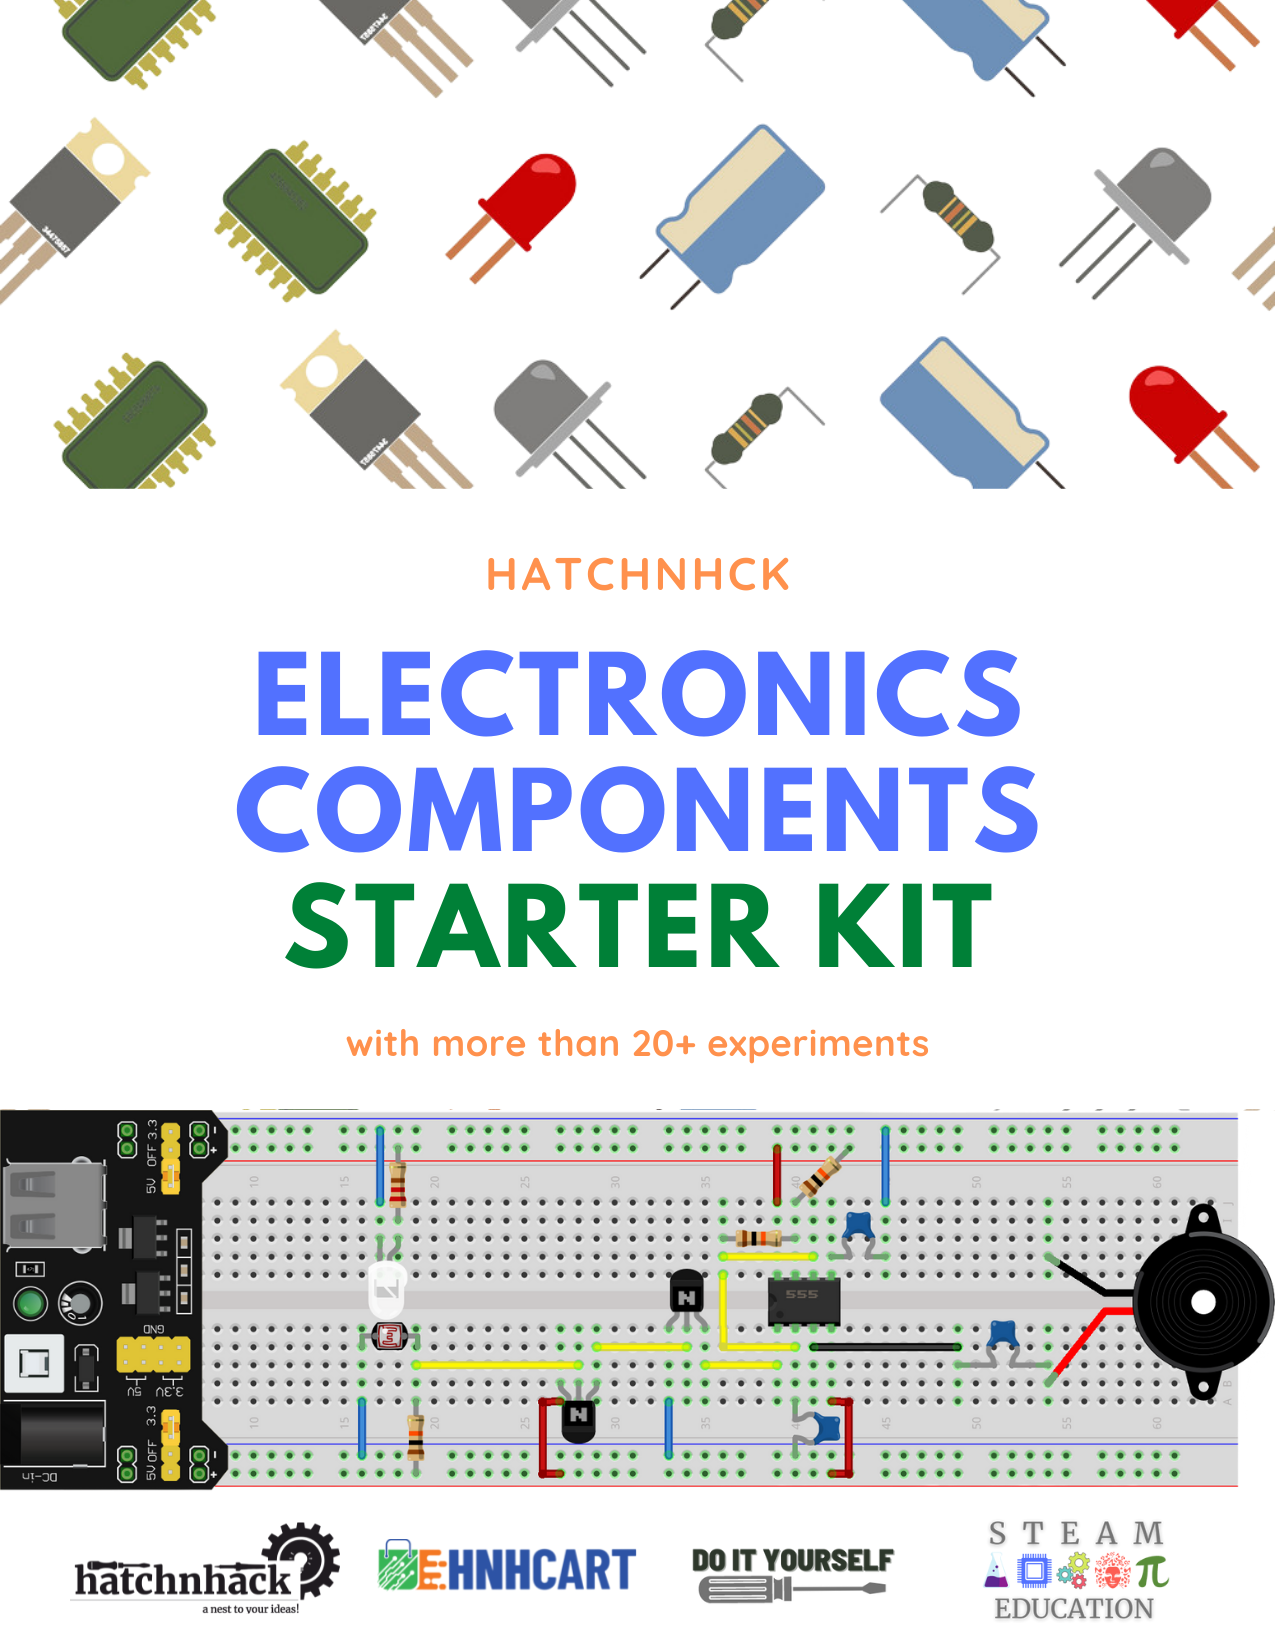
\includegraphics[width=\paperwidth]{esk_book_cover.png}}} % Image background
\centering
\vspace*{5cm}
\par\normalfont\fontsize{35}{35}\sffamily\selectfont
%\textbf{Electronics Starter Kit}\\
%{\LARGE Learn | Experiment | Fun}\par % Book title
\vspace*{1cm}
%{\Huge HatchnHack}\par % Author name
\endgroup

%----------------------------------------------------------------------------------------
%	COPYRIGHT PAGE
%----------------------------------------------------------------------------------------

\newpage
~\vfill
\thispagestyle{empty}

%\noindent Copyright \copyright\ 2014 Andrea Hidalgo\\ % Copyright notice

\noindent \textsc{HatchnHack - A nest to your ideas}\\

\noindent \textsc{https://github.com/hatchnhack/Electronics-Starter-Kit}\\ % URL

\noindent \textit{First release, September 2020} % Printing/edition date

%----------------------------------------------------------------------------------------
%	TABLE OF CONTENTS
%----------------------------------------------------------------------------------------

\chapterimage{head1.png} % Table of contents heading image

\pagestyle{empty} % No headers

\tableofcontents % Print the table of contents itself

%\cleardoublepage % Forces the first chapter to start on an odd page so it's on the right

\pagestyle{fancy} % Print headers again

%-------------------
% Sections
% - LED
% - Transistor
% - 555
% - Motor
%-------------------

%----------------------------------------------------------------------------------------
%	CHAPTER 1
%----------------------------------------------------------------------------------------

\chapterimage{head2.png} % Chapter heading image

\chapter{Introduction}

\begin{quote}
    Creating means living - Dejan Stojanovic
\end{quote}
This guide will guide you to make smart circuits or systems using discrete components like transistors, resistors, LEDs, NE555 timer IC, without micro-controllers or programming.
In the following section, all the kits components' working and uses are explained thoroughly, and after that each chapter is divided according to the experiments and components. You can directly build the circuit you like or go through this guide to get an in-depth knowledge of every component and system and customize them to make your own circuits.

\section{Kit Introduction}\index{Kit Introduction}
In this section all the electronic components that you have received in the kits are explained with example circuits and use case.

The list of components in the kits - 
\begin{itemize}
\item Battery
\item Battery Connector
\item Jumper Wires
\item Male Headers
\item Breadboard
\item Resistor Box
\item Ceramic Capacitor
\item Potentiometer
\item Potentiometer Knob
\item LDR
\item Push Button
\item Diode
\item LED
\item Transistor
\item Power Supply Module
\item Buzzer
\item NE555 IC
\item Toy Motor
\item Toy Fan
\end{itemize}

\section{Components' Introduction}\index{Components' Introduction}

\subsection{Battery}
%----------------------------------------------------------------------------------------
%	CHAPTER 2
%----------------------------------------------------------------------------------------
%\chapterimage{}

\chapter{Fun with LEDs}

\section{Overview}\index{Overview}
In this section you'll learn about Light Emitting Diodes (LED) and how to turn it on using different methods.


\section{Component Introduction}\index{Component Introduction!LEDs}
Before diving into making circuits, we will first learn about the components that we are going to use and how to select the right component.

\subsection{Resistors}
Resistor is a passive electric component that resists the flow of current through it. They are used in almost all electrical and electronic circuits and systems. The resistance of a resistor in measured in ohms (\textOmega).
An ohm is the resistance that occurs when one ampere (A) of current flows through a resistor with potential (or voltage) drop of one volt (V) across it's terminal.
\begin{figure}[htp]
    \centering
    \begin{circuitikz}[scale = 2]
        \draw[very thick] (0,0) to[resistor, color = red] (2,0);
    \end{circuitikz}
    \caption{Resistor Symbol}
    \label{fig:resistor_symbol}
\end{figure}

\subsubsection{Ohm's Law}
Ohm's law state that the current through a resistor is directly proportional to the voltage applied across it.
\begin{align*}
    I \propto V \\
    \Longrightarrow
    R = \frac{V}{I} (\Omega)
\end{align*}

\subsection{Light Emitting Diode}
Light emitting diodes (LEDs) are semiconductor devices that emit lights of different wavelength depending on the substrate semiconductor material used when an electric current is applied. The color of light emitted depends on the amount of energy required by the electrons to cross the band gap of the semiconductor. Since, LEDs are basically a PN junction diode, they allow current flow only in one direction.

\begin{figure}[htp]
    \centering
    \begin{circuitikz}[scale = 2]
        \draw[very thick] (0,0) to[full led, color = red] (2,0);
    \end{circuitikz}
    \caption{LED Symbol}
    \label{fig:led_symbol}
\end{figure}

\subsubsection{Determining the pins of the LED}
There are multiple ways to determine the anode and cathode of an LED:
\begin{enumerate}
    \item Looking at the LED pins (or legs). The longer leg is anode and the shorter cathode. But sometimes the legs could be trimmed, therefore, you can use this method for new LEDs only.
    \item Locate a flat edge on the LED. The pin close to flat edge is cathode.
    \item By looking inside the LED, the bigger conductor (flag shaped) is the cathode.
    \item By using multi-meter in continuity mode, only is one direction the LED will turn on (or the resistance in one direction will be smaller than in the other).
\end{enumerate}

\subsection{Breadboard}
A breadboard in a rectangular plastic board with a bunch of tiny holes in it. There's strip of metal inside the plastic. Most through hole components have pin spacing of 2.54mm, therefore, the holes have the same spacing between them. You can easily insert electrical components in these holes. There is also a deep grove in the middle, indicating the break in the connection. Some breadboard have two strips of holes (also called rails) along the long edges of the breadboard. They are used for power rails, with strip of metal inside.

A breadboard is used to prototype an electronic circuit. The connection on breadboard are not permanent and can be removed easily. This makes breadboard great for beginners who are new to electronics but the connections are not as reliable as soldered connections.

\subsection{Breadboard Power Supply}
A power supply is a hardware component that provides electricity to power devices like computer, fridge, lights and much more. The breadboard power supply of type linear DC to DC. A linear power supply has two major components, a linear regulator and filtering capacitors.

The breadboard power supply can provide constant 3.3V or 5V and is compatible with the breadboard power rails, i.e., you can directly plug in on top of the breadboard to have voltage across the power rails.
The input voltage or power can be provided through the DC barrel jack (for 6-12V) or through the USB connector (5V).

\begin{figure}[htp]
    \centering
    \begin{circuitikz}[scale = 2]
        \draw
            [very thick] (0,2) to[battery, color = red] (0,0)
            (0.2,1.2) node{$+$}
            (0.2,0.8) node{$-$};
    \end{circuitikz}
    \caption{Battery Symbol}
    \label{fig:battery_symbol}
\end{figure}

\subsubsection{Calculating power dissipation}
To calculate the power dissipation across the voltage regulator, we need to determine the output current. For linear regulator the input and output current remains same and the power difference is dissipated through the voltage regulator.

Example: We need 200mA current at 3,3V output, and the input power supply is of 9V. Then,
\begin{align*}
    P_{out} &= 3.3V \times 0.2A = 0.66W \\
    P_{in} &= 9V \times 0.2A = 1.8W \\
    P_{reg} &= P_{in} - P_{out} \\
        &= 1.8 - 0.66 \\
        &= 1.14W \\
    \eta &= \frac{P_{out}}{P_{in}} \times 100\\
        &= 36.67 \%
\end{align*}

\subsection{Push Button}
Push button is use to control or provide input to the circuit. It is normally open and only when you press it the current will flow through it. And when released, the current will stop flowing. Push button have mechanical contacts, so when you press or release it, it doesn't instantaneously make or release contact. It bounces back and forth before making a firm connection.
\begin{figure}[htp]
    \centering
    \begin{circuitikz}[scale = 2]
        \draw[very thick] (0,0) to[push button, color = red] (2,0);
    \end{circuitikz}
    \caption{Push Button Symbol}
    \label{fig:pb_symbol}
\end{figure}

\subsection{Potentiometer}
A potentiometer (pot) is a variable resistor and comes in different packages, size and values. They generally have 3 terminals. And the resistance between the outer most terminals is equal to the maximum resistance of the potentiometer and the resistance between middle and any outer pin can vary from 0 to the total resistance of potentiometer.
\begin{figure}[htp]
    \centering
    \begin{circuitikz}[scale = 2]
        \draw[very thick] (0,0) to[american potentiometer, color = red] (2,0);
    \end{circuitikz}
    \caption{Potentiometer Symbol}
    \label{fig:pot_symbol}
\end{figure}

\subsection{Circuit}
A circuit is a closed loop that provides path for current to flow. Circuit must have a path that start and end at the same component, or in order words must form a loop. Electronic circuits operates at low voltages.
\begin{figure}[htp]
    \centering
    \begin{circuitikz}[scale = 2]
        \draw
            [blue] (0,0) to[short] (3,0)
            (0,1) to[full led, color=red] (3,1)
            (3,0) to[R] (3,1)
            (0,1) to[battery, color=red] (0,0);
    \end{circuitikz}
    \caption{Simple Circuit}
    \label{fig:simple_circuit}
\end{figure}

A circuit has broadly the following components -
\begin{itemize}
    \item Power source\/supply
    \item Load (Light, led, motor etc)
    \item Path\/wire (conductive path providing current flow)
\end{itemize}
Apart from these, a circuit can have more complex design.
\clearpage

% Lesson starts here
\section{Lesson 1: Lighting up an LED}\index{Lesson 1: Lighting up an LED}
\subsection{Objective}
In this activity you'll learn how to turn on an LED
\subsection{Components Required}
\begin{enumerate}
    \item Breadboard Power Supply $\times$ 1
    \item 9V Battery $\times$ 1 
    \item 9V Battery Connector $\times$ 1
    \item Breadboard $\times$ 1
    \item 5mm Red LED $\times$ 1
    \item 220$\Omega$ resistor $\times$ 1
    \item Male to Male Jumper Wires $\times$ 2
\end{enumerate}
\subsection{Circuit}
\begin{figure}[htp]
    \centering
    \begin{subfigure}[b]{0.4\textwidth}
        \centering
        \begin{circuitikz}[scale = 2]
            \draw[very thick]
                (0,0) to[short] (2,0)
                (0,1) to[full led, color=red] (2,1)
                (2,0) to[R, l^=$R_s (220\Omega)$] (2,1)
                (0,1) to[battery, color=red, l_=$5V$] (0,0);
        \end{circuitikz}
        \caption{Circuit A}
    \end{subfigure}
    \hfill
    \begin{subfigure}[b]{0.4\textwidth}
        \centering
        \begin{circuitikz}[scale = 2]
            \draw[very thick]
                (0,0) to[short] (2,0)
                (0,1) to[R, l^=$R_s (220\Omega)$] (2,1)
                (2,1) to[full led, color=red] (2,0)
                (0,1) to[battery, color=red, l_=$5V$] (0,0);
        \end{circuitikz}
        \caption{Circuit B}
    \end{subfigure}
    \caption{Simple LED Circuits}
    \label{fig:simple_led_circuit}
\end{figure}
Throughout this guide we'll be using these symbols for power supply.
\begin{figure}[htp]
    \centering
    \begin{subfigure}[b]{0.4\textwidth}
        \centering
        \begin{circuitikz}[scale = 2]
            \draw
                (0,1) to[empty led, color=red] (0,0)
                (0,0) node[ground] {}
                (0,1) to[R, l^=$R_s (220\Omega)$] (0,2)
                (-0.2,2) -- node[anchor=south] {5V} (0.2,2);
        \end{circuitikz}
        \caption{Circuit A}
    \end{subfigure}
    \hfill
    \begin{subfigure}[b]{0.4\textwidth}
        \centering
        \begin{circuitikz}[scale = 2]
            \draw
                (0,2) to[empty led, color=red] (0,1)
                (0,0) node[ground] {}
                (0,1) to[R, l^=$R_s (220\Omega)$] (0,0)
                (-0.2,2) -- node[anchor=south] {5V} (0.2,2);
        \end{circuitikz}
        \caption{Circuit B}
    \end{subfigure}
    \caption{Simplified LED Circuits}
    \label{fig:led_circuit}
\end{figure}
\subsection{Circuit Explanation}
If we look at the graphs in the datasheet of RED led\cite{tlur640}, the forward current through the led ($I_F$) is typically 
in between \SI{10}{mA} to \SI{20}{mA} and the voltage drop ($V_F$) across it is \SI{2}{V}. If we directly connect the LED across 
\SI{5}{V} supply it will burn out due to excessive power. Therefore, we need a resistor in series with the LED to drop the voltage. 
This resistor is referred as the current-limiting resistor. If you look at the figure \ref{fig:simple_led_circuit} both the circuits 
A \& B are same because in series circuits the current remains same across all the components.

To calculate the series resistance ($R_S$) we'll use Ohm's law:
We'll take the average value for $I_F$
\begin{align*}
    V &= I \times R \\
    R_S &= \frac{V_{5v} - V_F}{I_F} \\
        &= \frac{5V - 2V}{15mA} \\
        &= \frac{3 \times 1000}{15} \\
    R_S &= \SI{200}{\Omega}
\end{align*}
Since, in the kit a \SI{220}{\ohm} is available, we will use that. If we calculate the current using a \SI{220}{\ohm} resistor, it will $3 \div 220 = \SI{0.0136}{\ampere} = \SI{13.6}{\mA}$ which is in the range provided by the datasheet.
\subsection{Circuit Picture}
\begin{figure}[htp]
    \centering
    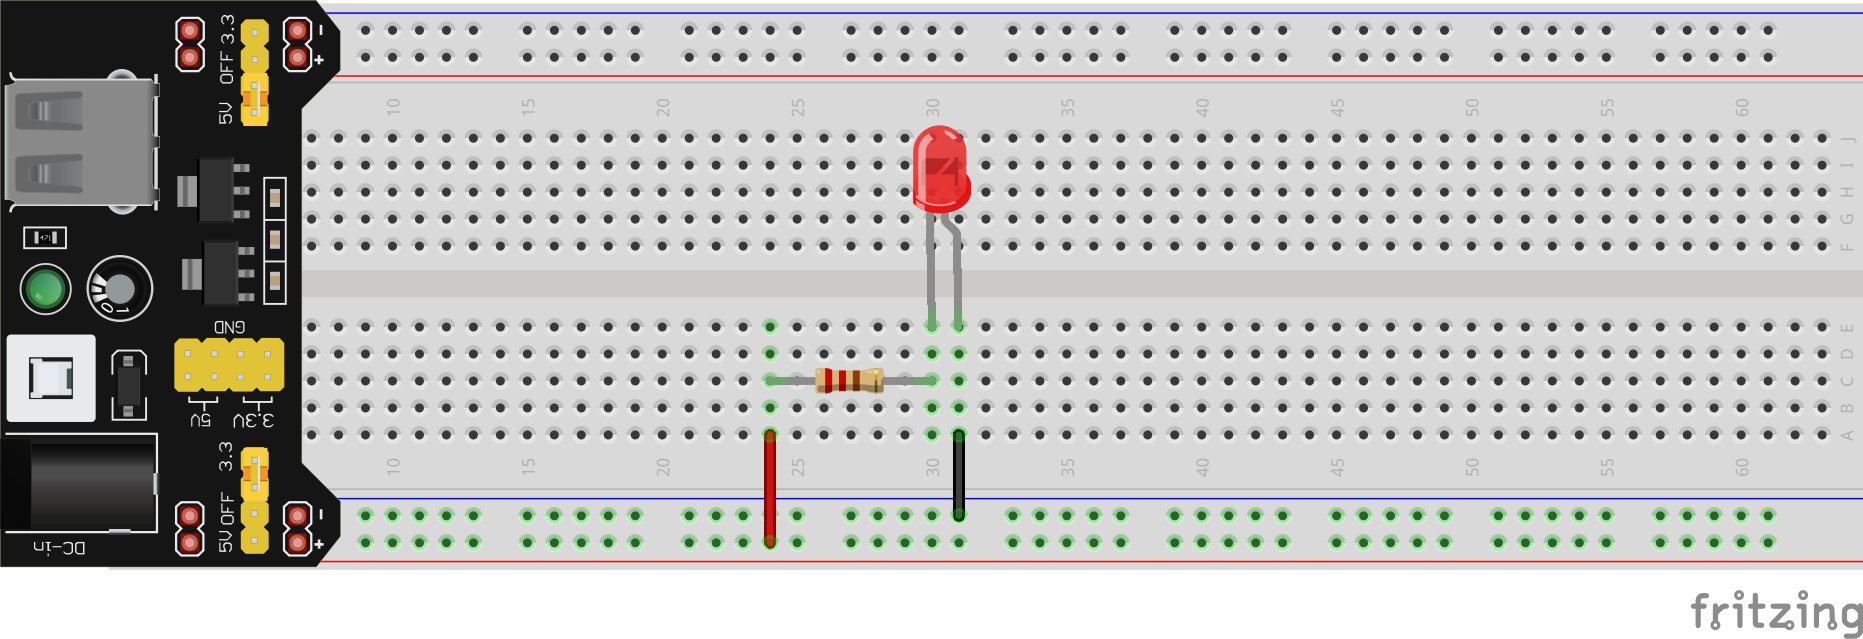
\includegraphics[width=0.8\textwidth]{lesson_circuits/L1/lesson_1.png}
    \caption{Simple Circuit on Breadboard}
    \label{fig:sc_bb}
\end{figure}
\begin{figure}[htp]
    \centering
    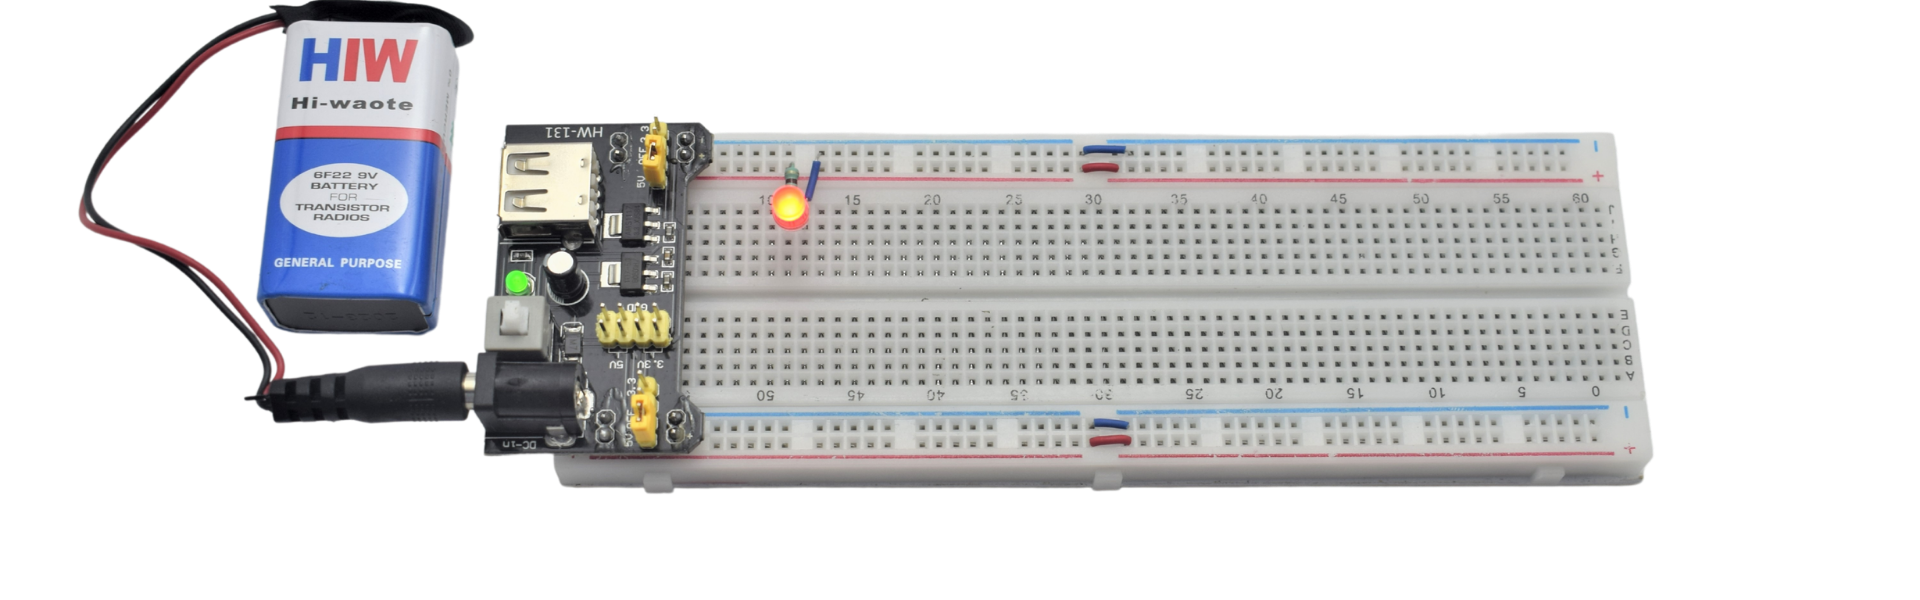
\includegraphics[width=\textwidth]{lesson_circuits/L1/L1-A.png}
    \caption{Simple Circuit on Breadboard}
    \label{fig:sc_obb}
\end{figure}



\section{Lesson 2: Lighting up an LED by pressing a Switch}
\subsection{Objective}
In this activity we'll turn on the led using a push button.
\subsection{Components Required}
\begin{enumerate}
    \item Breadboard Power Supply $\times$ 1
    \item 9V Battery $\times$ 1 
    \item 9V Battery Connector $\times$ 1
    \item Breadboard $\times$ 1
    \item 5mm Red LED $\times$ 1
    \item 220$\Omega$ resistor $\times$ 1
    \item Male to Male Jumper Wires $\times$ 2
    \item Push Button $\times$ 1
\end{enumerate}
\subsection{Circuit}
\begin{figure}[htp]
    \centering
    \begin{circuitikz}[scale = 2]
        \draw
            (0,1) to[empty led, color=red] (0,0)
            (0,0) node[ground] {}
            (0,1) to[R, l^=$R_s (220\Omega)$] (0,2)
            (0,3) to[push button] (0,2)
            (-0.2,3) -- node[anchor=south] {5V} (0.2,3);
    \end{circuitikz}
    \caption{Push Button Circuit}
    \label{fig:pb_led_circuit}
\end{figure}
\subsection{Circuit Explanation}
This circuit is similar to the one we made previously, except for the fact that we have a push button in series. The button is normally open, meaning no current flows through the circuit (no complete loop or path) and when we press the button the path is complete and LED will turn on.
\subsection{Circuit Photo}
\begin{figure}[htp]
    \centering
    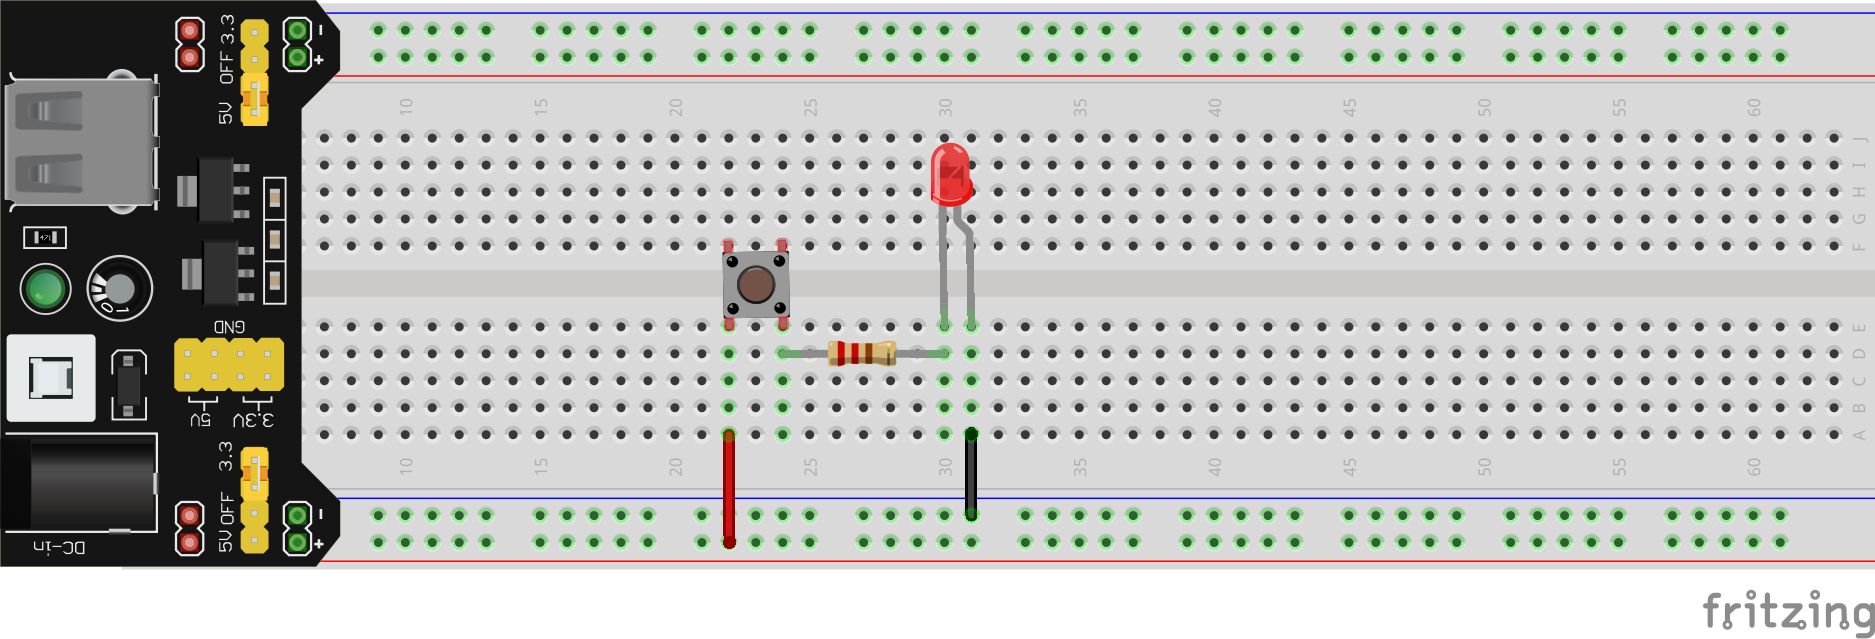
\includegraphics[width=0.8\textwidth]{lesson_circuits/L2/lesson_2.png}
    \caption{Circuit Schematic}
    \label{fig:pb_led_sch}
\end{figure}
\begin{figure}[htp]
    \centering
    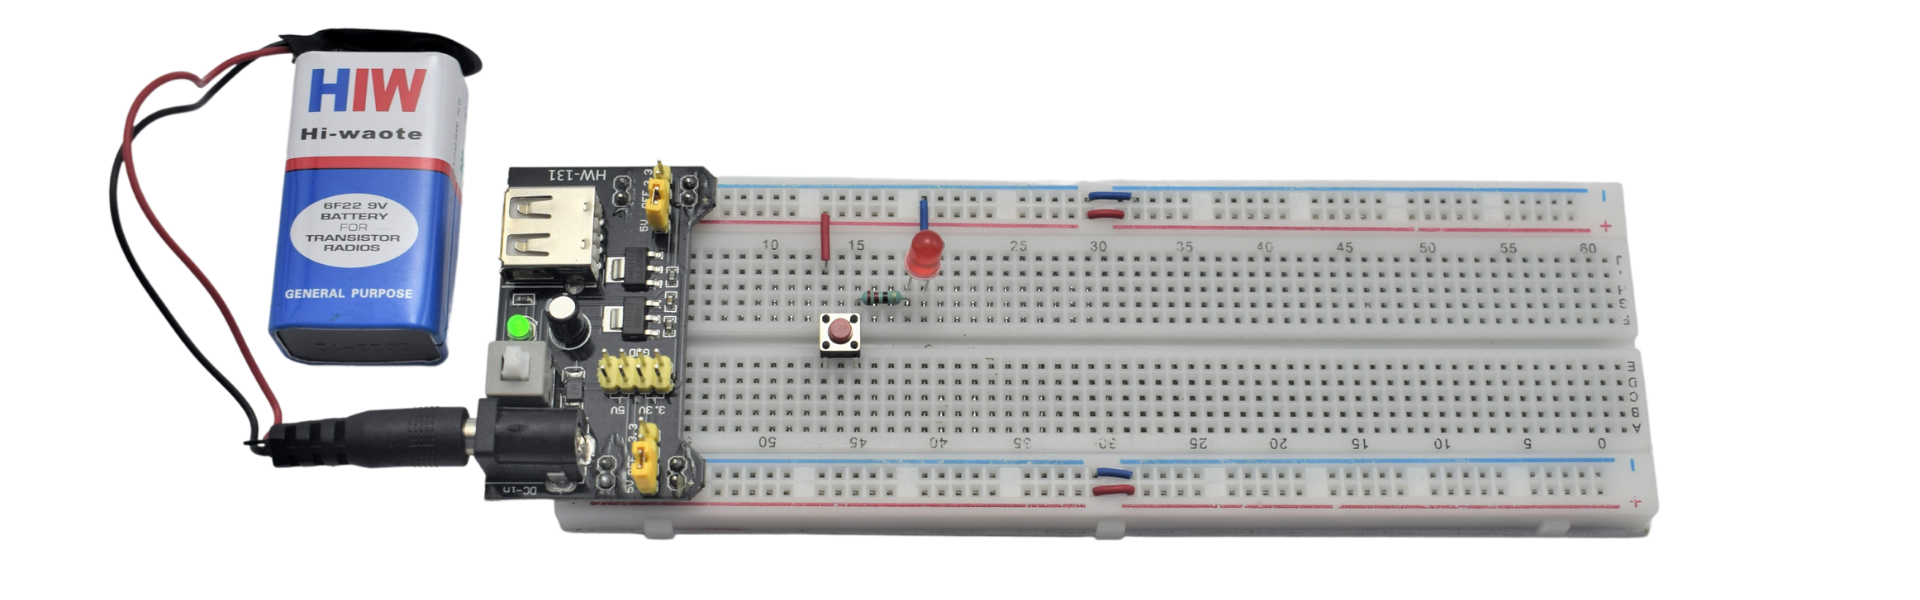
\includegraphics[width=\textwidth]{lesson_circuits/L2/L2-A.png}
    \caption{LED Off, Switch Open}
    \label{fig:pb_led_offl}
\end{figure}
\begin{figure}[htp]
    \centering
    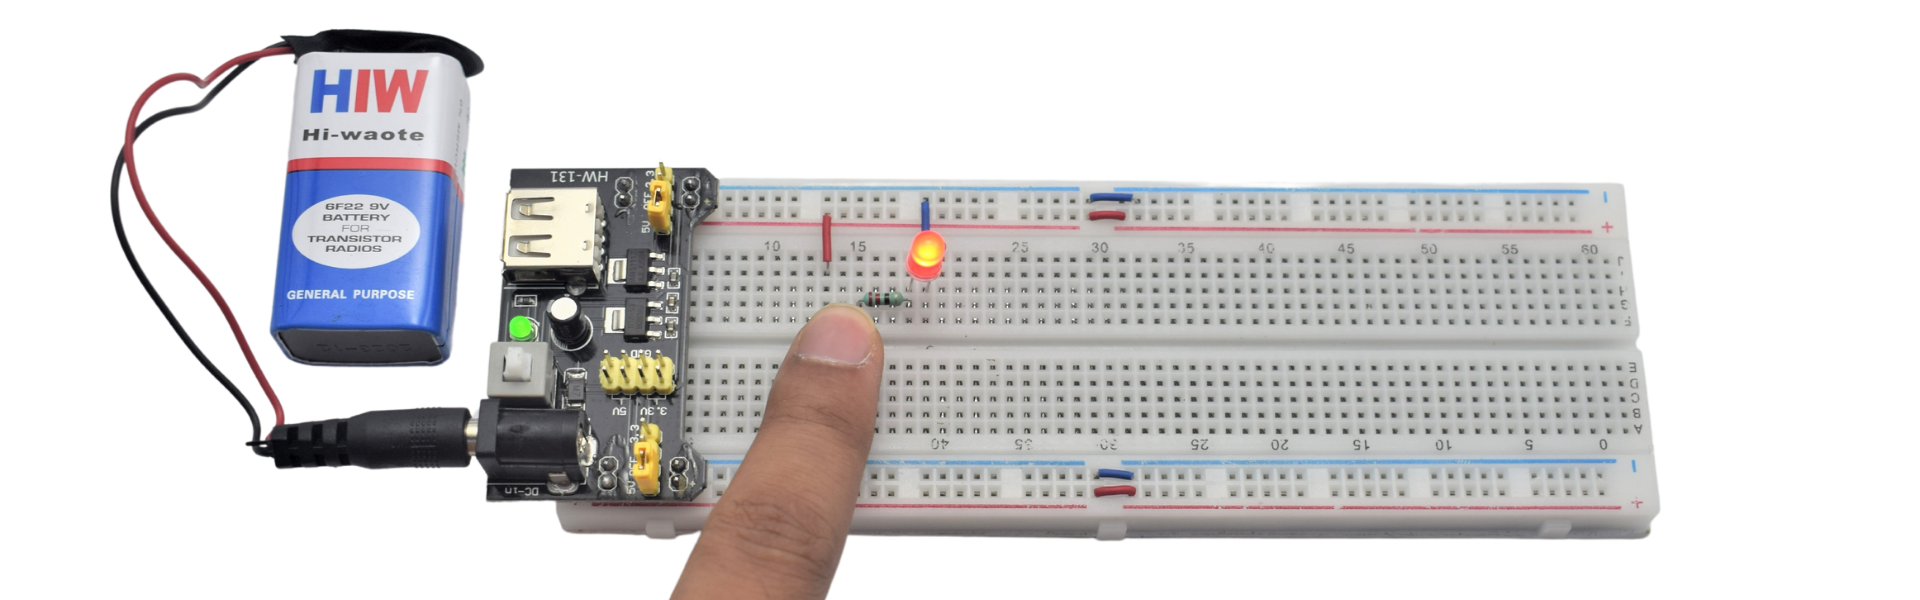
\includegraphics[width=\textwidth]{lesson_circuits/L2/L2-B.png}
    \caption{LED On, Switch Closed/Pressed}
    \label{fig:pb_led_onl}
\end{figure}



\section{Controlling LED brightness using a Potentiometer}
\subsection{Objective}
In this activity, we'll control the LED brightness/intensity with help on a potentiometer.
\subsection{Components Required}
\begin{enumerate}
    \item Breadboard Power Supply $\times$ 1
    \item 9V Battery $\times$ 1 
    \item 9V Battery Connector $\times$ 1
    \item Breadboard $\times$ 1
    \item 5mm Red LED $\times$ 1
    \item 220$\Omega$ resistor $\times$ 1
    \item Male to Male Jumper Wires $\times$ 2
    \item Potentiometer $\times$ 1
\end{enumerate}
\subsection{Circuit}
\begin{figure}[htp]
    \centering
    \begin{circuitikz}[scale = 2]
        \draw
            (0,1) to[empty led, color=red] (0,0)
            (0,0) node[ground] {}
            (0,1) to[R, l^=$R_s (220\Omega)$] (0,2)
            (0,3) to[american potentiometer, l_=$R_{pot}(\SI{10}{\kohm})$] (0,2)
            (0,2) to[short, *-] (0.5, 2) -- (0.5, 2.5) to[short, ->] (0.2, 2.5)
            (-0.2,3) -- node[anchor=south] {5V} (0.2,3);
    \end{circuitikz}
    \caption{Potentiometer LED Circuit}
    \label{fig:pot_led_circuit}
\end{figure}
\subsection{Circuit Explanation}
When the potentiometer resistance $R_{pot}$ is $0\Omega$, the LED will be in series with $R_S$ and glow. As we'll increase the resistance of potentiometer the effective series resistance will increase $R_t = R_S + R_{pot}$. With increase in the series resistance, the current through the circuit will decrease according to the Ohm's law ($I \propto \frac{1}{R}$) changing the intensity of the LED.
\subsection{Circuit Picture}
\begin{figure}[htp]
    \centering
    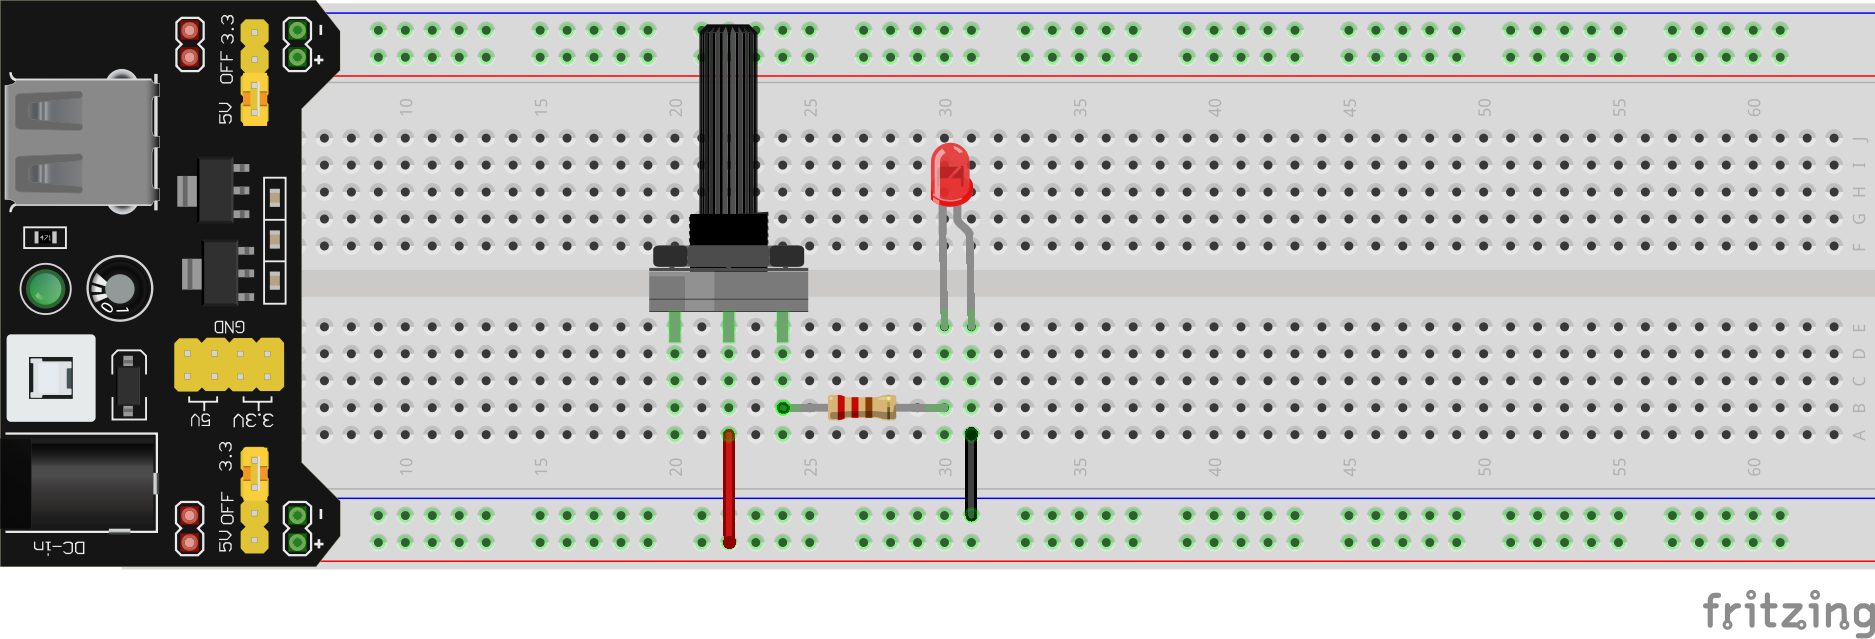
\includegraphics[width=0.8\textwidth]{lesson_circuits/L3/lesson_3.png}
    \caption{Circuit Schematic}
    \label{fig:pot_led_sch}
\end{figure}
\begin{figure}[htp]
    \centering
    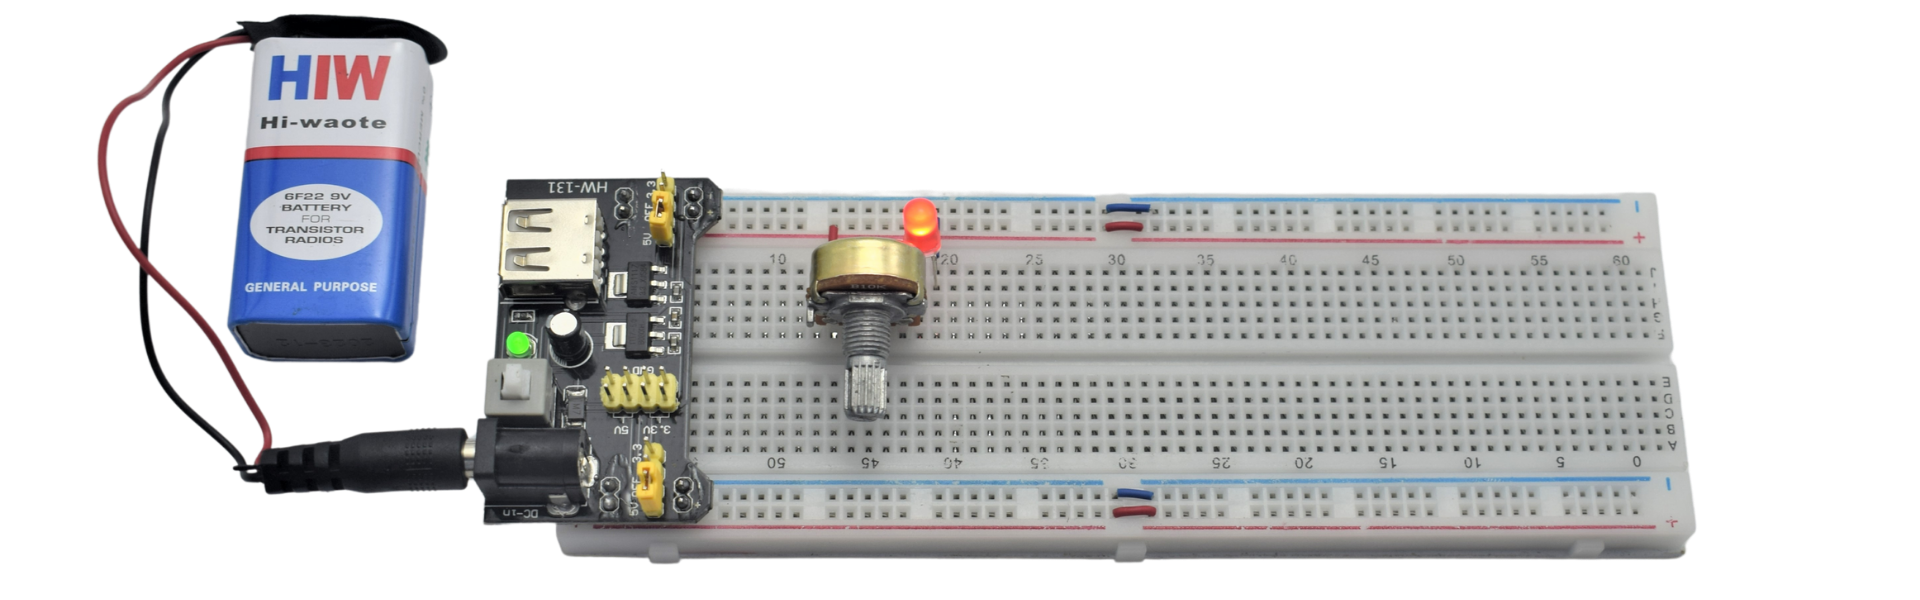
\includegraphics[width=\textwidth]{lesson_circuits/L3/L3-A.png}
    \caption{Max Intensity, $R_{pot} = 0$}
    \label{fig:pot_led_max}
\end{figure}
\begin{figure}[htp]
    \centering
    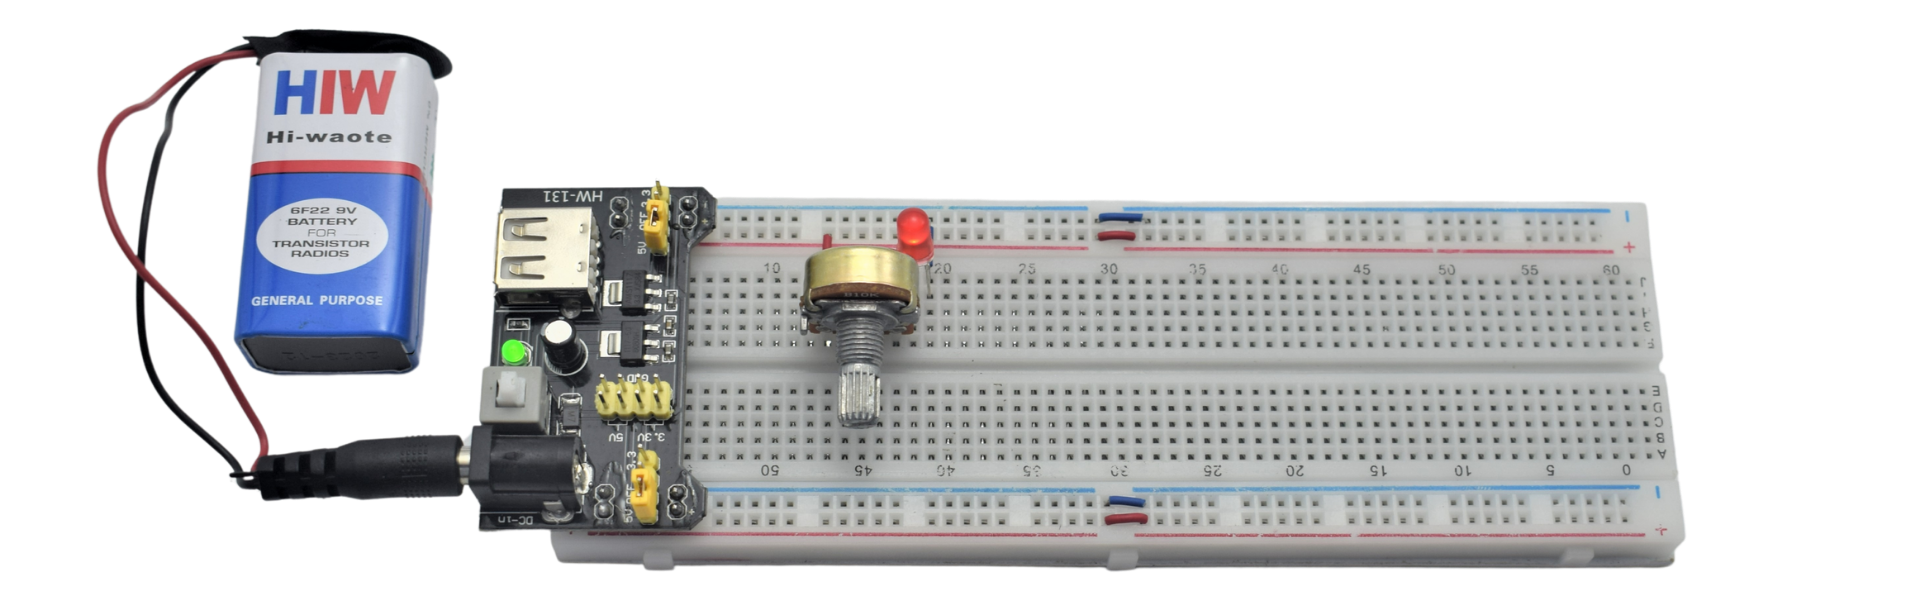
\includegraphics[width=\textwidth]{lesson_circuits/L3/L3-B.png}
    \caption{Min Intensity, $R_{pot} = 10\si{\kilo\ohm}$}
    \label{fig:pot_led_min}
\end{figure}



\section{DIY: Activities}
\begin{itemize}
    \item Calculate series resistance for RED led using 3.3V power supply
\end{itemize}
%\begin{figure}[h]
%    \centering
%    \includegraphics[width=0.77\textwidth]{ha-gray-conv-crp.jpg}
%    \caption{Picture of the M83 galaxy, image taken from the WFC3 ERS M83 Data Products, http://archive.stsci.edu/prepds/wfc3ers/m83datalist.html}
%    \label{fig:awesome_image}
%\end{figure}
%----------------------------------------------------------------------------------------
%	CHAPTER 3
%----------------------------------------------------------------------------------------

%\chapterimage{boat.png}
\cleardoublepage
\chapterimage{chap_head.png}
\chapter{Transistors}

\section{Overview}\index{Overview}
In this section you'll learn about Light Emitting Diodes (LED) and how to turn it on using different methods.

\section{Component Introduction}\index{Component Introduction!Transistors}
In this chapter we will be using transistor to make electronic circuits. There are different types of transistors available but we will be using bipolar junction transistor (BJTs) only. BJTs are the most common transistor type used among the hobbyists and DIYers.

\subsection{BJT}
A transistor is a semiconductor device with 3 terminals or regions. The interface between each of the regions forms a p-n junction, it likes two diodes together. There are two types of BJTs -
NPN, when a p-type semiconductor is in-between two n-type.
PNP, when a n-type semiconductor is in-between two p-type.
Transistors are used to amplify or switch electronic signals and electrical power. Each of the terminals or regions are named - 
\begin{itemize}
    \item Collector: The largest semiconductor region of the transistor.
    \item Emitter: The second largest semiconductor region of the transistor.
    \item Base: Middle region of the transistor. This serves as a gatekeeper that determines the amount of current that can flow through emitter-collector regions.
\end{itemize}
\begin{figure}[!htp]
    \centering
    \begin{subfigure}[b]{0.4\textwidth}
        \centering
        \begin{circuitikz}[scale = 2]
            \draw
                (0,0) node [npn](npn1){}
                (npn1.E) node[right=1mm]{E}
                (npn1.C) node[right=1mm]{C}
                (npn1.B) node[left=1mm]{B};
        \end{circuitikz}
        \caption{NPN}
    \end{subfigure}
    \hfill
    \begin{subfigure}[b]{0.4\textwidth}
        \centering
        \begin{circuitikz}[scale = 2]
            \draw
                (0,0) node [pnp](pnp1){}
                (pnp1.E) node[right=1mm]{E}
                (pnp1.C) node[right=1mm]{C}
                (pnp1.B) node[left=1mm]{B};
        \end{circuitikz}
        \caption{PNP}
    \end{subfigure}
    \caption{Transistor Symbol}
    \label{fig:bjt_symbol}
\end{figure}

\subsubsection{Operation Modes for Transistor}
There are 4 modes in which a transistor works -
\begin{enumerate}
    \item \textbf{Cut-off}
    In cut-off mode no current flows through the transistor. The transistor acts like an open circuit.
    \item \textbf{Saturation}
    In saturation mode the transistor allows current to flow freely and acts like an short-circuit.
    \item \textbf{Active}
    In active mode the amount of current flowing through the collector-emitter region is proportional to the current flowing through base.
    \item \textbf{Reverse-Active}
    It is similar to active mode, but the direction of current is reversed. The transistors are not meant to operate in Reverse-Active mode.
\end{enumerate}
If we make sure that the transistor operates in only cut-off or saturation region, then it can act like a switch turning current flow ON or OFF by controlling the base voltage. In this guide most of the circuits will use transistor in Saturation \& cut-off mode.

In NPN transistor, the base voltage should be higher than the emitter voltage by threshold voltage $V_{th}$, defined in the data-sheet of the transistor. Generally it is near about \SI{0.7}{\volt}.

For PNP, the base voltage should be lower than the emitter voltage by $V_{th}$.
\begin{figure}[!htp]
    \centering
    \begin{subfigure}[b]{0.4\textwidth}
        \centering
        \begin{circuitikz}[scale = 2]
            \draw
                (0,0) node [npn](npn1){}
                (npn1.E) node[right=1mm](n1){E}
                (npn1.C) node[right=1mm](n2){C}
                (npn1.B) node[left=1mm](n3){B};
            \draw[-latex]
                (-1,0) -- (n3);
            \draw[-latex]
                (n2) -- (n1);
        \end{circuitikz}
        \caption{NPN}
    \end{subfigure}
    \hfill
    \begin{subfigure}[b]{0.4\textwidth}
        \centering
        \begin{circuitikz}[scale = 2]
            \draw
                (0,0) node [pnp](pnp1){}
                (pnp1.E) node[right=1mm](n1){E}
                (pnp1.C) node[right=1mm](n2){C}
                (pnp1.B) node[left=1mm](n3){B};
            \draw[-latex]
                (n3) -- (-1,0);
            \draw[-latex]
                (n1) -- (n2);
        \end{circuitikz}
        \caption{PNP}
    \end{subfigure}
    \caption{Direction of Conventional current in BJTs}
    \label{fig:bjt_current}
\end{figure}

For both the transistors, $I_E = I_C + I_B$

\subsection{Capacitor}
Capacitor is a pretty simple electronic device. It consists of two conductive plates separated by an insulated medium called dielectric. Capacitors when powered are able to store energy in the form of electric field between the two plates. With different types of dielectric, there are different types of capacitors and have different qualities and uses. Capacitors can be polarized when dielectric used is polarized and favours electric field in one direction. 
\begin{figure}[!htp]
    \centering
    \begin{subfigure}[b]{0.4\textwidth}
        \centering
        \begin{circuitikz}[scale = 2]
            \draw
                (0,0) to[capacitor] (0,1);
        \end{circuitikz}
        \caption{Non Polarized}
    \end{subfigure}
    \hfill
    \begin{subfigure}[b]{0.4\textwidth}
        \centering
        \begin{circuitikz}[scale = 2]
            \draw
                (0,0) to[curved capacitor] (0,1);
        \end{circuitikz}
        \caption{Polarized}
    \end{subfigure}
    \caption{Capacitor Symbol}
    \label{fig:cap_symbol}
\end{figure}
The value of capacitor is measured in Farads (F), and one farad is a very big value. \emph{The capacitance of earth is \SI{710}{\micro\farad}}.

Capacitors or Caps are used in many ways and can be found in almost every electronic circuits.
On Polar capacitors the exact values in written on the body, for ceramic capacitor the values is written with 2 significant digits and 1 multiplier, for example capacitance of a ceramic capacitor with 105 written on it is, \num{10e4}\si{\pico\farad} = \num{e5}$\times$\num{e-12}\si{\farad} = \num{e-7}\si{\farad} = \SI{0.1}{\micro\farad}

\subsection{LDR}
Light Dependent Resistor(LDR) or photocell or photo-resistor is a semiconductor device which exhibits a very special property, it acts like a resistor but the value of resistance depends on the amount of light falling on it.

In bright light, the LDR resistance will be in the range of 0.01-10\si{\kilo\ohm} and in darkness it's resistance will be in the range of 100-1000\si{\kilo\ohm}.
\begin{figure}[!htp]
    \centering
    \begin{circuitikz}[scale = 2]
        \draw (0,0) to[sR] (1,0);
    \end{circuitikz}
    \caption{LDR Symbol}
    \label{fig:ldr_symbol}
\end{figure}

\subsection{RGB LED}
RGB LED is a combination of all three LEDs (RED, GREEN, BLUE) in one single package. You can produce different colors using RGB LEDs by configuring the intensity of each LED.

There are two kinds of RGB LED, one shares the cathode pin and the other shares the anode pin.
\begin{figure}[!htp]
    \centering
    \begin{subfigure}[b]{0.4\textwidth}
        \centering
        \begin{circuitikz}[scale = 2]
        \draw (0,0) to[short, *-] (0,0) -- ++(0,-0.5);
        \draw (0,0) to[full led, invert, color=green] (0,1);
        \draw (0,0) -- (0.5,0) to[full led, invert, color=red] (0.5,1);
        \draw (0,0) -- (-0.5,0) to[full led, invert, color=blue] (-0.5,1);
        \end{circuitikz}
        \caption{Common Anode}
    \end{subfigure}
    \hfill
    \begin{subfigure}[b]{0.4\textwidth}
        \centering
        \begin{circuitikz}[scale = 2]
        \draw (0,0) to[short, *-] (0,0) -- ++(0,-0.5);
        \draw (0,0) to[full led, color=green] (0,1);
        \draw (0,0) -- (0.5,0) to[full led, color=red] (0.5,1);
        \draw (0,0) -- (-0.5,0) to[full led, color=blue] (-0.5,1);
        \end{circuitikz}
        \caption{Common Cathode}
    \end{subfigure}
    \caption{RGB LED Symbol}
    \label{fig:rgb_symbol}
\end{figure}

\clearpage

\section{Lesson 4: Astable Multivibrator}
\subsection{Objective}
In this activity, we will make an astable multivibrator using BJTs and flash two LEDs.
\subsection{Components Required}
\begin{enumerate}
    \item Breadboard Power Supply $\times$ 1
    \item 9V Battery $\times$ 1
    \item 9V Battery Connector $\times$ 1
    \item Breadboard $\times$ 1
    \item Red LED $\times$ 2
    \item \SI{220}{\ohm} $\times$ 2
    \item \SI{100}{\kilo\ohm} $\times$ 2
    \item 2N2222 NPN Transistor $\times$ 2
    \item \SI{10}{\micro\farad} $\times$ 2
    \item Male-Male jumper wire $\times$ 6
\end{enumerate}
\subsection{Circuit}
\begin{figure}[!htp]
    \centering
    \begin{circuitikz}[scale = 2]
        \draw (0,0) node[ground]{};
        \draw (-1,0.5) node[npn](npn1){T1};
        \draw (1,0.5) node[npn, xscale=-1](npn2){\scalebox{-1}[1]{T2}};
        \draw (npn1.E) -- (-1,0) -- (0,0);
        \draw (npn2.E) -- (1,0) to[short, -*] (0,0);
        \draw (npn1.B) -- (-2,0.5) -- (-2,2) to[R, l^=$R_1$] (-2,3);
        \draw (npn2.B) -- (2,0.5) -- (2,2) to[R, l_=$R_4$] (2,3);
        \draw (-2,3) to[short, -*] (-1,3) 
            to[R, l^=$R_2$] (-1,2)
            to[empty led, mirror, l_=$L1$] (npn1.C);
        \draw (2,3) to[short, -*] (1,3) 
            to[R, l_=$R_3$] (1,2)
            to[empty led, l=$L2$] (npn2.C);
        \draw (-1,3) to[short, -*] (0,3) -- (1,3);
        \draw (npn1.C) to[short, *-] ++(0.7,0) to[C,l=$C_{2}$]
            ++(0, 1) to[short, -*] (2,1.9);
        \draw (npn2.C) to[short, *-] ++(-0.7,0) to[C,l_=$C_{1}$]
            ++(0, 1.1) to[short, -*] (-2,2);
        \draw (0,3) node[vcc](vcc1){$V_{CC}$};
    \end{circuitikz}
    \caption{Astable Multivibrator}
    \label{fig:astable_multivibrator}
\end{figure}
\subsection{Circuit Explanation}
Let's assume that $T1$ has just turned off and $T2$ has just turned on which means $C_2$ is fully charged and $C_1$ is discharged. Since, $T1$ is in cut-off mode, the collector $T1.C$ will rise to $V_{cc}$ potential and the potential across the $C_2$ capacitor will  be $V_{cc} - V_{th}$, where $V_{th}$ is the threshold voltage of transistors. 

$T2$ is fully on, the capacitor $C_1$ will start charging through resistor $R_1$ and the $LED_1$ will be turned on. When the plate of $C_1$ connected to base of $T1$ rises to potential $V_{th}$ it will pull $T1$ into conduction and then saturation mode. When the transistor $T1$ is in saturation mode it will immediately pull the capacitor $C_1$ to ground, this rapid change in voltage at the plate of capacitor $C_1$ connected to $T1.C$ causes an equal and instantaneous fall in voltage at the plate connected to base of $T2$, turning it hard off. Now $T1$ is On turning $LED_1$ on and $T2$ is off and the same cycle repeats again, $C2$ starts charging turning $T2$ on and $C1$ turning $T1$ off.
\begin{figure}[!htp]
    \centering
    \begin{circuitikz}[scale = 2]
        \draw (0,0) node[ground]{};
        \draw (-1,0.5) node[npn](npn1){T1};
        \draw (1,0.5) node[npn, xscale=-1](npn2){\scalebox{-1}[1]{T2}};
        \draw (npn1.E) -- (-1,0) -- (0,0);
        \draw (npn2.E) -- (1,0) to[short, -*] (0,0);
        \draw (npn1.B) -- (-2,0.5) -- (-2,2) to[R, l^=$R_1$] (-2,3);
        \draw (npn2.B) -- (2,0.5) -- (2,2) to[R, l_=$R_4$] (2,3);
        \draw (-2,3) to[short, -*] (-1,3) 
            to[R, l^=$R_2$] (-1,2)
            to[empty led, mirror, l_=$L1$] (npn1.C);
        \draw (2,3) to[short, -*] (1,3) 
            to[R, l_=$R_3$] (1,2)
            to[empty led, l=$L2$] (npn2.C);
        \draw (-1,3) to[short, -*] (0,3) -- (1,3);
        \draw (npn1.C) to[short, *-] ++(0.7,0) to[C,l=$C_{2}$]
            ++(0, 1) to[short, -*] (2,1.9);
        \draw (npn2.C) to[short, *-] ++(-0.7,0) to[C,l_=$C_{1}$]
            ++(0, 1.1) to[short, -*] (-2,2);
        \draw (0,3) node[vcc](vcc1){$V_{CC}$};
        \draw[-latex, red]
            (-2.4,3) -- (-2.4,2.1) 
            -- (0.1,2.1) -- (0.1,0.75) 
            -- (0.9,0.75) -- (0.9,0.1);
        \draw (npn1.C) node[right=10mm](n1c){};
        \draw (npn1.E) node[right=10mm](n1b){};
        \draw[-latex, blue] (n1b) -- (n1c);
        \draw (npn1.C) node[left=0.2mm](){$T1.C$};
    \end{circuitikz}
    \caption{T1 off, T2 on}
    \label{fig:astable_working}
\end{figure}

The time period or frequency of oscillation for astable multivibrator can be calculated using the below equations - 
\begin{align*}
    t_1 &= 0.693 \times R_1 \times C_1 \\
    t_2 &= 0.693 \times R_4 \times C_2
\end{align*}
where, $t_1$ \& $t_2$ are charging and discharging time period for the capacitors.

For symmetrical astable multivibrator $R_1 = R_2$ and $C_1 = C_2$.

The total time period is -
\begin{align*}
    T &= t_1 + t_2 \\
    T &= 0.693RC + 0.693RC \\
    T &= 1.386RC
\end{align*}
In our circuit we will use $R_2 = R_3 = 220\si{\ohm}$, $R_1 = R_4 = 100\si{\kilo\ohm}$ and $C_1 = C_2 = 10\si{\micro\farad}$.

By changing the values of series RC we have change the time period of oscillation.
\subsection{Circuit Picture}
\begin{figure}[!htp]
    \centering
    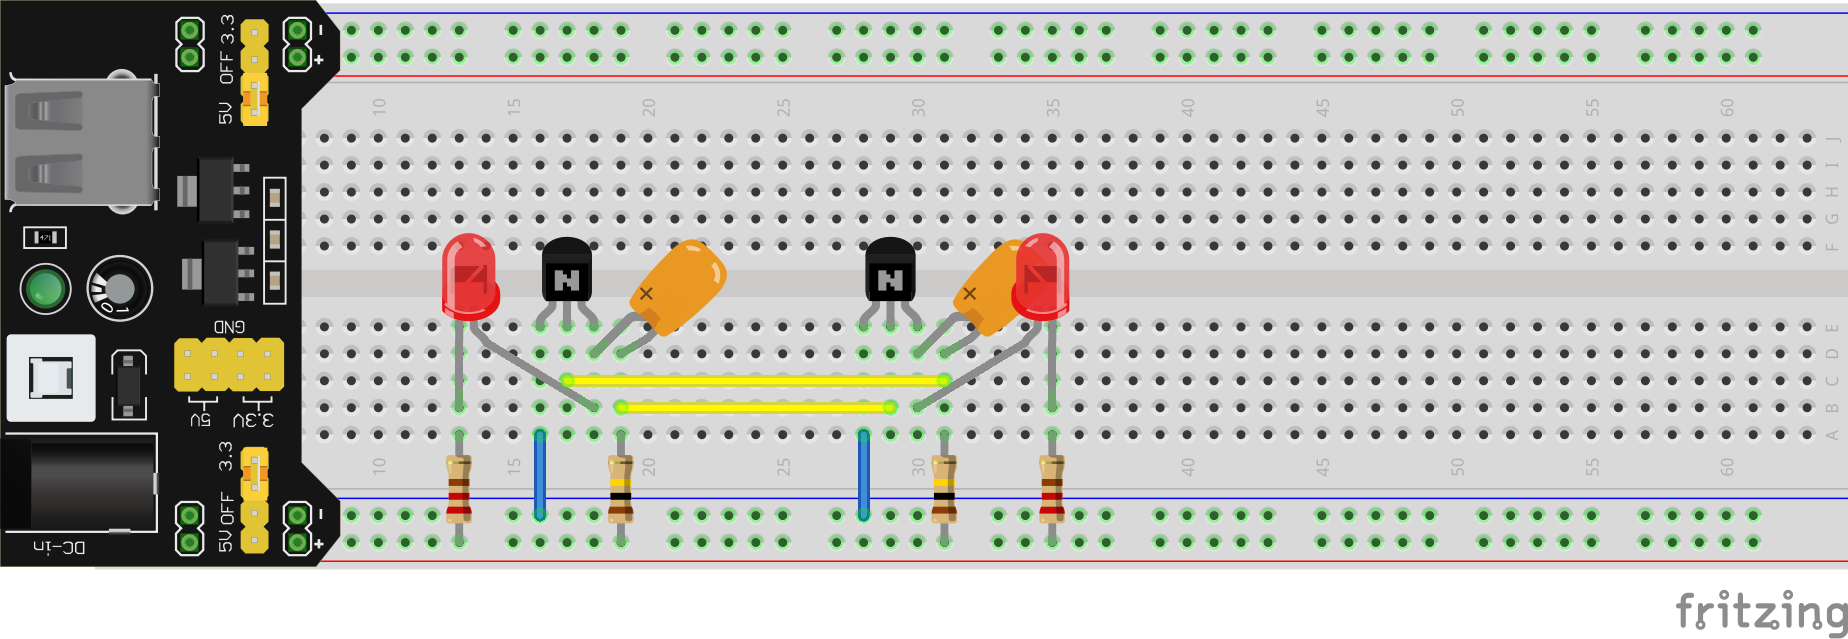
\includegraphics[width=0.8\textwidth]{lesson_circuits/L4/lesson_4.png}
    \caption{Circuit Schematic}
    \label{fig:asm_sch}
\end{figure}
\begin{figure}[!htp]
    \centering
    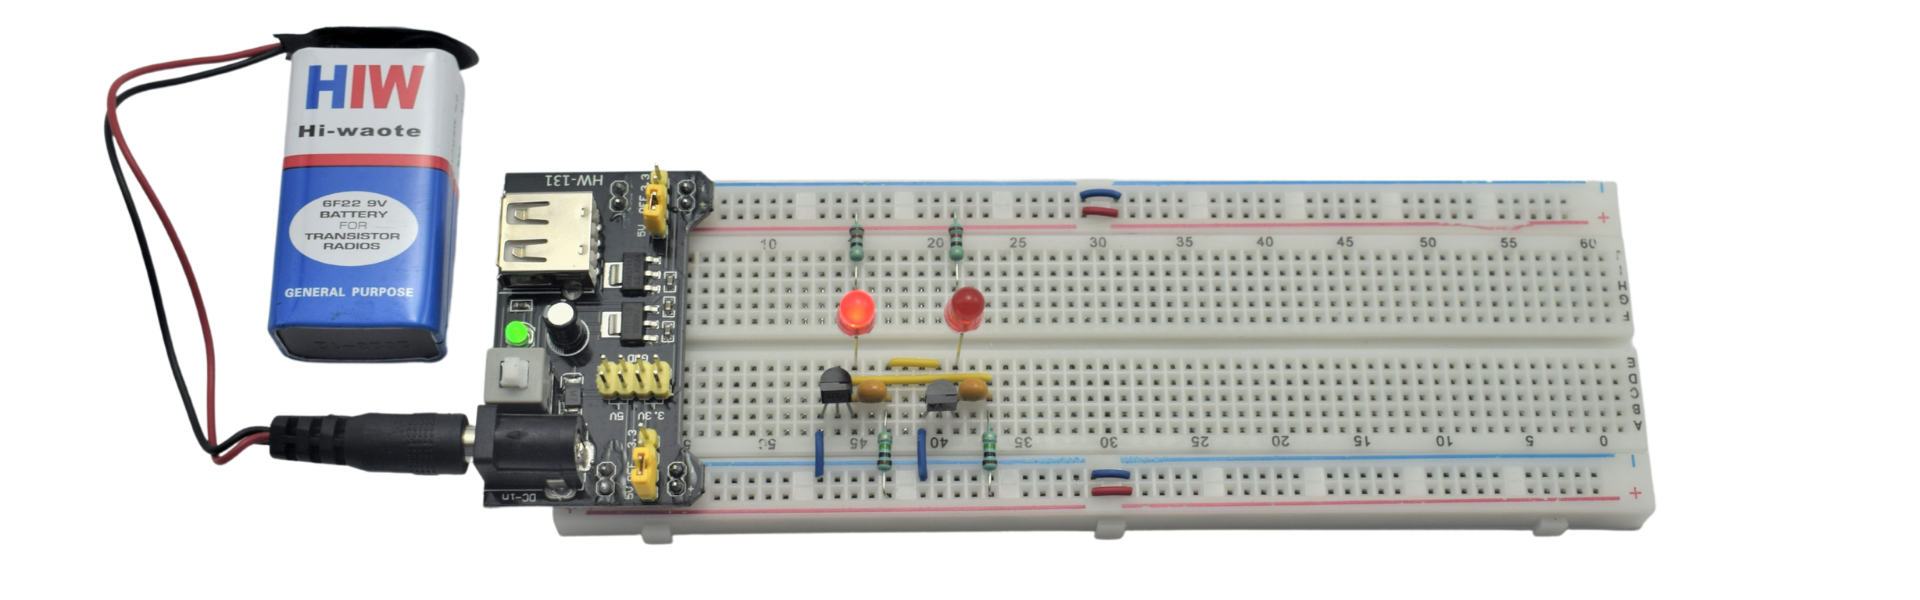
\includegraphics[width=\textwidth]{lesson_circuits/L4/L4-A.png}
    \caption{Astable Multivibrator Breadboard Schematic}
    \label{fig:asm_obb}
\end{figure}



\section{Lesson 5: Transistor as Touch Sensor}
\subsection{Objective}
In this activity we will build a very basic touch sensor using transistors.
\subsection{Components Required}
\begin{enumerate}
    \item Breadboard Power Supply $\times$ 1
    \item 9V Battery $\times$ 1
    \item 9V Battery Connector $\times$ 1
    \item Breadboard $\times$ 1
    \item Red LED $\times$ 1
    \item \SI{220}{\ohm} $\times$ 1
    \item \SI{10}{\kilo\ohm} $\times$ 1
    \item 2N2222 NPN Transistor $\times$ 2
    \item Male pin header $\times$ 2
    \item Male-Male jumper wire $\times$ 5
\end{enumerate}
\subsection{Circuit}
\begin{figure}[!htp]
    \centering
    \begin{circuitikz}[scale = 2]
        \draw (0,0) node[npn](npn1){$T2=2N2222$};
        \draw (npn1.E) node[ground]{};
        \draw (-2,1.5) node[npn](npn2){$T1=2N2222$};
        \draw (npn1.B) to[R, l^=$\SI{10}{\kilo\ohm}$] ++(-1,0) -| (npn2.E);
        \draw ($(npn1.C)+(0,3)$) node[vcc](vcc1){VCC=\SI{5}{\volt}} to[R, l=$\SI{220}{\ohm}$] ($(npn1.C)+(0,2)$)
        to[empty led] (npn1.C);
        \draw (npn2.C) -| ++(0,1.5) to[short, -*] (vcc1);
        \draw (npn2.B) to[short, -o] ++(-0.57,0);
        \draw (npn2.C) to[short, *-o] ++(-1,0);
        \node[left=40,above=4] at (npn2.B) {Touch};
    \end{circuitikz}
    \caption{Transistors as Touch Sensor}
    \label{fig:transistor_touch_circuit}
\end{figure}
\subsection{Circuit Explanation}
By default both the transistors are turned off. When you touch the male pin headers connected between $VCC$ and the base of $T1$, you body acts like a resistor between them, allowing a very small current($I_{B1}$) to pass through the base of $T1$. This current is not sufficient to push $T1$ into saturation.

Therefore, we have connected the base of $T2$ to the emitter of $T1$ and the base current($I_{B2}$) for $T2$ is approximately equal to the collector current($I_{C1}$) of $T1$, which is $\beta \times I_{B1}$. This current is sufficient to pull the $T2$ transistor into saturation mode and the LED turn on.
\begin{figure}[!htp]
    \centering
    \begin{circuitikz}[scale = 2]
        \draw (0,0) node[npn](npn1){$2N2222$};
        \draw (npn1.E) node[ground](gnd1){};
        \draw (-2,1.5) node[npn](npn2){$2N2222$};
        \draw (npn1.B) to[R, l^=$\SI{10}{\kilo\ohm}$] ++(-1,0) -| (npn2.E);
        \draw ($(npn1.C)+(0,3)$) node[vcc](vcc1){VCC=\SI{5}{\volt}} to[R, l=$\SI{220}{\ohm}$] ($(npn1.C)+(0,2)$)
        to[empty led] (npn1.C);
        \draw (npn2.C) -| ++(0,1.5) to[short, -*] (vcc1);
        \draw (npn2.B) to[short, -o] ++(-0.57,0);
        \draw (npn2.C) to[short, *-o] ++(-1,0);
        \draw[red] ($(npn2.C)+(-1,0)$) -- ++(0,0.5)
                to[short, -o] ++(-1,0) 
                node[](T1){};
        \draw[red] ($(npn2.B)+(-0.57,0)$) -- ++(0,-0.5)
                to[short, -o] ++(-1,0)
                node[](T2){};
        \draw[red] (T1) to[R, l_=$R_{Body}$] (T2);
        \node[left=40,above=4] at (npn2.B) {Touch};
        \draw[-latex, orange]
            ($(T2)+(0,-0.2)$) -- ++(1.2,0)
            -- ++(0,0.5) -- ++(0.5,0) node[midway,below]{$I_{B1}$};
        \draw[-latex, green]
            ($(npn2.E)-(0.2,0.2)$) |- ($(npn1.B)+(0,0.2)$)
            node[midway,above left, text width=6mm]{$I_{B2}$ $I_{C1}$};
        \draw[-latex, red]
            ($(vcc1)+(0.3,0)$) -- ($(gnd1)+(0.3,0)$)
            node[midway,right]{$I_{C2}$};
    \end{circuitikz}
    \caption{Touch Sensor Working}
    \label{fig:transistor_touch_working}
\end{figure}
\subsection{Circuit Picture}
\begin{figure}[!htp]
    \centering
    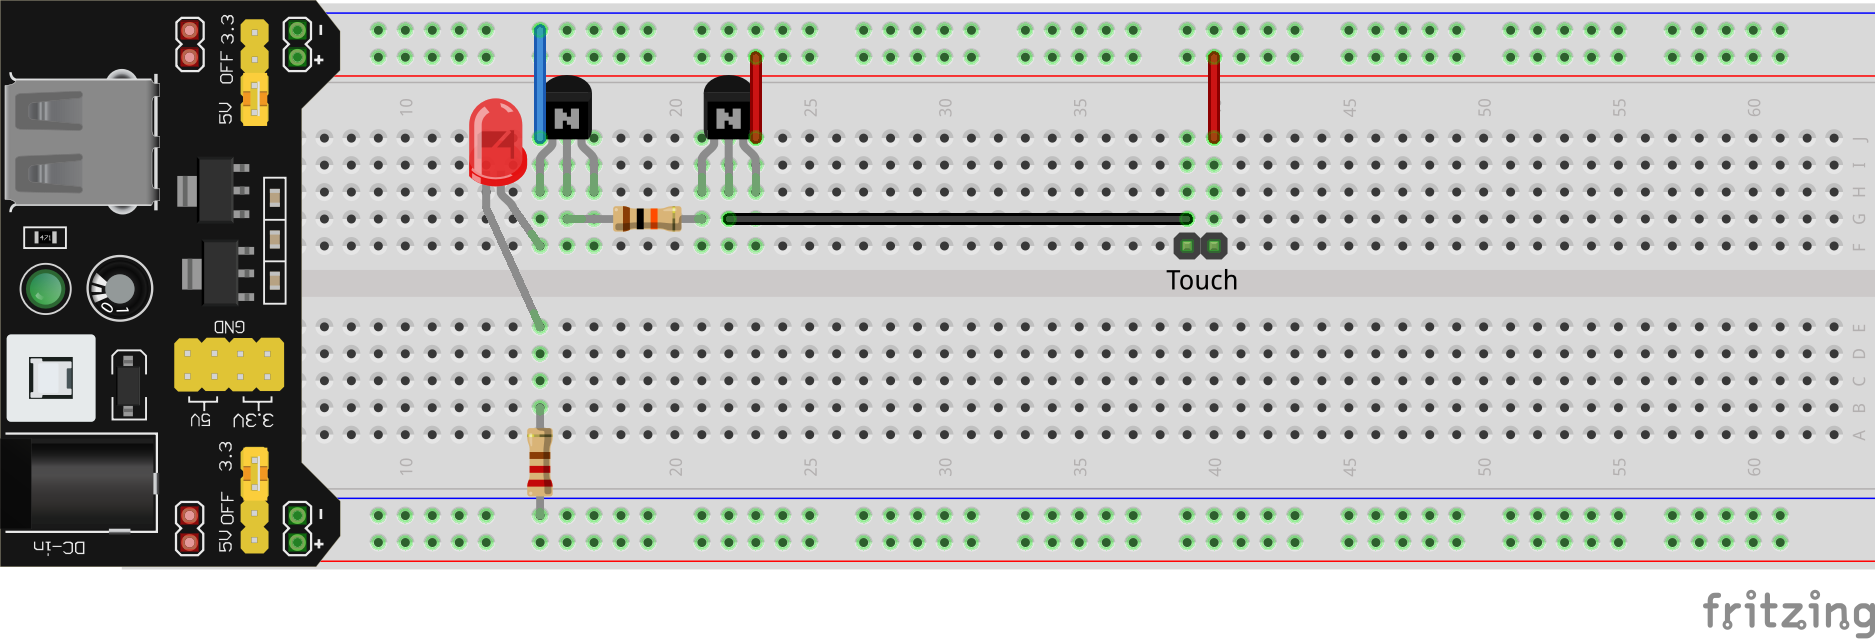
\includegraphics[width=0.8\textwidth]{lesson_circuits/L5/lesson_5.png}
    \caption{Breadboard Schematic}
    \label{fig:simple_touch_sch}
\end{figure}
\begin{figure}[!htp]
    \centering
    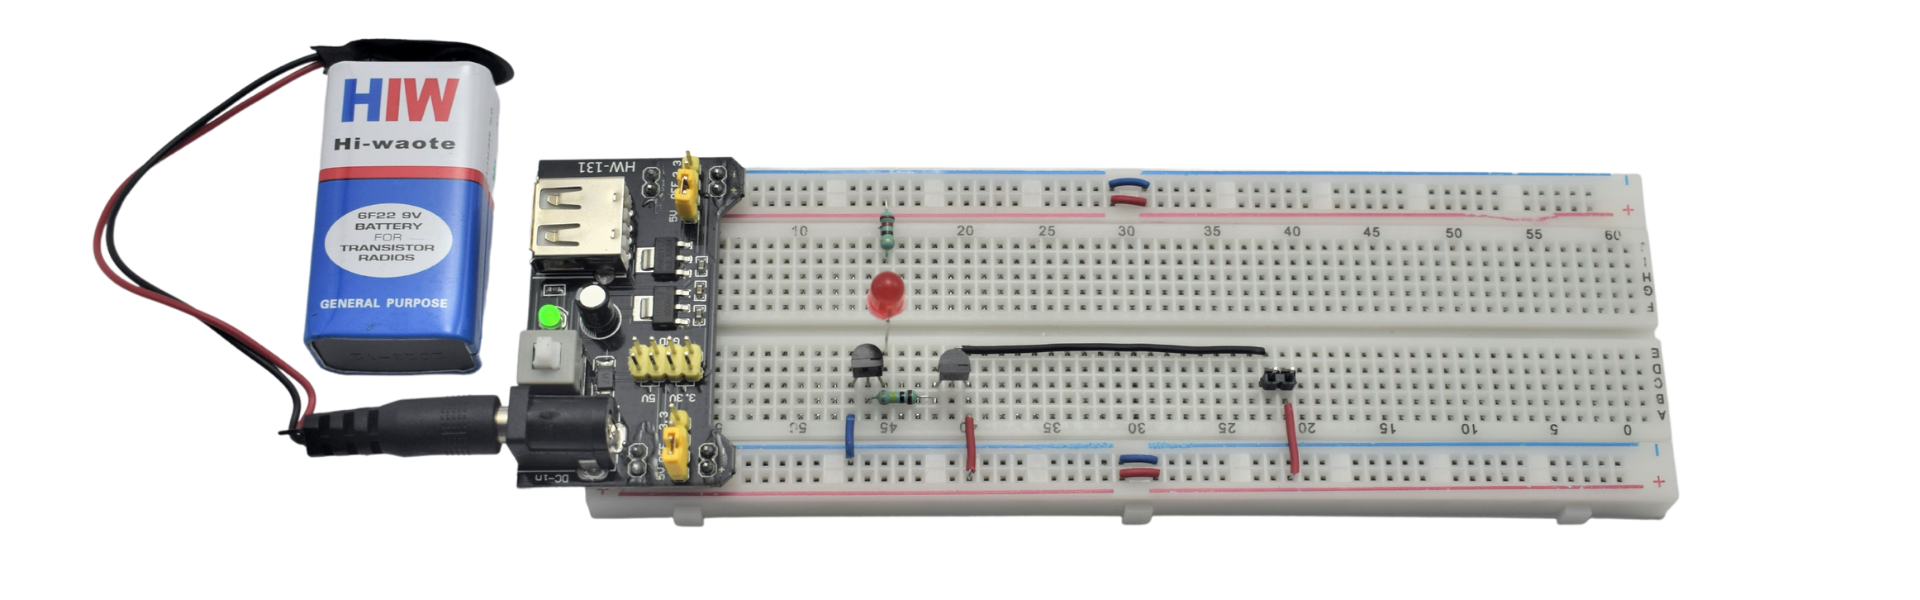
\includegraphics[width=\textwidth]{lesson_circuits/L5/L5-A.png}
    \caption{Touch Switch on Breadboard}
    \label{fig:stouch_obb}
\end{figure}
\begin{figure}[!htp]
    \centering
    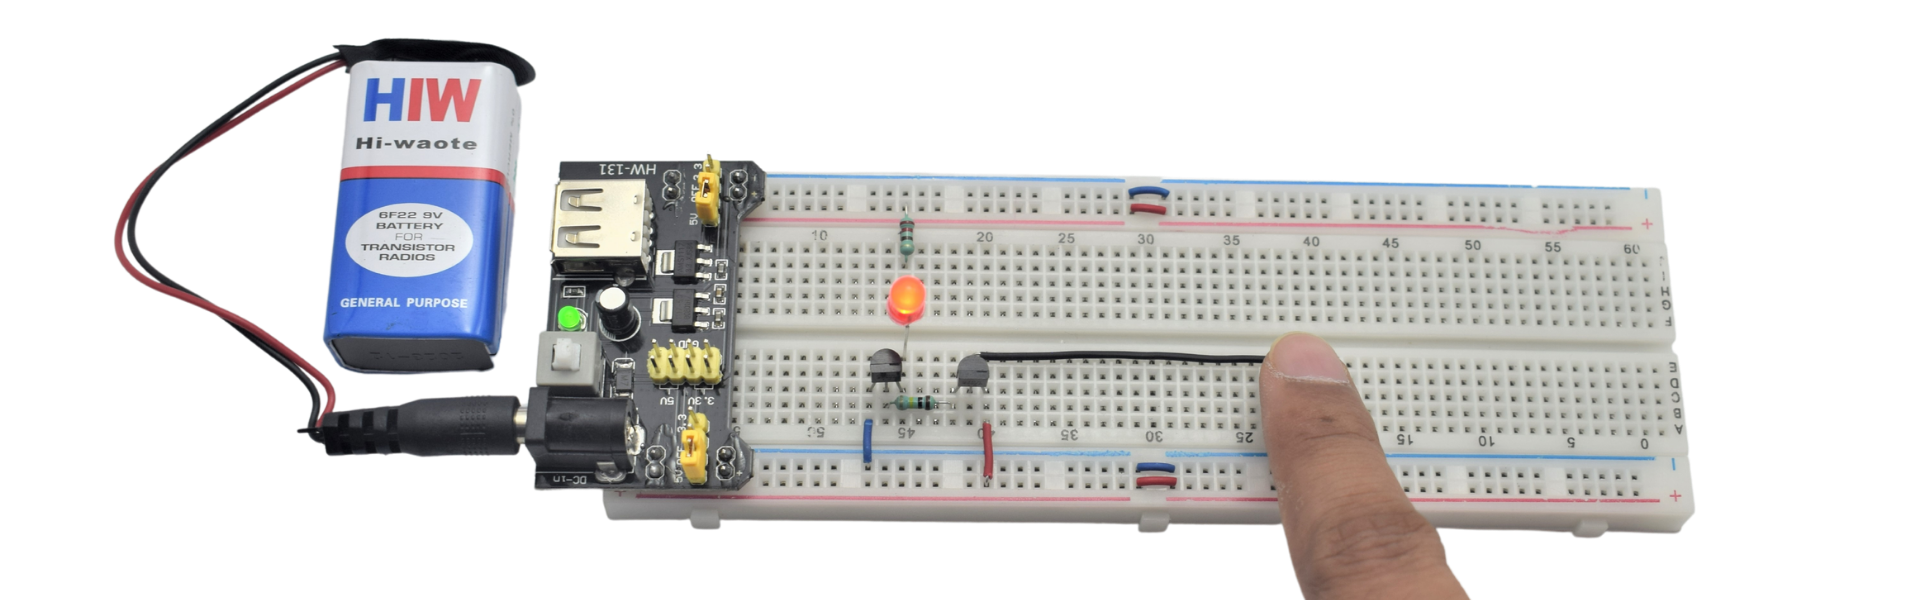
\includegraphics[width=\textwidth]{lesson_circuits/L5/L5-B.png}
    \caption{Touch Switch on Breadboard - LED glows on touching the pin headers}
    \label{fig:stouch_on_obb} 
\end{figure}


\section{Lesson 6: Flip Flop}
\subsection{Objective}
In this activity we'll use transistors and push buttons to make a flip flop circuit.
\subsection{Components Required}
\begin{enumerate}
    \item Breadboard Power Supply $\times$ 1
    \item 9V Battery $\times$ 1
    \item 9V Battery Connector $\times$ 1
    \item Breadboard $\times$ 1
    \item Red LED $\times$ 2
    \item \SI{1}{\kilo\ohm} $\times$ 2
    \item \SI{100}{\kilo\ohm} $\times$ 2
    \item 2N2222 NPN Transistor $\times$ 2
    \item 10-XX Push Buttons $\times$ 2
    \item Male-Male jumper wire $\times$ 8
\end{enumerate}
\subsection{Circuit}
\begin{figure}[!htp]
    \centering
    \begin{circuitikz}[scale = 2]
        \draw (2, 0) node[npn](npn1){$T_1=2N2222$};
        \draw ( -2, 0) node[npn, xscale=-1](npn2){\scalebox{-1}[1]{$T_2=2N2222$}};
        \draw (npn2.E) to[short, -*] ++(1.5,0)
                to[short, -*] ++(0.5,0)
                node[ground]{}
                to[short, -*] ++(0.5,0)
                to[short] (npn1.E);
        \draw (npn1.C) -- ++(0,1)
                to[empty led, invert, mirror, l=$L_1$] ++(0,1)
                to[R, l=$\SI{1}{\kilo\ohm}$] ++(0,1) -- ++(-2,0);
        \draw (npn2.C) -- ++(0,1)
                to[empty led, invert, l_=$L_2$] ++(0,1)
                to[R, l=$\SI{1}{\kilo\ohm}$] ++(0,1)
                to[short, -*] ++(2,0)
                node[vcc]{VCC};
        \draw[orange] ($(npn2.E)+(1.5,0)$) to[push button, l=$B_2$] ++(0,1)
                    |- ++(1,0.5)
                    to[R, l=$\SI{100}{\kilo\ohm}$] ++(1,0) 
                    to[short,-*] ++(0.5,0);
        \draw[red] ($(npn1.E)-(1.5,0)$) to[push button, mirror, l_=$B_1$] ++(0,1)
                    |- ++(-1,0.7)
                    to[R, l_=$\SI{100}{\kilo\ohm}$] ++(-1,0) 
                    to[short,-*] ++(-0.5,0);
        \draw[orange] (npn2.B) -| ++(0.5,0.7)
                    to[short, -*] ++(0.575,0);
        \draw[red] (npn1.B) -| ++(-0.5,0.7)
            to[short, -*] ++(-0.575,0);
    \end{circuitikz}
    \caption{Flip Flop}
    \label{fig:flip_flop}
\end{figure}
\subsection{Circuit Explanation}
Let's assume that $L_1$ is on, which means there is a very small amount of current flowing through the $L_2$ to the base of transistor $T_1$. The current flowing through $L_1$ will prefer to go through the transistor $T_1$ because this path offers the least resistance.

Now, when we press the button $B_1$ the current going to the base of $T_1$ will now directly go to the ground, switching $T_1$ off. And there will be a small current going through the led $L_1$ to the base of transistor $T_2$, pushing it into saturation. And when we leave the button $B_1$ the current through $L_2$ will go through $T_2$ only, as it will offer a path with least resistance.
\begin{figure}[!htp]
    \centering
    \begin{circuitikz}[scale = 2]
        \draw (2, 0) node[npn](npn1){$T_1=2N2222$};
        \draw ( -2, 0) node[npn, xscale=-1](npn2){\scalebox{-1}[1]{$T_2=2N2222$}};
        \draw (npn2.E) to[short, -*] ++(1.5,0)
                to[short, -*] ++(0.5,0)
                node[ground]{}
                to[short, -*] ++(0.5,0)
                to[short] (npn1.E);
        \draw (npn1.C) -- ++(0,1)
                to[empty led, invert, mirror, l=$L_1$] ++(0,1)
                to[R, l=$\SI{1}{\kilo\ohm}$] ++(0,1) -- ++(-2,0);
        \draw (npn2.C) -- ++(0,1)
                to[empty led, invert, color=red, l_=$L_2$] ++(0,1)
                to[R, l_=$\SI{1}{\kilo\ohm}$] ++(0,1)
                to[short, -*] ++(2,0)
                node[vcc]{VCC};
        \draw[orange] ($(npn2.E)+(1.5,0)$) to[push button, l=$B_2$] ++(0,1)
                    |- ++(1,0.5)
                    to[R, l=$\SI{100}{\kilo\ohm}$] ++(1,0) 
                    to[short,-*] ++(0.5,0);
        \draw[red] ($(npn1.E)-(1.5,0)$) to[normally closed push button, mirror, l_=$B_1$] ++(0,1)
                    |- ++(-1,0.7)
                    to[R, l_=$\SI{100}{\kilo\ohm}$] ++(-1,0) 
                    to[short,-*] ++(-0.5,0);
        \draw[orange] (npn2.B) -| ++(0.5,0.7)
                    to[short, -*] ++(0.575,0);
        \draw[red] (npn1.B) -| ++(-0.5,0.7)
            to[short, -*] ++(-0.575,0);
        \draw[-latex, color=brown] 
            (2.4, 3.2) -- (2.4, 0.9) -- (-1.3,0.9) -- (-1.3,0.2) -- (-1.5,0.2);
        \draw[-latex, color=red] 
            (-2.4, 3.2) to[short,-*] (-2.4, 1.15) -- (0.3,1.15) -- (0.3,0);
        \draw[-latex, color=red] 
            (-2.4, 3.2) -- (-2.4, 0);
    \end{circuitikz}
    \caption{Flip Flop Working}
    \label{fig:flip_flop_working}
\end{figure}
\subsection{Circuit Picture}
\begin{figure}[!htp]
    \centering
    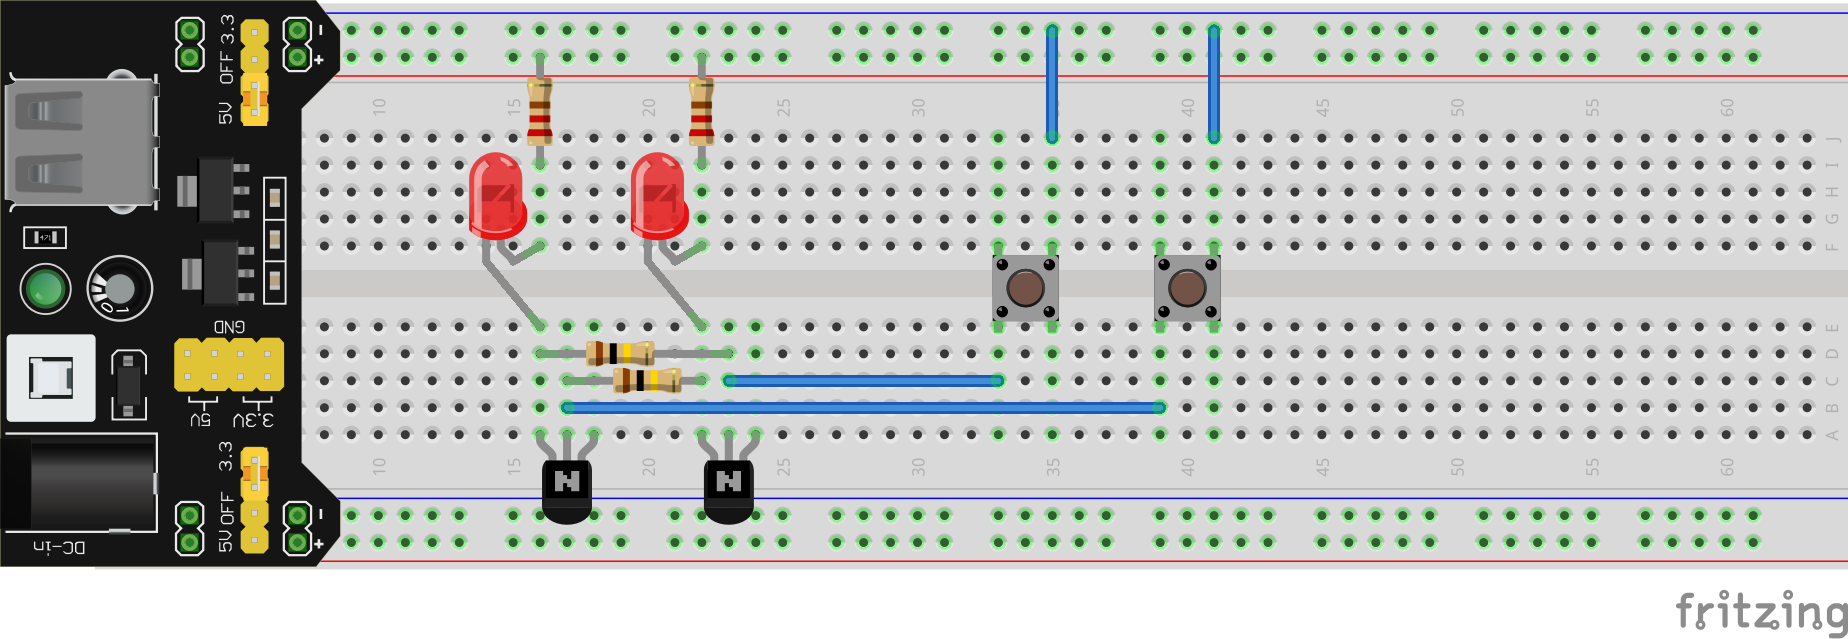
\includegraphics[width=0.8\textwidth]{lesson_circuits/L6/lesson_6.png}
    \caption{Breadboard Schematic}
    \label{fig:ff_bjt_sch}
\end{figure}
\begin{figure}[!htp]
    \centering
    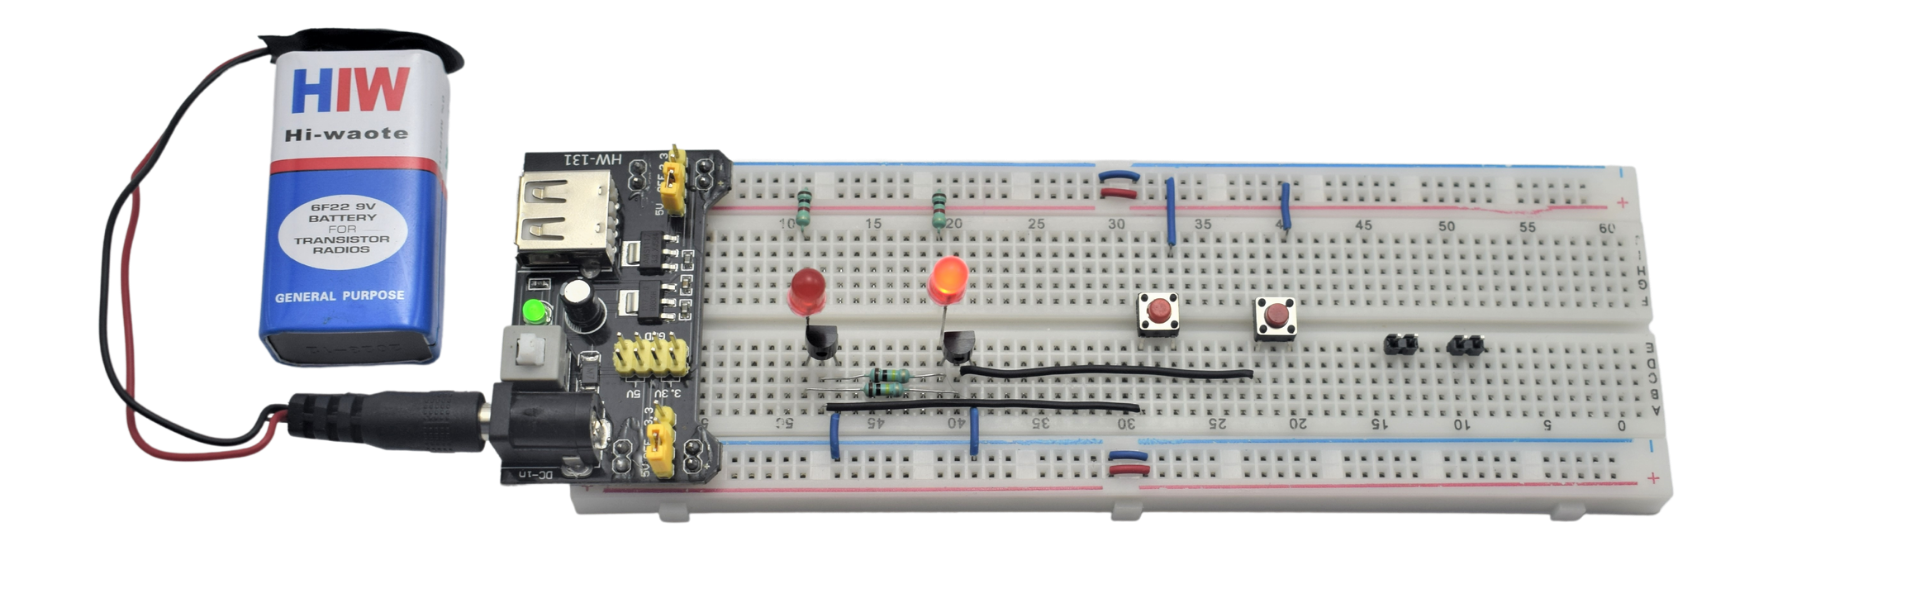
\includegraphics[width=\textwidth]{lesson_circuits/L6/L6-A.png}
    \caption{Flip/Flop using BJTs on Breadboard}
    \label{fig:ff_obb1}
\end{figure}
\begin{figure}[!htp]
    \centering
    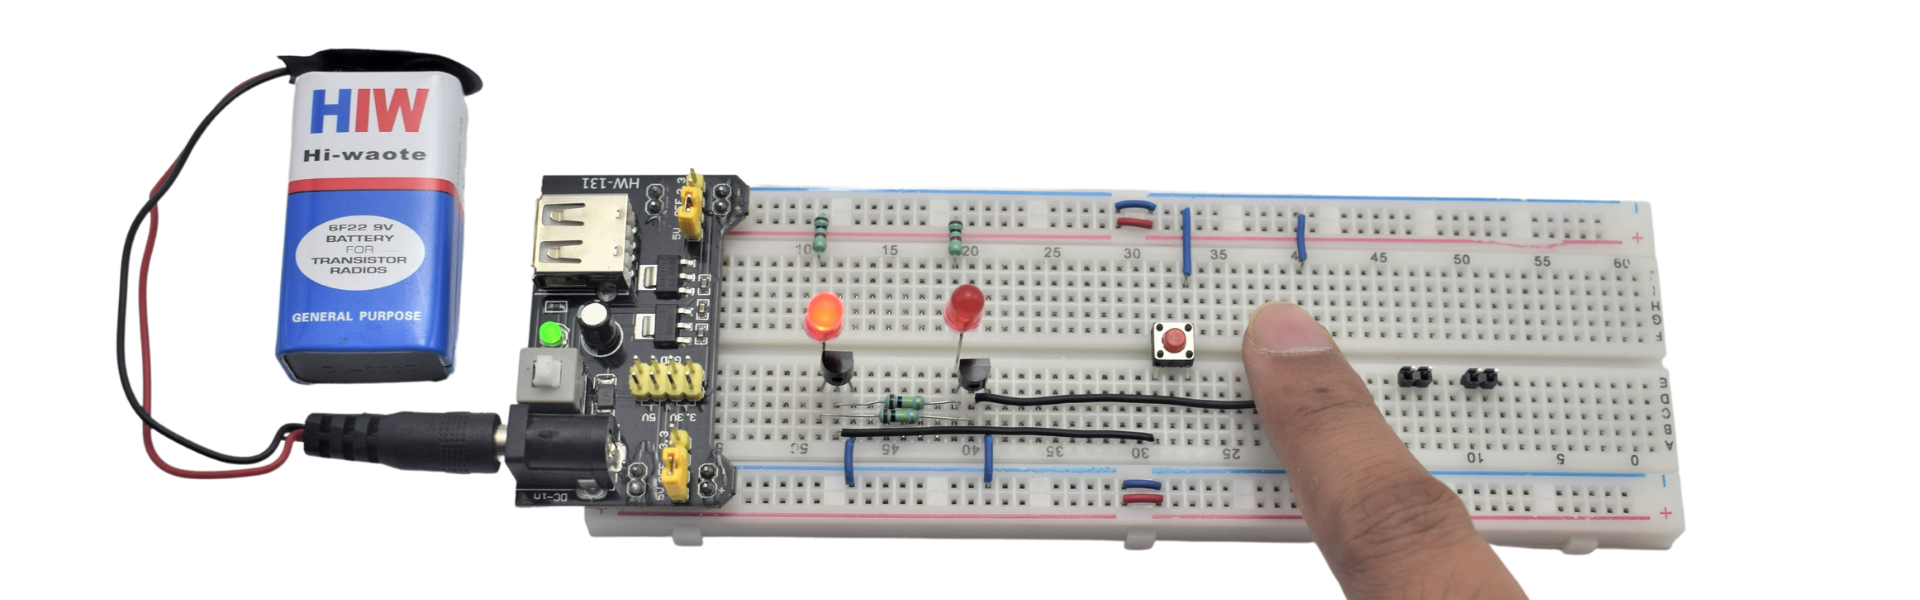
\includegraphics[width=\textwidth]{lesson_circuits/L6/L6-B.png}
    \caption{Flip/Flop using BJTs on Breadboard}
    \label{fig:ff_obb2}
\end{figure}
\begin{figure}[!htp]
    \centering
    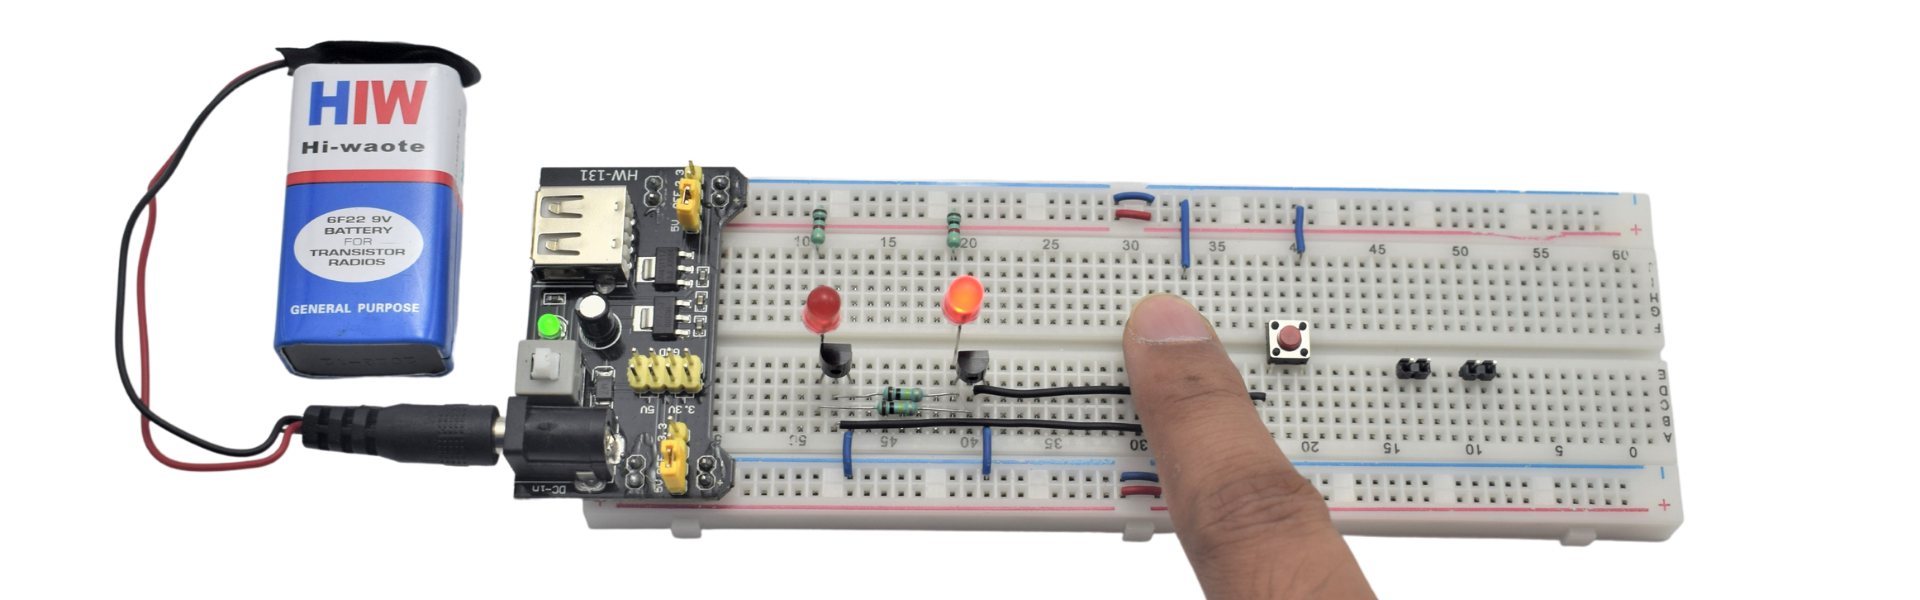
\includegraphics[width=\textwidth]{lesson_circuits/L6/L6-C.png}
    \caption{Flip/Flop using BJTs on Breadboard}
    \label{fig:ff_obb3}
\end{figure}
\begin{figure}[!htp]
    \centering
    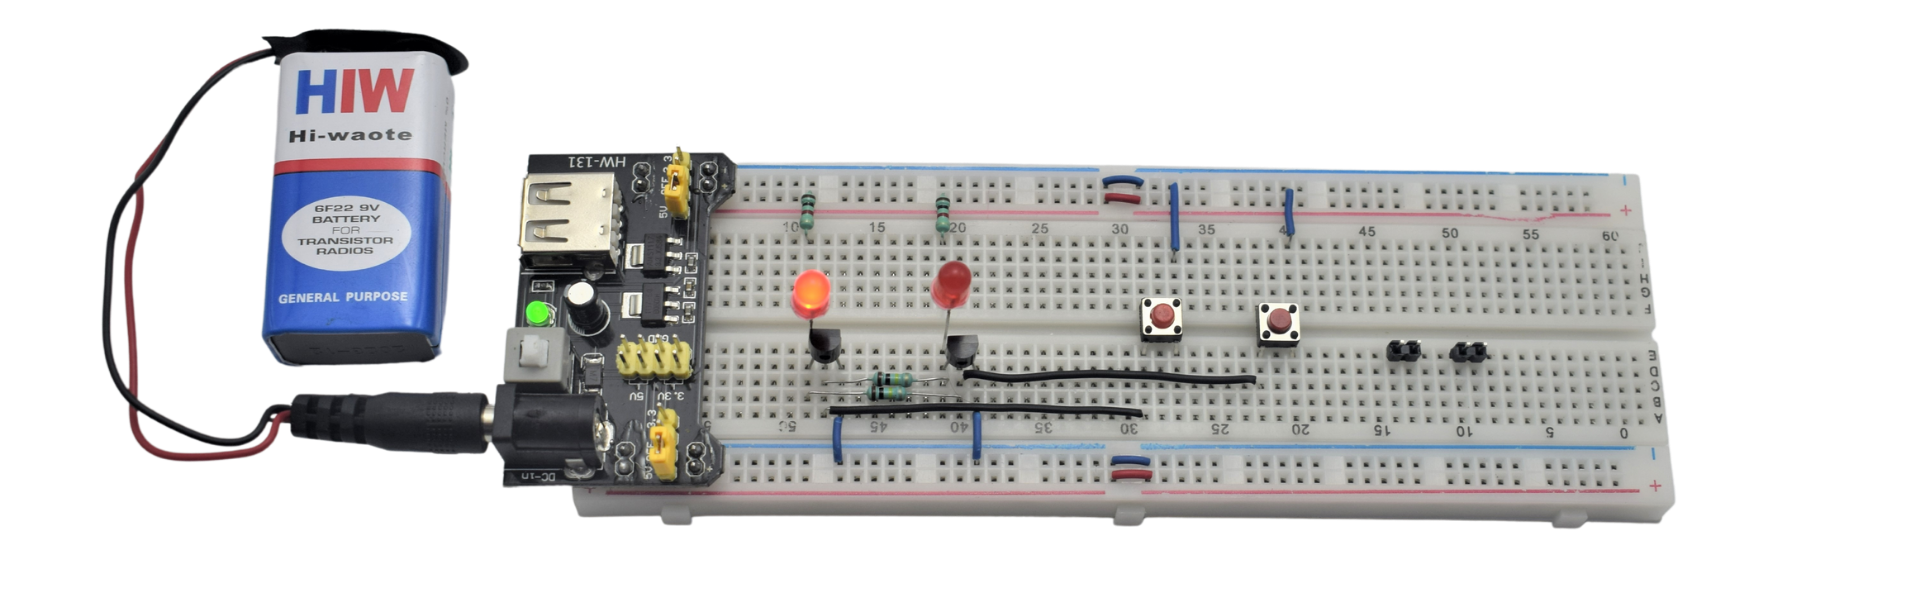
\includegraphics[width=\textwidth]{lesson_circuits/L6/L6-D.png}
    \caption{Flip/Flop using BJTs on Breadboard}
    \label{fig:ff_obb4}
\end{figure}


\section{Lesson 7: On/Off Touch using Transistors}
\subsection{Objective}
In this activity we will make an on off touch switch using transistors, which will remember its state.
\subsection{Components Required}
\begin{enumerate}
    \item Breadboard Power Supply $\times$ 1
    \item 9V Battery $\times$ 1
    \item 9V Battery Connector $\times$ 1
    \item Breadboard $\times$ 1
    \item Red LED $\times$ 1
    \item \SI{220}{\ohm} $\times$ 1
    \item \SI{10}{\kilo\ohm} $\times$ 1
    \item \SI{100}{\kilo\ohm} $\times$ 1
    \item 2N2222 NPN Transistor $\times$ 3
    \item 2N2907 PNP Transistor $\times$ 1
    \item Male pin headers $\times$ 4
    \item Male-Male jumper wire $\times$ 13
\end{enumerate}
\subsection{Circuit}
\begin{figure}[!htp]
    \centering
    \begin{circuitikz}[scale = 2]
        \draw (1.5,3) node[pnp](t1){T1};
        \draw (0,2.5) node[npn](t2){T2};
        \draw (-1,2) node[npn](t3){T3};
        \draw (-2,3.5) node[npn](t4){T4};
        \draw (t3.E) |- (0,0)
                node[ground]{} 
                to[short, *-] (t2.E);
        \draw (0,0) -- (1.5,0)
                to[empty led, invert, mirror] ++(0,0.75);
        \draw[red] (1.5,0.75) to[R, l_=$\SI{200}{\ohm}$] ++(0,0.75)
                to[short, *-] (t1.C);
        \draw[purple] (1.5,1.5) to[R, l^=$\SI{100}{\kilo\ohm}$] ++(-2,0)
                to[short, -*] ++(0,1);
        \draw[purple] (t3.C) to[short, -*] ++(0,0.11);
        \draw[purple] (t2.B) to[short, -o] ++(-4,0);
        \draw[green] (t4.E) |- (t3.B);
        \draw[green] (t4.B) to[short, -o] ++(-2,0);
        \draw[red] (t1.E) |- (0,4) node[vcc](vcc1){VCC};
        \draw[red] (vcc1) to[short, *-*] (-2,4) -- (t4.C);
        \draw[red] (-2,4) -- (-3,4)
                to[short, -*] (-3,3.7) 
                to[short, -o] ++(-1.42,0);
        \draw[red] (-3, 3.7) -- (-3,2.7)
                to[short, -o] ++(-1.42,0);
        \draw (vcc1) to[R, l=$\SI{10}{\kilo\ohm}$] (t2.C);
        \draw[blue] (t1.B) to[short, -*] (0,3);
        \draw[green] (-4.7,3.6) node[]{OFF};
        \draw[red] (-4.7,2.6) node[]{ON};
    \end{circuitikz}
    \caption{On/Off Touch Switch using Transistors}
    \label{fig:on_off_transistor}
\end{figure}
\subsection{Circuit Explanation}
When we touch the pin headers marked \emph{on}, we introduce our body resistance between $VCC$ and base of transistor $T2$, turning it on. When $T2$ is turned on, it pulls the base of transistor $T1$ to ground, pushing it to saturation mode. A small part of the current flowing through the collector of $T1$ goes to the base of $T2$ through feedback resistor. Now, when we remove our body resistance from the circuit the current through feedback keeps $T2$ on, which make sure the $T1$ is on and the led is glowing.
\begin{figure}[!htp]
    \centering
    \begin{circuitikz}[scale = 2]
        \draw (1.5,3) node[pnp](t1){T1};
        \draw (0,2.5) node[npn](t2){T2};
        \draw (-1,2) node[npn](t3){T3};
        \draw (-2,3.5) node[npn](t4){T4};
        \draw (t3.E) |- (0,0)
                node[ground]{} 
                to[short, *-] (t2.E);
        \draw (0,0) -- (1.5,0)
                to[empty led, invert, mirror] ++(0,0.75);
        \draw[red] (1.5,0.75) to[R, l_=$\SI{200}{\ohm}$] ++(0,0.75)
                to[short, *-] (t1.C);
        \draw[purple] (1.5,1.5) to[R, l^=$\SI{100}{\kilo\ohm}$] ++(-2,0)
                to[short, -*] ++(0,1);
        \draw[purple] (t3.C) to[short, -*] ++(0,0.11);
        \draw[purple] (t2.B) to[short, -o] ++(-3,0)  node[](o1){};
        \draw[green] (t4.E) |- (t3.B);
        \draw[green] (t4.B) to[short, -o] ++(-2,0);
        \draw[red] (t1.E) |- (0,4) node[vcc](vcc1){VCC};
        \draw[red] (vcc1) to[short, *-*] (-2,4) -- (t4.C);
        \draw[red] (-2,4) -- (-3,4)
                to[short, -*] (-3,3.7) 
                to[short, -o] ++(-1.42,0);
        \draw[red] (-3, 3.7) -- (-3,2.7)
                to[short, -o] ++(-0.42,0) node[](o2){};
        \draw (vcc1) to[R, l=$\SI{10}{\kilo\ohm}$] (t2.C);
        \draw[blue] (t1.B) to[short, -*] (0,3);
        \draw[green] (-4.7,3.6) node[]{OFF};
        \draw[red] (-3.7,2.6) node[]{ON};
        \draw[red]
            (o2) -- ++(0,0.5) 
            to[short, -o] ++(-1,0) node[](r1){};
        \draw[red]
            (o1) -- ++(0,-0.5) 
            to[short, -o] ++(-1,0) node[](r2){};
        \draw[red]
            (r1) to[R, l_=$R_{Body}$] (r2);
        \draw[-latex, brown]
            ($(r2)+(0,-0.2)$) -- ++(1.2,0) -- ++(0,0.5) -- ++(2.9,0) node[midway,below=3mm,left=6mm]{$I_{B2}$};
        \draw[-latex, orange]
            ($(t1.E)+(0.3,0)$) to[short,-*] ++(0,-1.6) -- ++(0,-1.3) node[midway, right=4mm, above=6mm]{$I_{led}$};
        \draw[-latex, orange]
            ($(t1.E)+(0.3,-1.6)$) -- ++(-2,0) -- ++(0,0.5) node[midway,right =8mm]{$I_{feedback}$};
    \end{circuitikz}
    \caption{Touch Switch using Transistors - On State}
    \label{fig:on_off_transistor_on_working}
\end{figure}

Now, when we touch the pin header marked \emph{off}, we introduce our body resistance in between the $VCC$ and the base of $T4$, turning it on. The $T4$ collector current goes to the base of $T3$, turning it on. There are two things that causes the led to turn off, base of $T2$ is pulled to ground, and the feedback current keeping it on goes to ground via $T3$. It means $T2$ is switched off, and when $T2$ is off the base of $T1$ is pulled high, turning it hard off.
\begin{figure}[!htp]
    \centering
    \begin{circuitikz}[scale = 2]
        \draw (1.5,3) node[pnp](t1){T1};
        \draw (0,2.5) node[npn](t2){T2};
        \draw (-1,2) node[npn](t3){T3};
        \draw (-2,3.5) node[npn](t4){T4};
        \draw (t3.E) |- (0,0)
                node[ground]{} 
                to[short, *-] (t2.E);
        \draw (0,0) -- (1.5,0)
                to[empty led, invert, mirror] ++(0,0.75);
        \draw[red] (1.5,0.75) to[R, l_=$\SI{200}{\ohm}$] ++(0,0.75)
                to[short, *-] (t1.C);
        \draw[purple] (1.5,1.5) to[R, l^=$\SI{100}{\kilo\ohm}$] ++(-2,0)
                to[short, -*] ++(0,1);
        \draw[purple] (t3.C) to[short, -*] ++(0,0.11);
        \draw[purple] (t2.B) to[short, -o] ++(-4,0);
        \draw[green] (t4.E) |- (t3.B);
        \draw[green] (t4.B) to[short, -o] ++(-1,0) node[](o1){};
        \draw[red] (t1.E) |- (0,4) node[vcc](vcc1){VCC};
        \draw[red] (vcc1) to[short, *-*] (-2,4) -- (t4.C);
        \draw[red] (-2,4) -- (-3,4)
                to[short, -*] (-3,3.7) 
                to[short, -o] ++(-0.42,0) node[](o2){};
        \draw[red] (-3, 3.7) -- (-3,2.7)
                to[short, -o] ++(-1.42,0);
        \draw (vcc1) to[R, l=$\SI{10}{\kilo\ohm}$] (t2.C);
        \draw[blue] (t1.B) to[short, -*] (0,3);
        \draw[green] (-3.7,3.6) node[]{OFF};
        \draw[red] (-4.7,2.6) node[]{ON};
        \draw[red]
            (o2) -- ++(0,0.5) 
            to[short, -o] ++(-1,0) node[](r1){};
        \draw[red]
            (o1) -- ++(0,-0.5) 
            to[short, -o] ++(-1,0) node[](r2){};
        \draw[red]
            (r1) to[R, l_=$R_{Body}$] (r2);
        \draw[-latex, brown]
            ($(r2)+(0,-0.1)$) -- ++(1.1,0) -- ++(0,0.5) -- ++(1,0) node[midway,below=3mm,right=1mm]{$I_{B4}$};
        \draw[-latex, brown]
            ($(t4.E)+(0.2,0)$) -- ++(0,-0.9) -- ++(0.5,0);
        \draw[-latex, orange]
            ($(t3.E)+(-0.2,0)$) -- ++(0,-1.5)
            node[midway, left=4mm, above=1mm]{$I_{C3}$};
        \draw[-latex, orange]
            ($(t1.E)+(0.2,-1.7)$) -- ++(-2,0) -- ++(0,0.5) node[midway,right =8mm]{$I_{feedback}$}
            -- ++(-0.5,0) -- ++(0,-2);
    \end{circuitikz}
    \caption{Touch Switch using Transistors - Off State}
    \label{fig:on_off_transistor_off_working}
\end{figure}

\subsection{Circuit Picture}
\begin{figure}[!htp]
    \centering
    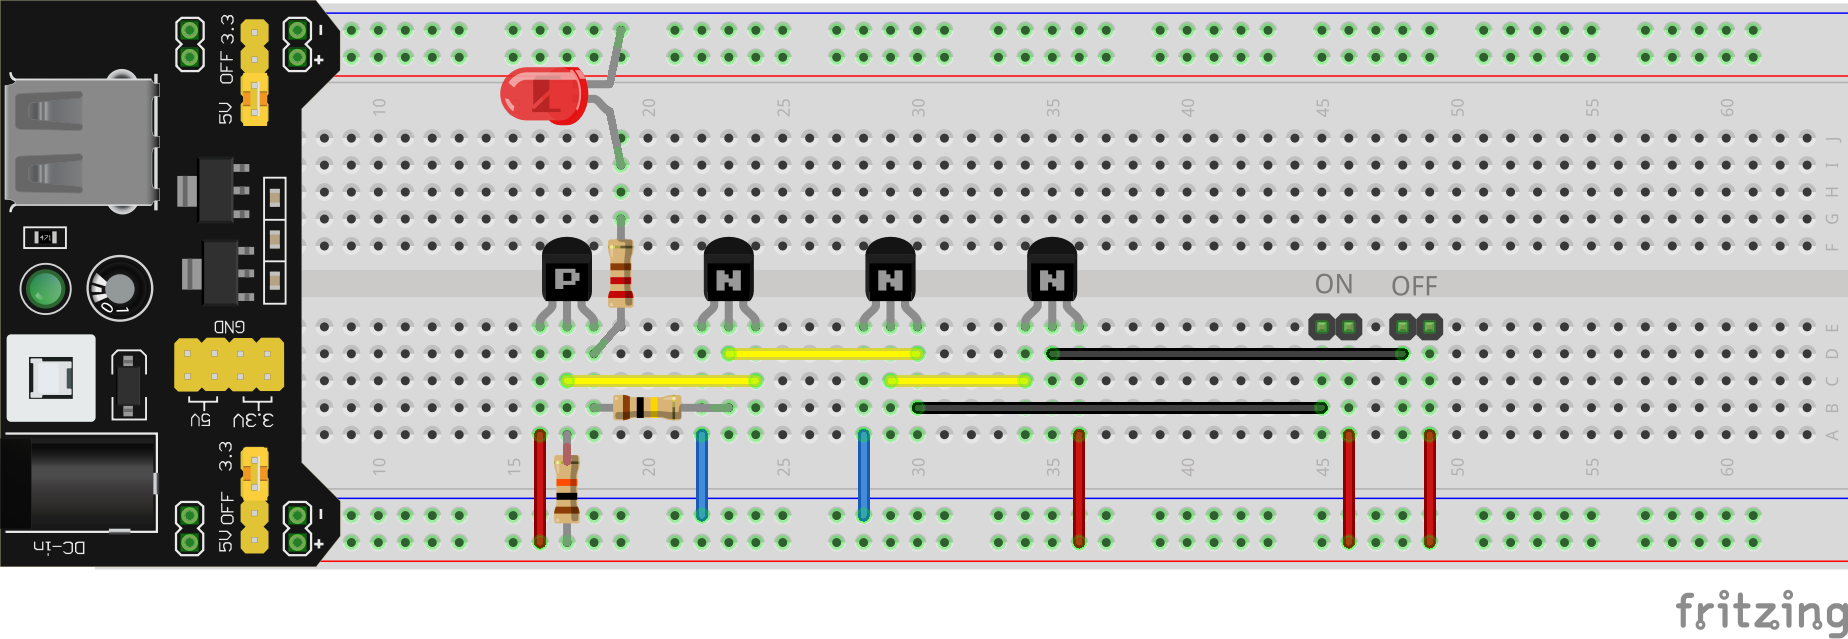
\includegraphics[width=\textwidth]{lesson_circuits/L7/lesson_7.png}
    \caption{On/Off touch switch using BJTs Breadboard Schematic}
    \label{fig:onoff_sch}
\end{figure}
\begin{figure}[!htp]
    \centering
    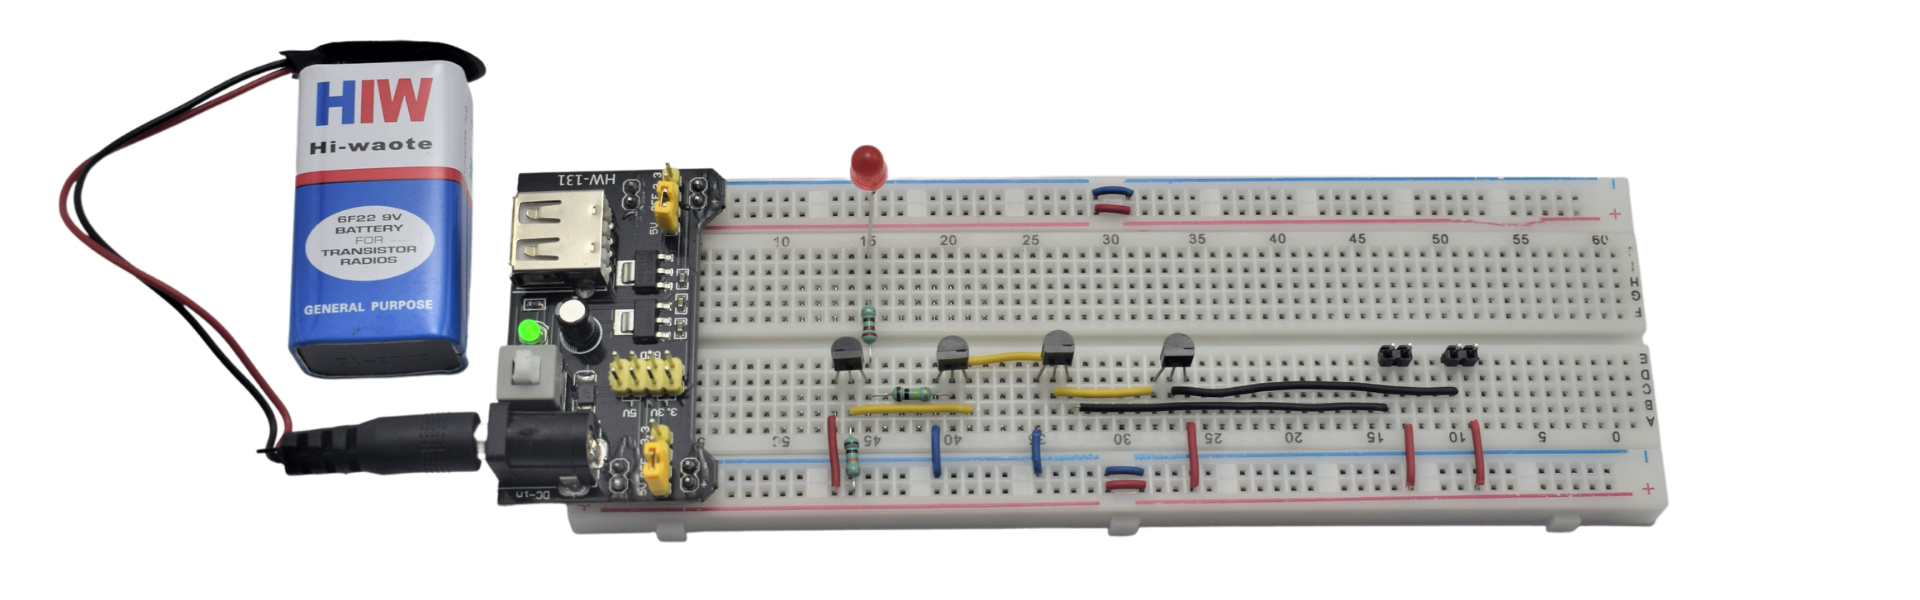
\includegraphics[width=\textwidth]{lesson_circuits/L7/L7-A.png}
    \caption{On/Off Touch Switch: }
    \label{fig:onoff_obb1}
\end{figure}
\begin{figure}[!htp]
    \centering
    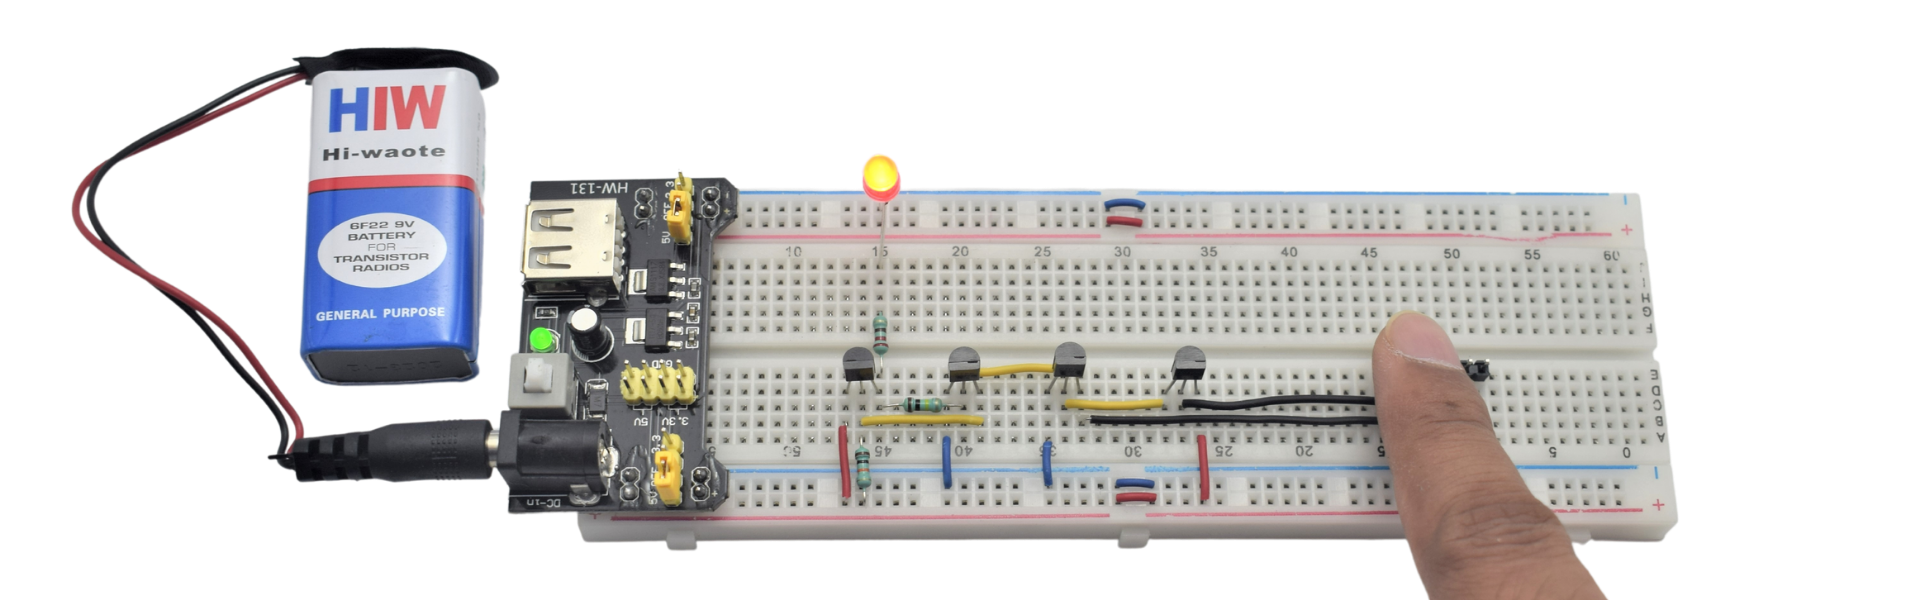
\includegraphics[width=\textwidth]{lesson_circuits/L7/L7-B.png}
    \caption{On/Off Touch Switch: }
    \label{fig:onoff_obb2}
\end{figure}
\begin{figure}[!htp]
    \centering
    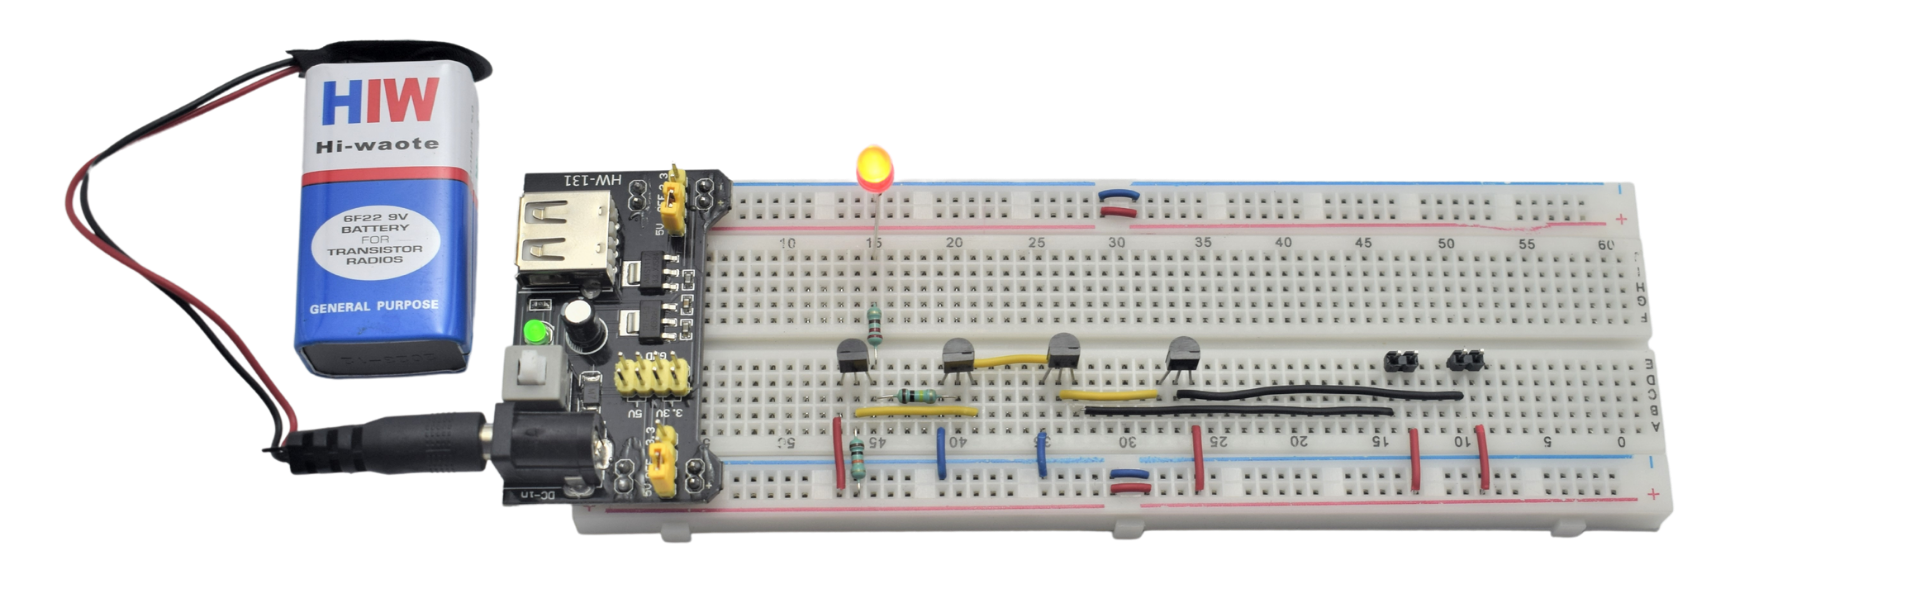
\includegraphics[width=\textwidth]{lesson_circuits/L7/L7-C.png}
    \caption{On/Off Touch Switch: }
    \label{fig:onoff_obb3}
\end{figure}
\begin{figure}[!htp]
    \centering
    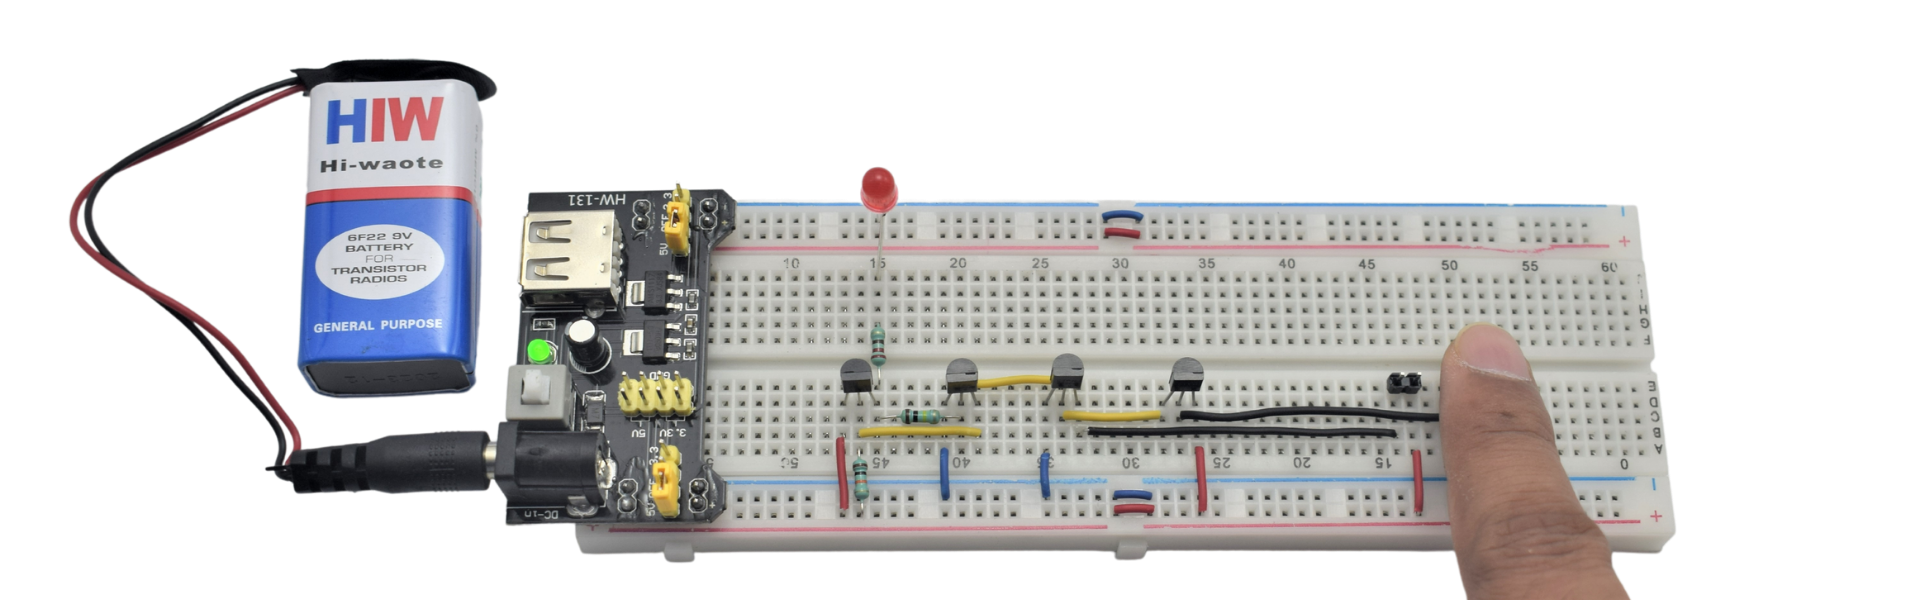
\includegraphics[width=\textwidth]{lesson_circuits/L7/L7-D.png}
    \caption{On/Off Touch Switch: }
    \label{fig:onoff_obb4}
\end{figure}
\begin{figure}[!htp]
    \centering
    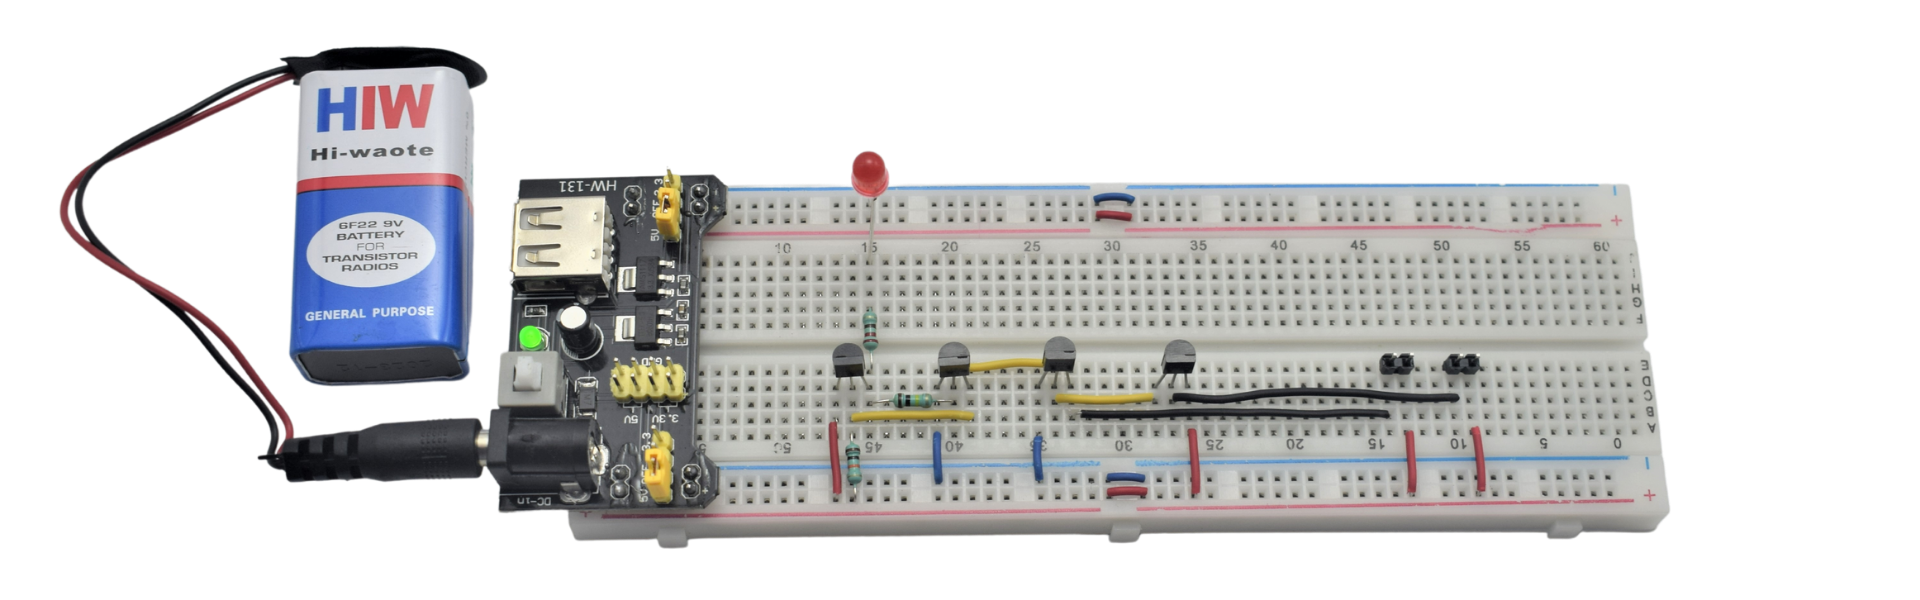
\includegraphics[width=\textwidth]{lesson_circuits/L7/L7-E.png}
    \caption{On/Off Touch Switch: }
    \label{fig:onoff_obb5}
\end{figure}


\section{Lesson 8: Toggle Switch using Transistors}
\subsection{Objective}
In this activity we will make an toggle switch which toggles the output state using push button and transistors.
\subsection{Components Required}
\begin{enumerate}
    \item Breadboard Power Supply $\times$ 1
    \item 9V Battery $\times$ 1
    \item 9V Battery Connector $\times$ 1
    \item Breadboard $\times$ 1
    \item Red LED $\times$ 1
    \item \SI{100}{\nano\farad} $\times$ 1
    \item \SI{220}{\ohm} $\times$ 1
    \item \SI{10}{\kilo\ohm} $\times$ 1
    \item \SI{100}{\kilo\ohm} $\times$ 2
    \item \SI{1}{\mega\ohm} $\times$ 2
    \item 2N2222 NPN Transistor $\times$ 2
    \item 2N2907 PNP Transistor $\times$ 1
    \item 10-XX Push Button $\times$ 1
    \item Male-Male jumper wire $\times$ 10
\end{enumerate}
\subsection{Circuit}
\begin{figure}[!htp]
    \centering
    \begin{circuitikz}[scale = 2]
        \draw (0,2.5) node[npn](t2){T2};
        \draw (2,3) node[pnp](t1){T1};
        \draw (-1.5,1) node[npn, xscale=-1](t3){\scalebox{-1}[1]{T3}};
        \draw (t2.E) to[short, -*] (0,0)
                node[ground](gnd1){};
        \draw (gnd1) -- (2,0)
                to[empty led, invert, mirror] ++(0,1)
                to[R, l_=$\SI{220}{\ohm}$] ++(0,0.7)
                to[short, -*] ++(0,0.2) -- (t1.C);
        \draw[red] (t1.E) -- ++(0,0.5)
                to[short, -*] ++(-2,0) node[vcc](vcc1){5V};
        \draw[red] (vcc1) -| ++(-1.5,-1.5)
                to[R, l=$\SI{1}{\mega\ohm}$] (t3.C);
        \draw (vcc1) to[R, l=$\SI{10}{\kilo\ohm}$] (t2.C);
        \draw[blue] (t1.B) to[short, -*] ++(-1.58,0);
        \draw[green] (t2.B) -- ++(-1,0)
                to[push button, mirror] (-3,2.5) -- ++(0,-1.1);
        \draw (t3.E) to[short, -*] (-1.5,0) -- (gnd1);
        \draw (-1.5,0) -- (-3,0);
        \draw (t3.C) to[short, *-] ++(0,0)
                to[R, l_=$\SI{1}{\mega\ohm}$] ++(-1.5,0)
                to[short, *-] ++(0,0)
                to[C, l=$\SI{100}{\nano\farad}$] (-3,0);
        \draw[orange] (t3.B) to[R, l=$\SI{100}{\kilo\ohm}$] ++(0.7,0) -- ++(2.1,0)
                to[short, -*] ++(0,0.9);
        \draw[purple] (t2.B) to[short, *-] ++(0,-0.6)
                to[R, l=$\SI{100}{\kilo\ohm}$] (2,1.9);
    \end{circuitikz}
    \caption{Toggle Switch using Transistors}
    \label{fig:toggle_transistor}
\end{figure}
\subsection{Circuit Explanation}
Let us assume that initially all the transistors are off along with the led. In this case, the capacitor gets charged via the two $1\si{\mega\ohm}$ resistors. And no current is flowing through any transistor.
\begin{figure}[!htp]
    \centering
    \begin{circuitikz}[scale = 2]
        \draw (0,2.5) node[npn](t2){T2};
        \draw (2,3) node[pnp](t1){T1};
        \draw (-1.5,1) node[npn, xscale=-1](t3){\scalebox{-1}[1]{T3}};
        \draw (t2.E) to[short, -*] (0,0)
                node[ground](gnd1){};
        \draw (gnd1) -- (2,0)
                to[empty led, invert, mirror] ++(0,1)
                to[R, l_=$\SI{220}{\ohm}$] ++(0,0.7)
                to[short, -*] ++(0,0.2) -- (t1.C);
        \draw[red] (t1.E) -- ++(0,0.5)
                to[short, -*] ++(-2,0) node[vcc](vcc1){5V};
        \draw[red] (vcc1) -| ++(-1.5,-1.5)
                to[R, l=$\SI{1}{\mega\ohm}$] (t3.C);
        \draw (vcc1) to[R, l=$\SI{10}{\kilo\ohm}$] (t2.C);
        \draw[blue] (t1.B) to[short, -*] ++(-1.58,0);
        \draw[green] (t2.B) -- ++(-1,0)
                to[push button, mirror] (-3,2.5) -- ++(0,-1.1);
        \draw (t3.E) to[short, -*] (-1.5,0) -- (gnd1);
        \draw (-1.5,0) -- (-3,0);
        \draw (t3.C) to[short, *-] ++(0,0)
                to[R, l_=$\SI{1}{\mega\ohm}$] ++(-1.5,0)
                to[short, *-] ++(0,0)
                to[C, l=$\SI{100}{\nano\farad}$] (-3,0);
        \draw[orange] (t3.B) to[R, l=$\SI{100}{\kilo\ohm}$] ++(0.7,0) -- ++(2.1,0)
                to[short, -*] ++(0,0.9);
        \draw[purple] (t2.B) to[short, *-] ++(0,-0.6)
                to[R, l=$\SI{100}{\kilo\ohm}$] (2,1.9);
        \draw[-latex, brown]
            ($(vcc1)+(-0.2,0.2)$) -- ++(-1.5,0) -- ++(0,-3) -- ++(-1.6,0) -- ++(0,-1);
    \end{circuitikz}
    \caption{Toggle Switch using Transistor - Idle}
    \label{fig:toggle_switch_bjt_idle}
\end{figure}

When we press the switch, the capacitor's +ve plate is connected to the base of the transistor $T2$, and therefore a base current starts flowing, turning $T2$ on. With $T2$ on the base of transistor $T1$ is pulled to ground, turning it and the led on. There is also a feedback current flowing back to base of $T2$ and $T3$.
\begin{figure}[!htp]
    \centering
    \begin{circuitikz}[scale = 2]
        \draw (0,2.5) node[npn](t2){T2};
        \draw (2,3) node[pnp](t1){T1};
        \draw (-1.5,1) node[npn, xscale=-1](t3){\scalebox{-1}[1]{T3}};
        \draw (t2.E) to[short, -*] (0,0)
                node[ground](gnd1){};
        \draw (gnd1) -- (2,0)
                to[empty led, invert, mirror] ++(0,1)
                to[R, l_=$\SI{220}{\ohm}$] ++(0,0.7)
                to[short, -*] ++(0,0.2) -- (t1.C);
        \draw[red] (t1.E) -- ++(0,0.5)
                to[short, -*] ++(-2,0) node[vcc](vcc1){5V};
        \draw[red] (vcc1) -| ++(-1.5,-1.5)
                to[R, l=$\SI{1}{\mega\ohm}$] (t3.C);
        \draw (vcc1) to[R, l=$\SI{10}{\kilo\ohm}$] (t2.C);
        \draw[blue] (t1.B) to[short, -*] ++(-1.58,0);
        \draw[green] (t2.B) -- ++(-1,0)
                to[normally closed push button, mirror] (-3,2.5) -- ++(0,-1.1);
        \draw (t3.E) to[short, -*] (-1.5,0) -- (gnd1);
        \draw (-1.5,0) -- (-3,0);
        \draw (t3.C) to[short, *-] ++(0,0)
                to[R, l_=$\SI{1}{\mega\ohm}$] ++(-1.5,0)
                to[short, *-] ++(0,0)
                to[C, l=$\SI{100}{\nano\farad}$] (-3,0);
        \draw[orange] (t3.B) to[R, l=$\SI{100}{\kilo\ohm}$] ++(0.7,0) -- ++(2.1,0)
                to[short, -*] ++(0,0.9);
        \draw[purple] (t2.B) to[short, *-] ++(0,-0.6)
                to[R, l=$\SI{100}{\kilo\ohm}$] (2,1.9);
        \draw[-latex, brown]
            (-3.2,1) -- ++(0,1.8) -- ++(2.8,0);
        \draw[-latex, red]
            (2.4, 3.8) -- (2.4, 0.2);
        \draw[<->, purple]
            (-0.3, 1.2) -- (1.6, 1.2) -- (1.6,1.6) -- ++(-2,0)
            node[midway, below=1mm]{feedback};
    \end{circuitikz}
    \caption{Toggle Switch using Transistor - On}
    \label{fig:toggle_switch_bjt_on}
\end{figure}

On leaving the switch, the feedback current keeps the $T2$ on which keeps $T1$ on. Also, this feedback current turn on the $T3$ which discharges the capacitor through it. At this stage all the transistors are on, led is on and the capacitor is completely discharged.
\begin{figure}[!htp]
    \centering
    \begin{circuitikz}[scale = 2]
        \draw (0,2.5) node[npn](t2){T2};
        \draw (2,3) node[pnp](t1){T1};
        \draw (-1.5,1) node[npn, xscale=-1](t3){\scalebox{-1}[1]{T3}};
        \draw (t2.E) to[short, -*] (0,0)
                node[ground](gnd1){};
        \draw (gnd1) -- (2,0)
                to[empty led, invert, mirror] ++(0,1)
                to[R, l_=$\SI{220}{\ohm}$] ++(0,0.7)
                to[short, -*] ++(0,0.2) -- (t1.C);
        \draw[red] (t1.E) -- ++(0,0.5)
                to[short, -*] ++(-2,0) node[vcc](vcc1){5V};
        \draw[red] (vcc1) -| ++(-1.5,-1.5)
                to[R, l=$\SI{1}{\mega\ohm}$] (t3.C);
        \draw (vcc1) to[R, l=$\SI{10}{\kilo\ohm}$] (t2.C);
        \draw[blue] (t1.B) to[short, -*] ++(-1.58,0);
        \draw[green] (t2.B) -- ++(-1,0)
                to[push button, mirror] (-3,2.5) -- ++(0,-1.1);
        \draw (t3.E) to[short, -*] (-1.5,0) -- (gnd1);
        \draw (-1.5,0) -- (-3,0);
        \draw (t3.C) to[short, *-] ++(0,0)
                to[R, l_=$\SI{1}{\mega\ohm}$] ++(-1.5,0)
                to[short, *-] ++(0,0)
                to[C, l=$\SI{100}{\nano\farad}$] (-3,0);
        \draw[orange] (t3.B) to[R, l=$\SI{100}{\kilo\ohm}$] ++(0.7,0) -- ++(2.1,0)
                to[short, -*] ++(0,0.9);
        \draw[purple] (t2.B) to[short, *-] ++(0,-0.6)
                to[R, l=$\SI{100}{\kilo\ohm}$] (2,1.9);
        \draw[-latex, brown]
            (-3.2,0.8) -- ++(0,1) -- ++(1.5,0) -- ++(0,-1.6);
        \draw[-latex, red]
            (2.4, 3.8) -- (2.4, 0.2);
        \draw[<->, purple]
            (-0.3, 1.2) -- (1.6, 1.2) -- (1.6,1.6) -- ++(-2,0)
            node[midway, below=1mm]{feedback};
    \end{circuitikz}
    \caption{Toggle Switch using Transistor - Idle On}
    \label{fig:toggle_switch_bjt_on_idle}
\end{figure}

Now, when we again press the switch, the feedback current going to base of $T2$, goes to ground via the capacitor, which is discharged and therefore provide little to no resistance. This turns off the $T2$, and the base of $T1$ is pulled back to $VCC$, causing it to turn off. Now the led is off and all the transistor are not conducting, which is idle state.
\begin{figure}[!htp]
    \centering
    \begin{circuitikz}[scale = 2]
        \draw (0,2.5) node[npn](t2){T2};
        \draw (2,3) node[pnp](t1){T1};
        \draw (-1.5,1) node[npn, xscale=-1](t3){\scalebox{-1}[1]{T3}};
        \draw (t2.E) to[short, -*] (0,0)
                node[ground](gnd1){};
        \draw (gnd1) -- (2,0)
                to[empty led, invert, mirror] ++(0,1)
                to[R, l_=$\SI{220}{\ohm}$] ++(0,0.7)
                to[short, -*] ++(0,0.2) -- (t1.C);
        \draw[red] (t1.E) -- ++(0,0.5)
                to[short, -*] ++(-2,0) node[vcc](vcc1){5V};
        \draw[red] (vcc1) -| ++(-1.5,-1.5)
                to[R, l=$\SI{1}{\mega\ohm}$] (t3.C);
        \draw (vcc1) to[R, l=$\SI{10}{\kilo\ohm}$] (t2.C);
        \draw[blue] (t1.B) to[short, -*] ++(-1.58,0);
        \draw[green] (t2.B) -- ++(-1,0)
                to[normally closed push button, mirror] (-3,2.5) -- ++(0,-1.1);
        \draw (t3.E) to[short, -*] (-1.5,0) -- (gnd1);
        \draw (-1.5,0) -- (-3,0);
        \draw (t3.C) to[short, *-] ++(0,0)
                to[R, l_=$\SI{1}{\mega\ohm}$] ++(-1.5,0)
                to[short, *-] ++(0,0)
                to[C, l=$\SI{100}{\nano\farad}$] (-3,0);
        \draw[orange] (t3.B) to[R, l=$\SI{100}{\kilo\ohm}$] ++(0.7,0) -- ++(2.1,0)
                to[short, -*] ++(0,0.9);
        \draw[purple] (t2.B) to[short, *-] ++(0,-0.6)
                to[R, l=$\SI{100}{\kilo\ohm}$] (2,1.9);
        \draw[-latex, brown]
            (-0.3,2.8) -- ++(-3,0) -- ++(0,-2);
        \draw[-latex, red]
            (2.4, 3.8) -- (2.4, 0.2);
        \draw[<->, purple]
            (-0.3, 1.2) -- (1.6, 1.2) -- (1.6,1.6) -- ++(-2,0)
            node[midway, below=1mm]{feedback};
    \end{circuitikz}
    \caption{Toggle Switch using Transistor - Off}
    \label{fig:toggle_switch_bjt_off}
\end{figure}
\subsection{Circuit Picture}
\begin{figure}[!htp]
    \centering
    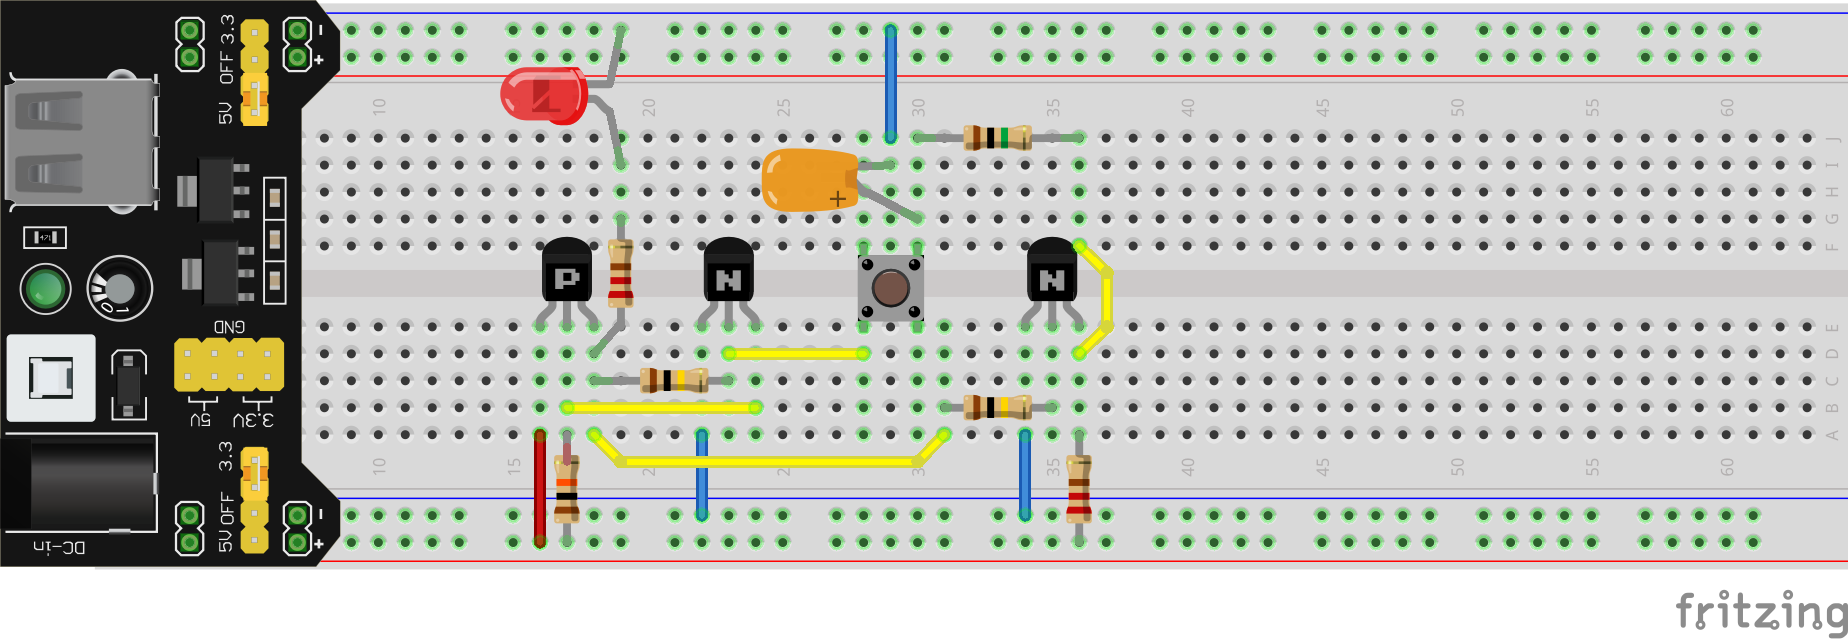
\includegraphics[width=\textwidth]{lesson_circuits/L8/lesson_8.png}
    \caption{Toggle Switch using BJTs Breadboard Schematic}
    \label{fig:toggle_bjt_sch}
\end{figure}
\begin{figure}[!htp]
    \centering
    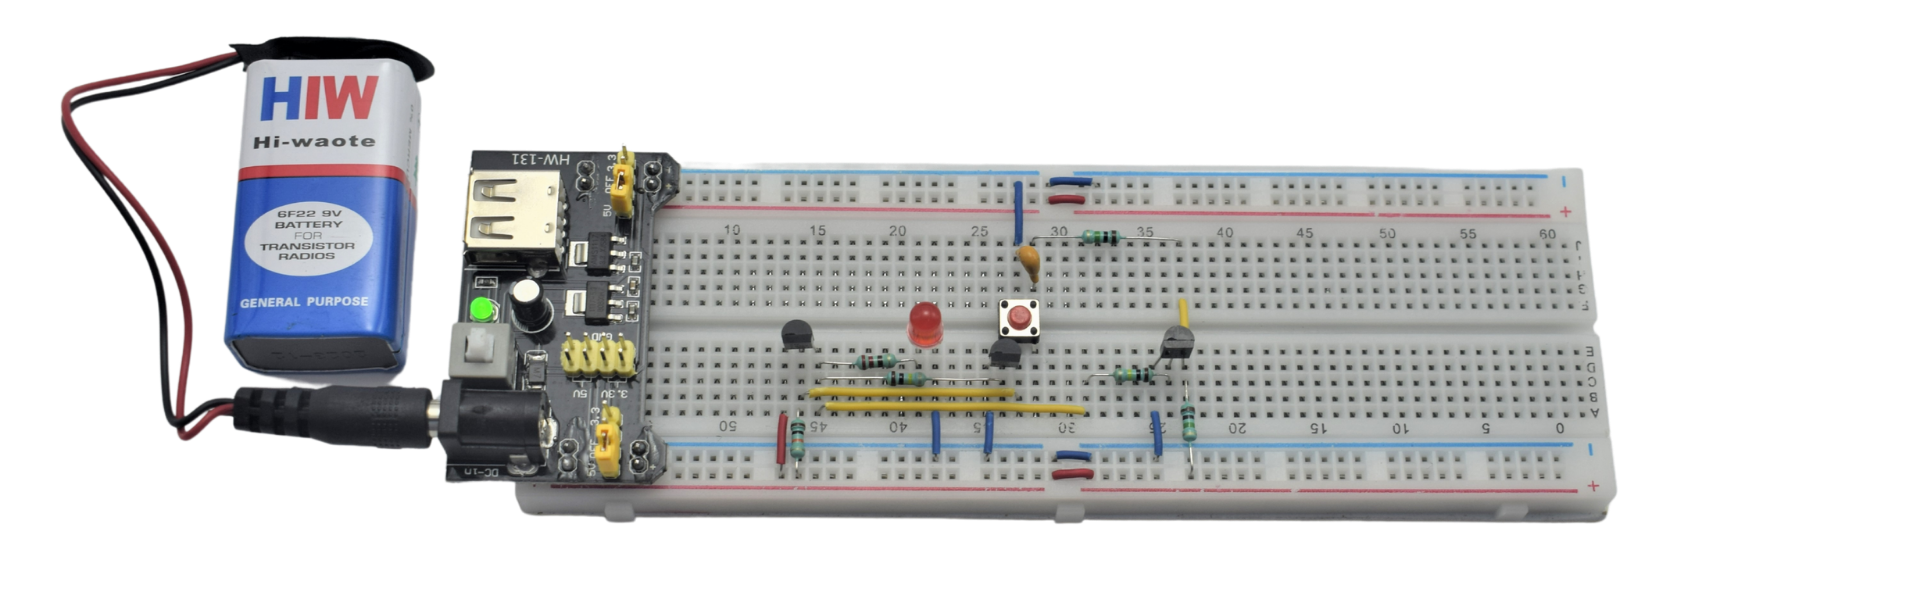
\includegraphics[width=\textwidth]{lesson_circuits/L8/L8-A.png}
    \caption{Toggle Switch: Off State}
    \label{fig:toggle_bjt_obb1}
\end{figure}
\begin{figure}[!htp]
    \centering
    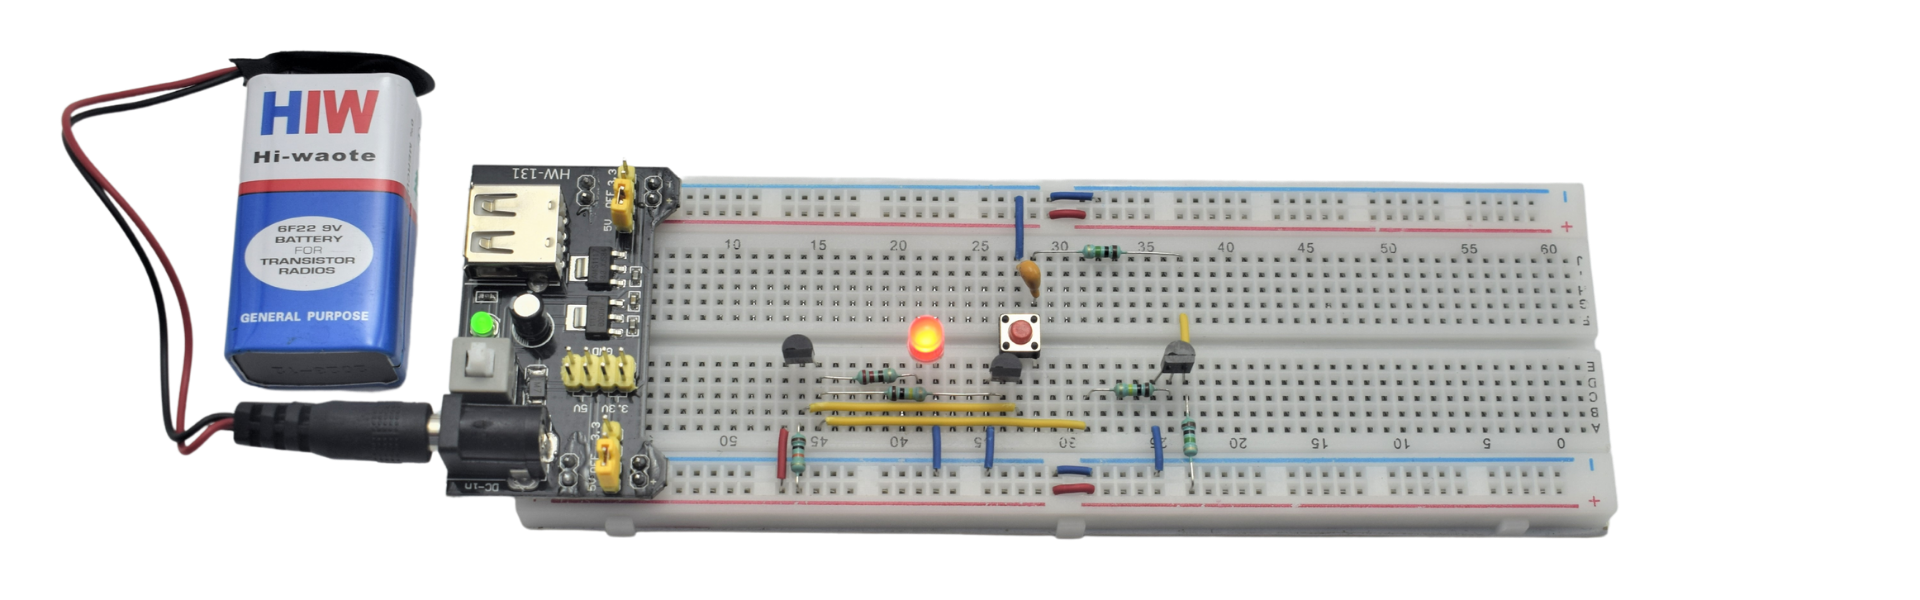
\includegraphics[width=\textwidth]{lesson_circuits/L8/L8-B.png}
    \caption{Toggle Switch: On State}
    \label{fig:toggle_bjt_obb2}
\end{figure}



\section{Lesson 9: Two Color LED Flasher using Transistors}
\subsection{Objective}
In this activity we will use the astable multivibrator to flash a rgb led.
\subsection{Components Required}
\begin{enumerate}
    \item Breadboard Power Supply $\times$ 1
    \item 9V Battery $\times$ 1
    \item 9V Battery Connector $\times$ 1
    \item Breadboard $\times$ 1
    \item RGB LED (Common Cathode) $\times$ 1
    \item \SI{220}{\ohm} $\times$ 2
    \item \SI{100}{\kilo\ohm} $\times$ 2
    \item 2N2222 NPN Transistor $\times$ 2
    \item \SI{10}{\micro\farad} $\times$ 2
    \item Male-Male jumper wire $\times$ 5
\end{enumerate}
\subsection{Circuit}
\begin{figure}[!htp]
    \centering
    \begin{circuitikz}[scale = 2]
        \draw (0,0) to[short, *-] (0,0) node[ground](gnd1){};
        \draw (0,0) to[full led, invert, color=green] (0,1);
        \draw (0,0) -- (0.5,0) to[full led, invert, color=red] (0.5,1);
        \draw (0,0) -- (-0.5,0) to[full led, invert, color=blue] (-0.5,1);
        \draw (-1.5,1.7) node[npn](t2){T2};
        \draw (1.5,1.7) node[npn, xscale=-1](t1){\scalebox{-1}[1]{T1}};
        \draw (t1.E) -| (0,1);
        \draw (t2.E) -| (-0.5,1);
        \draw (t1.C) to[short, -*] ++(0,0.5)
                to[R, l_=$\SI{220}{\ohm}$] ++(0,0.8)
                to[short, -*] ++(0,0.1) -- ++(1,0)
                to[R, l=$\SI{100}{\kilo\ohm}$] ++(0,-1)
                to[short, -*] ++(0,-0.2) |- (t1.B);
        \draw (t2.C) to[short, -*] ++(0,0.5)
                to[R, l=$\SI{220}{\ohm}$] ++(0,0.8)
                to[short, -*] ++(0,0.1) -- ++(-1,0)
                to[R, l_=$\SI{100}{\kilo\ohm}$] ++(0,-1)
                to[short, -*] ++(0,-0.4) |- (t2.B);
        \draw (-1.5, 3.48) to[short, -*] (0,3.48) node[vcc]{VCC}
                -- (1.5, 3.48);
        \draw ($(t2.C)+(0,0.5)$) to[C, l=$\SI{10}{\micro\farad}$] ++(1.3,0) 
                |- (2.5,2.28);
        \draw ($(t1.C)+(0,0.5)$) to[C, l_=$\SI{10}{\micro\farad}$] ++(-1.3,0) 
                |- (-2.5,2.08);
    \end{circuitikz}
    \caption{Two Color LED Flasher using Transistor}
    \label{fig:rgb_transistor}
\end{figure}
\subsection{Circuit Explanation}
This circuit operation is similar to that of astable multivibrator. Both the capacitors charge and discharge alternatively and thus turn on and off the transistors, causing the led to light up alternatively or in a flashing manner. By changing the capacitor and resistor values independently we can change the turn on and off time of both the LEDs.
\subsection{Circuit Picture}
\begin{figure}[!htp]
    \centering
    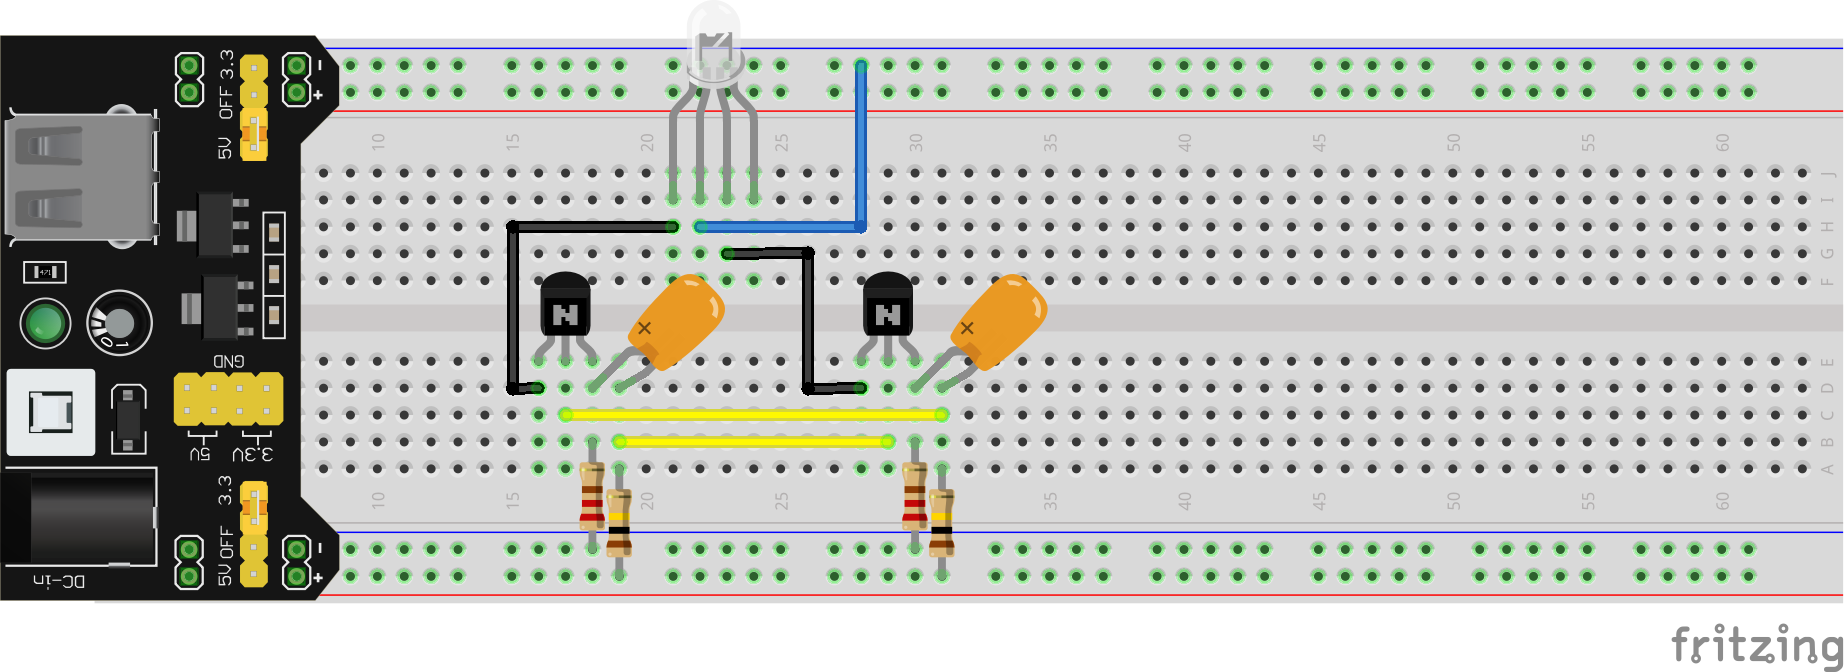
\includegraphics[width=\textwidth]{lesson_circuits/L9/lesson_9.png}
    \caption{Two Color LED flasher using BJTs Breadboard Schematic}
    \label{fig:two_led_bjt_sch}
\end{figure}
\begin{figure}[!htp]
    \centering
    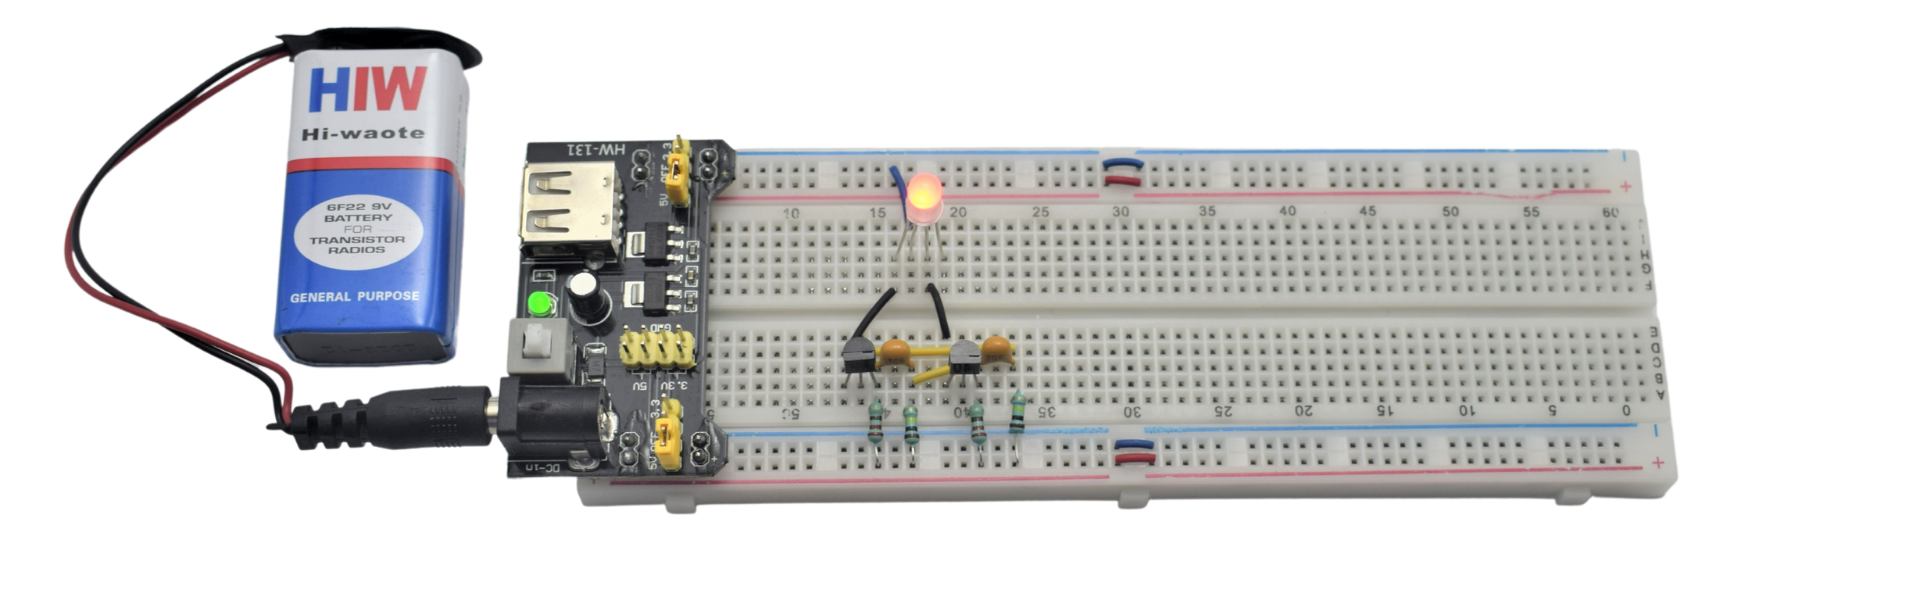
\includegraphics[width=\textwidth]{lesson_circuits/L9/L9-A.png}
    \caption{Two Color LED flasher}
    \label{fig:bjt_2led_obb}
\end{figure}



\section{Lesson 10: Light Sensitive LED using LDR}
\subsection{Objective}
In this activity we will make light sensitive LED, which will light up in darkness.
\subsection{Components Required}
\begin{enumerate}
    \item Breadboard Power Supply $\times$ 1
    \item 9V Battery $\times$ 1
    \item 9V Battery Connector $\times$ 1
    \item Breadboard $\times$ 1
    \item RGB LED (Common Cathode) $\times$ 1
    \item \SI{220}{\ohm} $\times$ 1
    \item \SI{100}{\kilo\ohm} $\times$ 1
    \item LDR (Photo-resistor) $\times$ 1
    \item Male-Male jumper wire $\times$ 3
\end{enumerate}
\subsection{Circuit}
\begin{figure}[!htp]
    \centering
    \begin{circuitikz}[scale = 2]
        \draw (0,0) node[ground](gnd1){};
        \draw (0,1) node[npn](t1){$T_1= 2N2222$};
        \draw (gnd1) -- ++(-1,0)
            to[sR,l=$LDR$] (-1,1)
            -- (t1.B);
        \draw (t1.C) to[empty led, invert, mirror] (0,2)
                to[R, l=$\SI{220}{\ohm}$] (0,3)
                node[vcc](vcc1){$V_cc$};
        \draw (vcc1) -| (-1,1) to[short, *-] ++(0,0);
        \draw (gnd1) -- (t1.E);
    \end{circuitikz}
    \caption{Light Sensitive LED}
    \label{fig:ldr_bjt_led}
\end{figure}
\subsection{Circuit Explanation}
We have used LDR in a voltage divider configuration. When there is change in light falling on the LDR, the voltage
drop across it will change due to change in it's resistance.
\begin{figure}[!htp]
    \centering
    \begin{circuitikz}[scale = 2]
        \draw (0,0) -- (-1,0)
            to[sR, l=$R_{LDR}$] (-1,1) node[](A){}
            to[R, l=$R_{fixed}$] (-1,2) -- (0,2);
        \draw[-latex]
            (A) to[short, *-] (0,1);
        \draw (-0.1,2.1) node[]{$V_{cc}$};
        \draw (-0.1,1.1) node[]{$V_{out}$};
        \draw (-0.1,0.1) node[]{$GND$};
    \end{circuitikz}
    \caption{LDR as Voltage Divider}
    \label{fig:ldr_volt_div}
\end{figure}

The output voltage ($V_{out}$) can be calculate by using the formula -
\begin{align*}
    V_{out} = V_{cc} \times \frac{R_{LDR}}{R_{LDR} + R_{fixed}}
\end{align*}
According to LDR data-sheet, we can find the threshold value of $R_{LDR}$ in dark and daylight, 
after that we need to find the value of $R_{fixed}$ such that the following conditions below are met -
\begin{enumerate}
    \item $0.7\si{\volt} \leq V_{out}$ in the dark.
    \item $0.7\si{\volt} > V_{out}$ in the daylight.
    \item The base current should be more than 20\si{\uA}
\end{enumerate}

In dark, $R_{LDR} = 550\si{\kohm}$ and in daylight, $R_{LDR} = 6\si{\kohm}$.

Let's work out each condition one by one.

\emph{The first condition}
\begin{align*}
    0.7\si{\V} & \leq V_{out} \\
    V_{out} & \leq V_{cc} \times \frac{R_{LDR}}{R_{LDR} + R_{fixed}} \\
    0.7\si{\V} & \leq 5\si{\V} \times \frac{550\si{\kohm}}{550\si{\kohm} +  R_{fixed}} \\
    R_{fixed} + 550\si{\kohm} & \leq \frac{5}{0.7} \times 550\si{kohm} \\
    R_{fixed} & \leq 3928.57\si{\kohm} - 550\si{\kohm} \\
    R_{fixed} & \leq 3.38\si{\Mohm} \\
\end{align*}

\emph{The second condition}
\begin{align*}
    0.7\si{\V} & > V_{out} \\
    V_{out} & > V_{cc} \times \frac{R_{LDR}}{R_{LDR} + R_{fixed}} \\
    0.7 & > 5\si{\V} \times \frac{6\si{\kohm}}{6\si{\kohm} + R_{fixed}} \\
    R_{fixed} + 6\si{\kohm} & > \frac{5}{0.7} \times 6\si{\kohm} \\
    R_{fixed} & > 42.86\si{\kohm} - 6\si{\kohm} \\
    R_{fixed} & > 36.86\si{\kohm} \\
\end{align*}

\emph{The third condition}
\begin{align*}
    V_{cc} & > 0.7\si{\V} + R_{fixed} \times I \\
    R_{fixed} & < \frac{5 - 0.7}{20\si{\uA}} \\
    R_{fixed} & < 215\si{\kohm} \\
\end{align*}

Now, analyzing all the above three conditions we see that - 
\begin{align*}
    36.86\si{\kohm} < R_{fixed} < 215\si{\kohm}
\end{align*}

We have selected $R_{fixed} = 100\si{\kohm}$.

\subsection{Circuit Picture}
\begin{figure}[!htp]
    \centering
    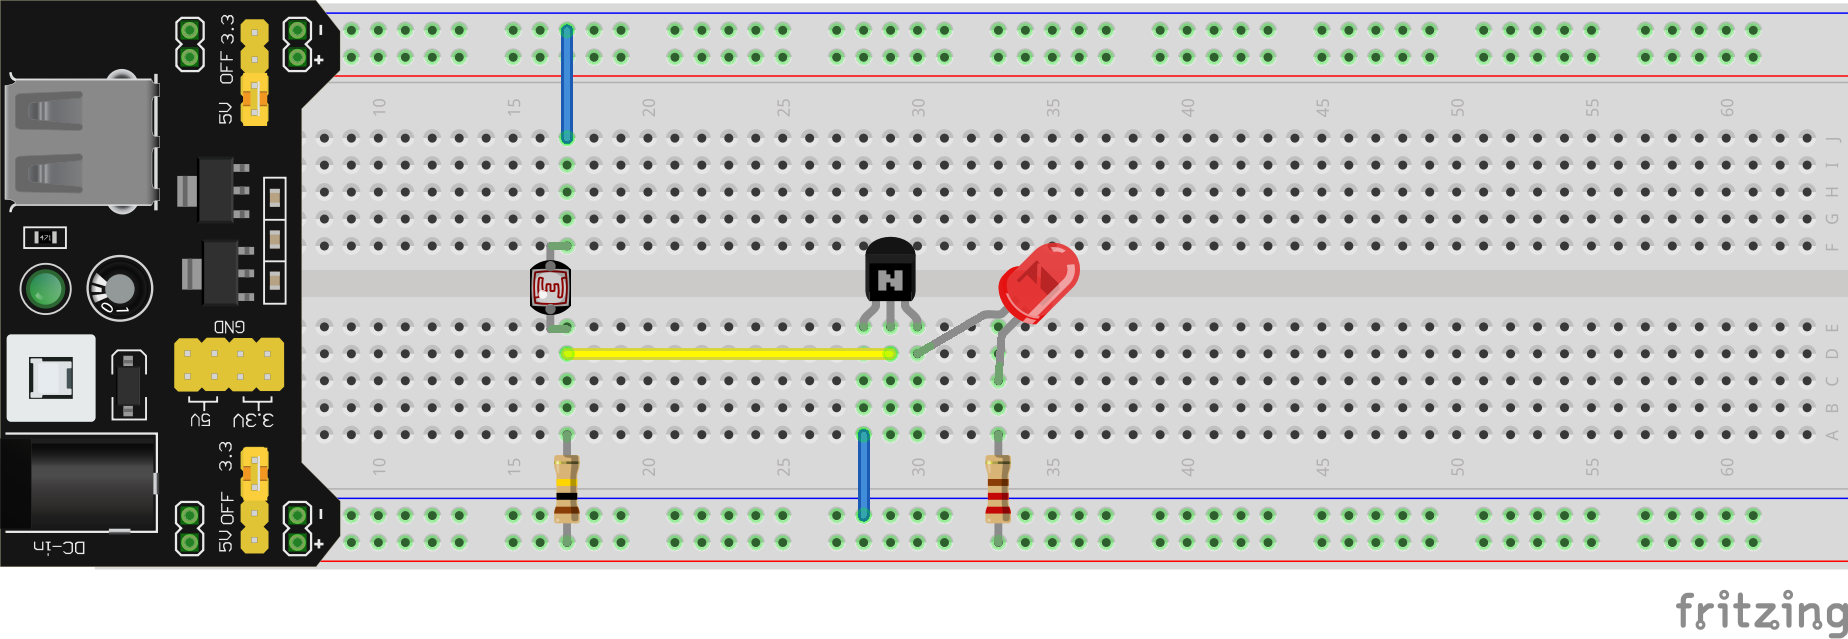
\includegraphics[width=\textwidth]{lesson_circuits/L10/lesson_10.png}
    \caption{Light sensitive LED Breadboard Schematic}
    \label{fig:light_sense_bjt_sch}
\end{figure}
\begin{figure}[!htp]
    \centering
    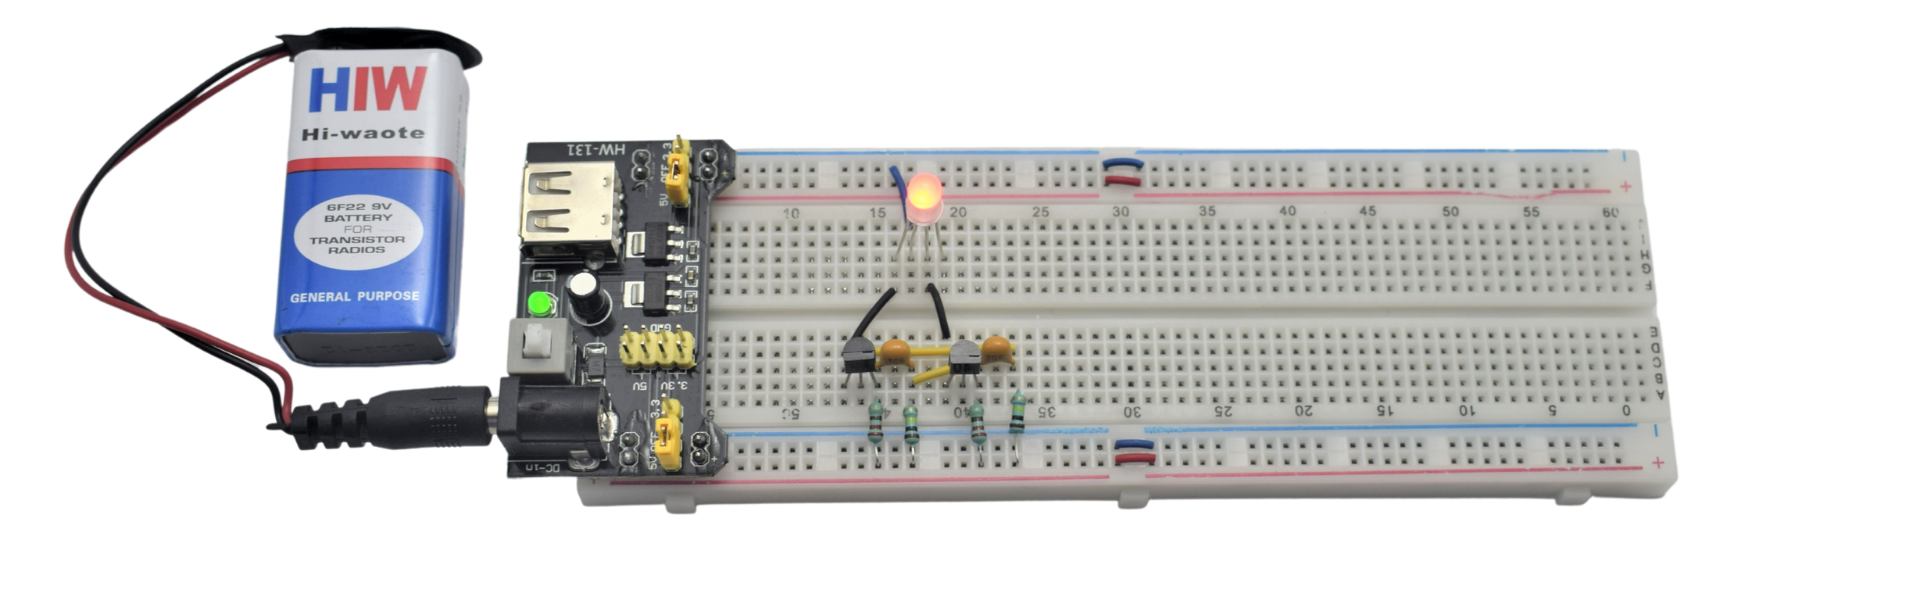
\includegraphics[width=\textwidth]{lesson_circuits/L9/L9-A.png}
    \caption{Light sensitive LED}
    \label{fig:ldr_bjt_working_obb}
\end{figure}
%----------------------------------------------------------------------------------------
%	CHAPTER 4
%----------------------------------------------------------------------------------------
\cleardoublepage
\chapterimage{chap_head.png} % Chapter heading image

\chapter{555}

\section{Overview}
In this section you'll learn about one of the most famous integrated circuit (IC) in use. Each year millions of 555 Timer ICs are manufactured and sold.
It's named 555 because there are three \SI{5}{\kilo\ohm} resistors inside the IC. And as the name suggest, it is a timer circuit. 
The timing interval is controlled by an external resistor/capacitor network. And by changing the values for the resistor and 
capacitor the timing duration can be easily varied.

Let's take a look at the pins of 555 Timer IC:
\begin{enumerate}
    \item \textbf{GND - Pin 1} Ground pin of the IC
    \item \textbf{VCC - Pin 8} Positive supply is connected to this pin, the voltage must be at least \SI{4.5}{\volt} and maximum \SI{15}{\volt}.
    \item \textbf{OUT - Pin 3} The output is either low (close to \SI{0}{\volt}) or high (close to VCC).
    \item \textbf{TRG - Pin 2} Trigger is active low, which means when the voltage on this pin drops below one-third of the supply voltage, the output of 555 goes high.
    \item \textbf{DIS - Pin 7} This pin is used to discharge an external capacitor that works in conjunction with a resistor to control the timing of the 555 IC.
    \item \textbf{THR - Pin 6} Threshold pin is used to monitor the voltage across the capacitor that's discharged by pin 7. When this voltage reaches two-third of the supply voltage, the output goes low.
    \item \textbf{CTRL - Pin 5} Control pin can be used to vary the voltage level at the inverting input of the threshold comparator. It is generally connected to ground via \SI{0.01}{\micro\farad} capacitor to eliminate any fluctuation on noise in the operation of the timer.
    \item \textbf{RST - Pin 4} Reset pin is active low, which means when this pin is momentarily grounded the 555 timer will reset it's state and will stop until it is triggered again.
\end{enumerate}

\begin{figure}[!htp]
    \centering
    \begin{circuitikz}[scale = 1.2]
        \draw (0,0) to [short, *-] (4.5,0) {};
        \draw (4.5,0) node[npn, anchor=E, rotate=-90, color=red](npn1){};
        \draw (npn1.C) to [short, -o] (7,0){} node[above=1mm]{DIS} node[below=1mm]{7};
        \draw (0,0) node[ground]{};
        \draw (0,0) 
            to [R, l=\SI{5}{\kilo\ohm}, color=blue] (0,1.8)
            to [R, l=\SI{5}{\kilo\ohm}, color=blue] (0, 3.6)
            to [R, l=\SI{5}{\kilo\ohm}, color=blue] (0, 5.4);
        \draw (-0.2,5.4) -- node[anchor=south, color=red] {VCC} (0.2,5.4);
        \draw (1.2,1.8) node[op amp, color=red](opamp1){};
        \draw (1.2,3.6) node[op amp, color=red](opamp2){};
        \draw 
            (opamp1.+) to [short, -*] ++(-0.4,0){}
            (opamp2.-) to [short, -*] ++(-0.4,0){} 
                to [short, -o] ++(-1,0)
                node[above=0.2mm]{CTRL} node[below=0.2mm]{5};
        \draw
            (opamp1.-) to [crossing] ++(-0.8,0) to[short, -o] ++(-0.6,0) 
            node[above=0.2mm]{TRG} node[below=0.2mm]{2}
            (opamp2.+) to [crossing] ++(-0.8,0) to[short, -o] ++(-0.6,0)
            node[above=0.2mm]{THR} node[below=0.2mm]{6};
        \draw (3.5,2.7) node[flipflop sr-rst, external pins width=0] (SR1){};
        \draw 
            (SR1.pin 1) -| (opamp2.out)
            (SR1.pin 3) -| (opamp1.out)
            (SR1.up) -- ++(0,1) 
            to [short,-o] ++(0,1) 
            node[left=1mm]{\ctikztextnot{RST}} node[right=1mm]{4};
        \draw 
            let 
                \p1 = (npn1.B),
                \p2 = (SR1.pin 6)
            in 
                (SR1.pin 6) to [short, -*] (\x1, \y2){}
                (npn1.B) -- (\x1, \y2){}
                (\x1, \y2) to[inline not] ++(2,0) 
                to[short, -o] ++(0,0) node[above=1mm]{OUT} node[below=1mm]{3};
        %\draw (SR1.pin 6) to [short, -*] ++(1,0) coordinate(nin);
        %\draw (npn1.B) -- (nin);
        %\draw (nin) to[inline not] ++(2,0);
    \end{circuitikz}
    \caption{555 Timer Circuit}
    \label{fig:555_internal_circuit}
\end{figure}

Figure \ref{fig:555_symbol} shows the schematic symbol for 555 IC that we will use in this chapter's circuit examples.
\begin{figure}[!htp]
    \centering
    \begin{circuitikz}[scale = 1.2]
        \TIMER555(0,0){1}
    \end{circuitikz}
    \caption{555 Timer Symbol}
    \label{fig:555_symbol}
\end{figure}

\section{555 : Working}
To understand how 555 timer IC works, let's look at the figure \ref{fig:555_internal_circuit}. The voltage at the negative input of 
the upper comparator is $\frac{2V_{cc}}{3}$ and the voltage at the positive input of the lower comparator is $\frac{V_{cc}}{3}$. 
So, whenever the voltage at TRG or pin 2 of 555 IC is below $\frac{V_{cc}}{3}$, the output of lower comparator is high, setting 
the flip flop, and therefore making the output high and turning off the internal transistor. Just like this, if the voltage at 
the pin 6 or THR goes above $\frac{2V_{cc}}{3}$ the upper comparator output goes high, it resets the flip flop and thus turning 
the output low while turning on the internal transistor.
\begin{figure}[!ht]
    \centering
    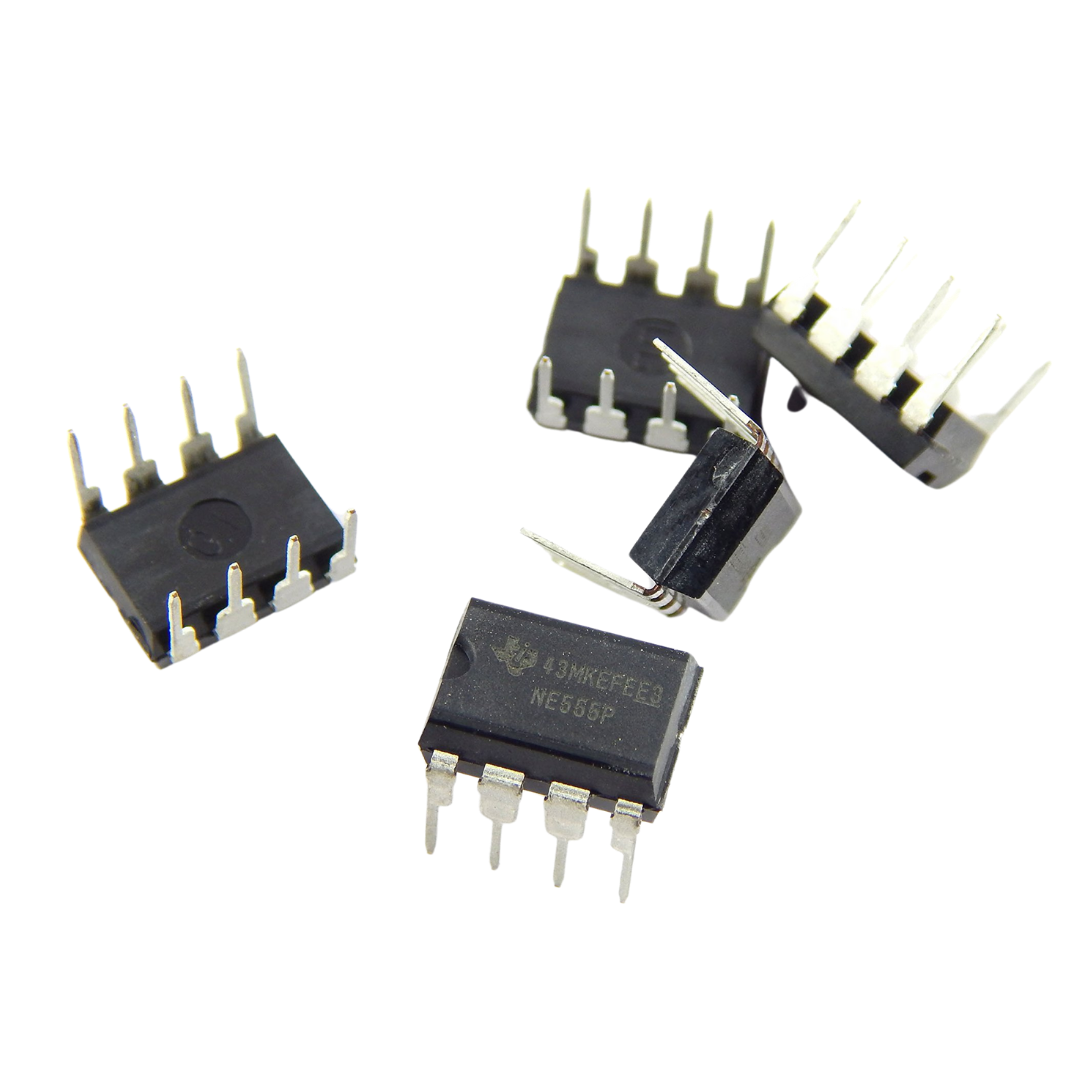
\includegraphics[width=0.8\textwidth]{Components/555.png}
    \caption{555 Timer IC}
    \label{fig:555_code}
\end{figure}
\subsection{Modes of Operations}
The 555 timer has 3 modes of operation and all of the upcoming activities utilizes one or more operation modes of 555.
In this section we will learn how to use different modes of operation of 555, after that we will build circuits using these modes.
\subsection{Astable Mode}\label{astablemode}
As the name suggests, in astable mode there is no stable state. The output continuously switches between high and low producing an
square wave. This circuit can be used for turning an LED on and off at regular intervals or act as a clock input for digital ICs
or control a motor by switching it on and off at regular time period.
\subsubsection{555 Astable Multivibrator Circuit}
\begin{figure}[!htp]
    \centering
    \begin{circuitikz}[scale = 1.2]
        \TIMER555(0,0){1}
        \draw (1 GND) to[short, -*] ++(0,-0.7) node[ground](g1){};
        \draw (1 CTRL) to[C, l=$C_{c}$] ++(0,-0.5) |- (g1);
        \draw (1 VCC) to[short, -*] ++(0,0.5) node[vcc](v1){$V_{cc}$};
        \draw (1 RESET) |- (v1);
        \draw (1 THR) to[short, -*] ++(-0.5,0) node[](s6){};
        \draw (1 TRG) to[short, -*] ++(-0.5,0) node[](s2){};
        \draw (1 DIS) to[short, -*] ++(-0.5,0) node[](s7){};
        \draw (s7) to[R, l_=$R_2$] ($(1 THR)-(0.5,0)$);
        \draw (s7) to[R, l=$R_1$] ++(0,1.5) |- (v1);
        \draw (s6) -- (s2) to[C, l_=$C$] ++(0,-1.5) |- (g1);
        \draw[-latex] (1 OUT) -- ++(0.5,0) node[above](o1){OUT};
        \draw ($(o1)+(0.5,0)$) -- ++(0.5,0) node[](w1){} -- ++(0,0.5) node[](t1){} -- ++(0.5,0) 
            -- ++(0,-0.5) node[](w2){} -- ++(0.5,0) node[](w3){} -- ++(0,0.5) node[](t2){} 
            -- ++(0.5,0) -- ++(0,-0.5) -- ++(0.5,0) -- ++(0,0.5) -- ++(0.5,0) -- ++(0,-0.5) -- ++(0.5,0);
        \draw[<->] ($(w1)-(0,0.1)$) -- ($(w2)-(0,0.1)$) node[midway, below](){$t_h$};
        \draw[<->] ($(w2)-(0,0.1)$) -- ($(w3)-(0,0.1)$) node[midway, below](){$t_l$};
        \draw[<->] ($(t1)+(0,0.1)$) -- ($(t2)+(0,0.1)$) node[midway, above](){$T$};
    \end{circuitikz}
    \caption{555 as Astable Multivibrator}
    \label{fig:555_astable}
\end{figure}

In astable configuration, both pin 2 (TRIG) and pin 6 (THR) are connected together, allowing the IC to re-trigger itself. This 
provides an oscillating output and the 555 works in an astable mode. When the power is turned on, the capacitor $C$ has zero 
charge and starts charging through resistors $R_1$ and $R_2$. The voltage at pin 2 and 6 is also 0, which makes the output of 
upper and lower comparator as shown in figure \ref{fig:555_internal_circuit} low and high, respectively. When the capacitor 
voltage reaches $\frac{2V_{cc}}{3}$, the upper comparator connected to pin 6 resets the flip flop making the output low 
and turning on the internal transistor.
\begin{figure}[!htp]
    \centering
    \begin{circuitikz}[scale = 1.2]
        \TIMER555(0,0){1}
        \draw (1 GND) to[short, -*] ++(0,-0.7) node[ground](g1){};
        \draw (1 CTRL) to[C, l=$C_{c}$] ++(0,-0.5) |- (g1);
        \draw (1 VCC) to[short, -*] ++(0,0.5) node[vcc](v1){$V_{cc}$};
        \draw (1 RESET) |- (v1);
        \draw (1 THR) to[short, -*] ++(-0.5,0) node[](s6){};
        \draw (1 TRG) to[short, -*] ++(-0.5,0) node[](s2){};
        \draw (1 DIS) to[short, -*] ++(-0.5,0) node[](s7){};
        \draw (s7) to[R, l_=$R_2$] ($(1 THR)-(0.5,0)$);
        \draw (s7) to[R, l=$R_1$] ++(0,1.5) |- (v1);
        \draw (s6) -- (s2) to[C, l_=$C$] ++(0,-1.5) |- (g1);
        \draw[-latex] (1 OUT) -- ++(0.5,0) node[above](o1){OUT};
        \draw ($(o1)+(0.5,0)$) -- ++(0.5,0) node[](w1){} -- ++(0,0.5) node[](t1){} -- ++(0.5,0) -- ++(0,-0.5) node[](w2){} -- ++(0.5,0) node[](w3){} -- ++(0,0.5) node[](t2){} -- ++(0.5,0) -- ++(0,-0.5) -- ++(0.5,0) -- ++(0,0.5) -- ++(0.5,0) -- ++(0,-0.5) -- ++(0.5,0);
        \draw[<->] ($(w1)-(0,0.1)$) -- ($(w2)-(0,0.1)$) node[midway, below](){$t_h$};
        \draw[<->] ($(w2)-(0,0.1)$) -- ($(w3)-(0,0.1)$) node[midway, below](){$t_l$};
        \draw[<->] ($(t1)+(0,0.1)$) -- ($(t2)+(0,0.1)$) node[midway, above](){$T$};
        \draw[-latex, red]
            ($(v1)+(-0.2,0.2)$) -- ++(-2.9,0) -- ++(0,-6);
    \end{circuitikz}
    \caption{555 as Astable Multivibrator : Capacitor Charging}
    \label{fig:555_astable_ccharg}
\end{figure}


When the internal transistor is turned on it starts discharging the capacitor through resistor $R_2$ as shown in the figure \ref{fig:555_astable_discharge}, 
now the capacitor starts discharging from $\frac{2V_{cc}}{3}$ towards 0 and when it reaches $\frac{V_{cc}}{3}$ the output of lower 
comparator goes high, setting the flip flop, making the output high and turning off the internal transistor. Now, the transistor is 
off the capacitor again starts charging and the same cycle repeats itself continuously until power is removed or reset pin is pulled low.
\begin{figure}[!htp]
    \centering
    \begin{circuitikz}[scale = 1.2]
        \TIMER555(0,0){1}
        \draw (1 GND) to[short, -*] ++(0,-0.7) node[ground](g1){};
        \draw (1 CTRL) to[C, l=$C_{c}$] ++(0,-0.5) |- (g1);
        \draw (1 VCC) to[short, -*] ++(0,0.5) node[vcc](v1){$V_{cc}$};
        \draw (1 RESET) |- (v1);
        \draw (1 THR) to[short, -*] ++(-0.5,0) node[](s6){};
        \draw (1 TRG) to[short, -*] ++(-0.5,0) node[](s2){};
        \draw (1 DIS) to[short, -*] ++(-0.5,0) node[](s7){};
        \draw (s7) to[R, l_=$R_2$] ($(1 THR)-(0.5,0)$);
        \draw (s7) to[R, l=$R_1$] ++(0,1.5) |- (v1);
        \draw (s6) -- (s2) to[C, l_=$C$] ++(0,-1.5) |- (g1);
        \draw[-latex] (1 OUT) -- ++(0.5,0) node[above](o1){OUT};
        \draw ($(o1)+(0.5,0)$) -- ++(0.5,0) node[](w1){} -- ++(0,0.5) node[](t1){} -- ++(0.5,0) -- ++(0,-0.5) node[](w2){} -- ++(0.5,0) node[](w3){} -- ++(0,0.5) node[](t2){} -- ++(0.5,0) -- ++(0,-0.5) -- ++(0.5,0) -- ++(0,0.5) -- ++(0.5,0) -- ++(0,-0.5) -- ++(0.5,0);
        \draw[<->] ($(w1)-(0,0.1)$) -- ($(w2)-(0,0.1)$) node[midway, below](){$t_h$};
        \draw[<->] ($(w2)-(0,0.1)$) -- ($(w3)-(0,0.1)$) node[midway, below](){$t_l$};
        \draw[<->] ($(t1)+(0,0.1)$) -- ($(t2)+(0,0.1)$) node[midway, above](){$T$};
        \draw[<-, blue]
            ($(1 DIS)-(0.1,0.1)$) -- ++(-1,0) -- ++(0,-4);
    \end{circuitikz}
    \caption{555 as Astable Multivibrator : Capacitor Discharging}
    \label{fig:555_astable_discharge}
\end{figure}

The time taken by the capacitor to discharge from $\frac{2V_{cc}}{3}$ to $\frac{V_{cc}}{3}$ is 
\begin{align*}
    t_l &= R_2 \dot C \dot ln(2) \\
    t_l &= 0.693R_2C \\
\end{align*}
and the charging time of capacitor from $\frac{V_{cc}}{3}$ to $\frac{2V_{cc}}{3}$ is 
\begin{align*}
    t_h &= (R_1 + R_2) \dot C \dot ln(2) \\
    t_h &= 0.693(R_1 + R_2)C \\
\end{align*}
The total time period and duty cycle of the output wave can know be determined using the equations 
\begin{align*}
    T &= t_l + t_h \\
    T &= 0.693R_2C + 0.693(R_1 + R_2)C \\
    T &= 0.693(R_1 + 2R_2)C \\
    D &= \frac{t_h}{t_h + t_l} \\
    D &= \frac{0.693(R_1 + R_2)}{0.693(R_1 + 2R_2)} \\
    D &= \frac{R_1 + R_2}{R_1 + 2R_2} \\
\end{align*}
We can change the frequency or time period and duty cycle of the output by selecting the appropriate values of $R_1$, $R_2$ and 
$C$.

\subsection{Monostable Mode}\label{monostable}
Monostable means only one stable state. In this mode 555 has only one stable state and can produce a pulse of set duration as a 
response against a trigger. The output stays low (the stable state) as long as there is no trigger received by the 555. Once, a
trigger event happens, the output momentarily goes to high and then falls back to low after a set duration. This circuit can be 
used to provide a delay pulse, or turn on LED or motor or any mechanism for a fixed duration of time.
\begin{figure}[!htp]
    \centering
    \begin{circuitikz}[scale = 1.2]
        \TIMER555(0,0){1}
        \draw (1 GND) to[short, -*] ++(0,-0.7) node[ground](g1){};
        \draw (1 CTRL) to[C, l=$C_{c}$] ++(0,-0.5) |- (g1);
        \draw (1 VCC) to[short, -*] ++(0,0.5) node[vcc](v1){$V_{cc}$};
        \draw (1 RESET) |- (v1);
        \draw (1 THR) to[short, -*] ++(-0.5,0) node[](s6){};
        \draw[->] (1 TRG) -- ++(-1.5,0) node[above](s2){Input};
        \draw (1 DIS) to[short, -*] ++(-0.5,0) node[](s7){};
        \draw (s7) -- ($(1 THR)-(0.5,0)$);
        \draw (s7) to[R, l=$R_1$] ++(0,1.5) |- (v1);
        \draw (s6) -- ++(0,-1) to[C, l_=$C$] ++(0,-1.7) |- (g1);
        \draw[-latex] (1 OUT) -- ++(0.5,0) node[above](o1){OUT};
        \draw ($(o1)+(0.5,1)$)node[above](){Input} -- ++(0.5,0) 
            -- ++(0,-0.5) -- ++(0.3,0) -- ++(0,0.5) -- ++(2,0);
        \draw ($(o1)+(0.5,-1)$)node[above](){Output} -- ++(0.5,0)
            -- ++(0,0.5) -- ++(1,0) -- ++(0,-0.5) -- ++(1.3,0);
    \end{circuitikz}
    \caption{555 as Monostable Multivibrator}
    \label{fig:555_monostable}
\end{figure}

The monostable circuit is pretty simple, we have the trigger pin 2 connected to a switch or any other mechanism that can pull it 
high or low. On power on the capacitor has 0 charge and the output is set low, when the trigger pin goes low the capacitor gets 
discharged via the internal transistor and output is set high and the capacitor starts charging through resistor $R_1$. When the 
capacitor reaches the voltage $\frac{V_{cc}}{3}$, the output goes low and the capacitor gets discharged via the internal transistor.

\subsection{Bistable Mode}\label{bistablemode}
In Bistable mode the 555 has two stable states. When it receives a trigger input pulse, the output goes to high state and stays there 
until it receives a reset pulse, which makes the output fall back to low. This circuit is sometimes called as flip/flop also, because 
it can store the value of it's state for as long as the device is not reset or set.
\begin{figure}[!htp]
    \centering
    \begin{circuitikz}[scale = 1.2]
        \TIMER555(0,0){1}
        \draw (1 GND) to[short, -*] ++(0,-0.7) node[ground](g1){};
        \draw (1 CTRL) to[C, l=$C_{c}$] ++(0,-0.5) |- (g1);
        \draw (1 VCC) to[short, -*] ++(0,0.5) node[vcc](v1){$V_{cc}$};
        \draw (1 RESET) -- ++(0,0.2) -- ++(-3.5,0) -- ++(0,-3)
            to[short, -*] ++(-0.5,0)node[](br){} to[R] 
            ++(0,3.3)node[](j1){} |- (v1);
        \draw (1 TRG) to[short, -*] ++(-2,0)node[](bt){} 
            -- ++(0,1.2) to[R] ++(0,3.3) 
            to[short, -*] (j1);
        \draw (bt) to[push button, mirror, l_=TRIG] ++(0,-1.5) |- (g1);
        \draw (br) -- ++(0,-1.2) to[push button, l=RST] ++(0,-1.5) |- (g1);
        \draw[-latex] (1 OUT) -- ++(0.5,0) node[above](o1){OUT};
        \draw ($(o1)+(0.5,1.5)$)node[above](){TRIG} -- ++(0.5,0) 
            -- ++(0,-0.5) -- ++(0.3,0) -- ++(0,0.5) -- ++(2,0);
        \draw ($(o1)+(0.5,0.5)$)node[above](){RST} -- ++(1.5,0) 
            -- ++(0,-0.5) -- ++(0.3,0) -- ++(0,0.5) -- ++(1,0);
        \draw ($(o1)+(0.5,-1)$)node[above](){Output} -- ++(0.5,0)
            -- ++(0,0.5) -- ++(1,0) -- ++(0,-0.5) -- ++(1.3,0);
    \end{circuitikz}
    \caption{555 in Bistable Mode}
    \label{fig:555_bistable}
\end{figure}

The bistable configuration is very simple, the reset and trigger pins are pulled up and connected to push buttons. When the TRIG 
button is pressed the output goes high and stays high until the RST button is pressed.
\clearpage

\section{Lesson 11: 555 LED Flasher}
\subsection{Objective}
In this activity we'll flash an LED using astable 555 multivibrator circuit.
\subsection{Components Required}
\begin{enumerate}
    \item Breadboard Power Supply $\times$ 1
    \item 9V Battery $\times$ 1
    \item 9V Battery Connector $\times$ 1
    \item Breadboard $\times$ 1
    \item 555 IC $\times$ 1
    \item Red LED $\times$ 1
    \item \SI{220}{\ohm} $\times$ 1
    \item \SI{10}{\kilo\ohm} $\times$ 1
    \item \SI{100}{\kilo\ohm} $\times$ 1
    \item \SI{100}{\nano\farad} $\times$ 1
    \item \SI{10}{\micro\farad} $\times$ 1
    \item Male-Male jumper wire $\times$ 7
\end{enumerate}
\subsection{Circuit}
\begin{figure}[!htp]
    \centering
    \begin{circuitikz}[scale = 1.2]
        \TIMER555(0,0){1}
        \draw (1 GND) to[short, -*] ++(0,-0.7) node[ground](g1){};
        \draw (1 CTRL) to[C, l=$100\si{\nano\farad}$] ++(0,-0.5)
            to[short, -*] ++(0,-0.2)node[](ctr){} |- (g1);
        \draw (1 VCC) to[short, -*] ++(0,0.5) node[vcc](v1){$V_{cc}$};
        \draw (1 RESET) |- (v1);
        \draw (1 THR) to[short, -*] ++(-0.5,0) node[](s6){};
        \draw (1 TRG) to[short, -*] ++(-0.5,0) node[](s2){};
        \draw (1 DIS) to[short, -*] ++(-0.5,0) node[](s7){};
        \draw (s7) to[R, l_=$10\si{\kohm}$] ($(1 THR)-(0.5,0)$);
        \draw (s7) to[R, l=$100\si{\kohm}$] ++(0,1.5) |- (v1);
        \draw (s6) -- (s2) to[C, l_=$10\si{\micro\farad}$] ++(0,-1.5) |- (g1);
        \draw (1 OUT) -- ++(0.5,0) -- ++(0,-0.5) 
            to[R, l=$220\si{\ohm}$] ++ (0,-1)
            to[empty led, color=red] ++(0,-1.5) |- (ctr);
    \end{circuitikz}
    \caption{555 LED Flasher Circuit}
    \label{fig:555_led_cir}
\end{figure}
\subsection{Circuit Explanation}
The circuit operates in astable mode as explained in section \ref{astablemode}.
\subsection{Circuit Picture}
\begin{figure}[!htp]
    \centering
    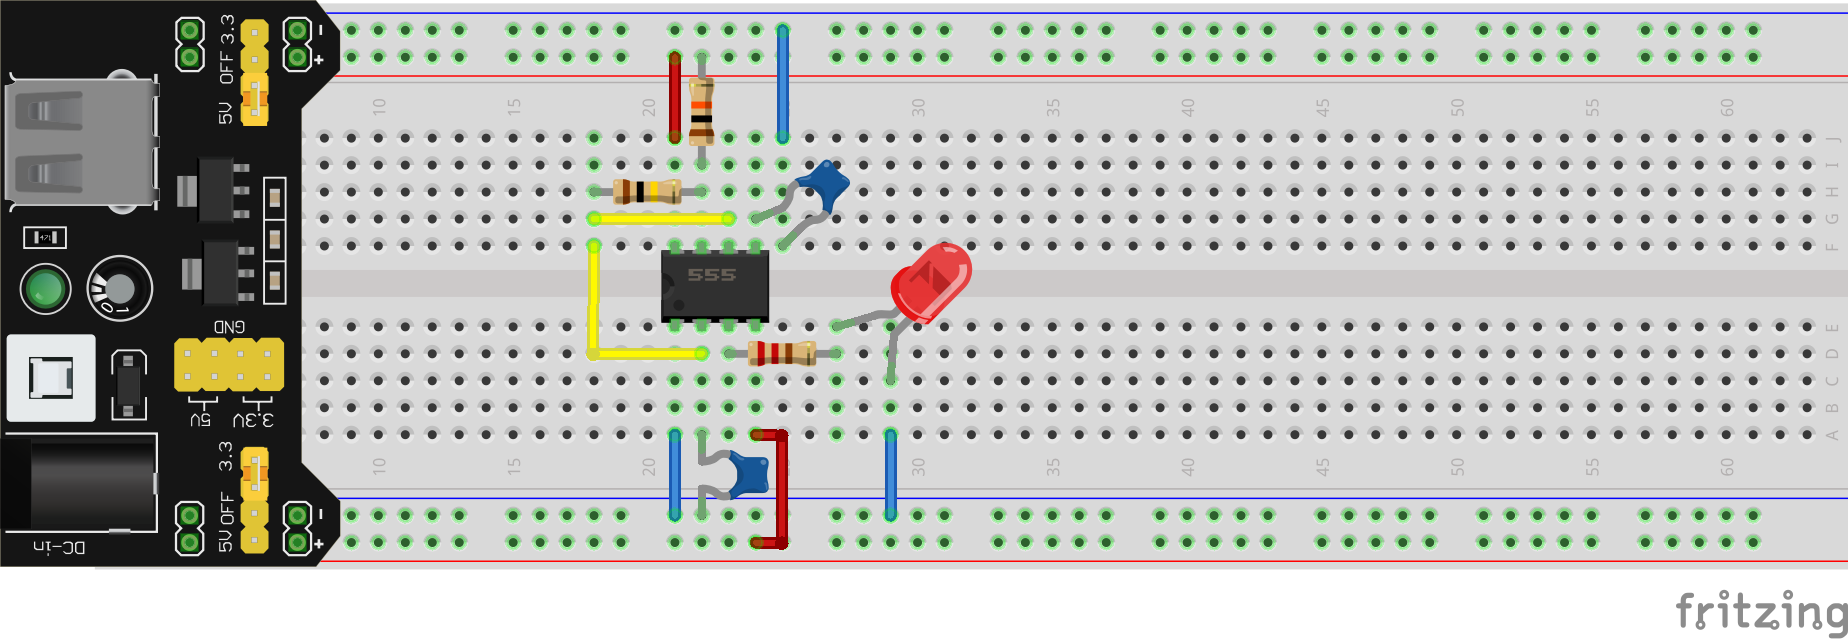
\includegraphics[width=0.8\textwidth]{lesson_circuits/L11/lesson_11.png}
    \caption{555 LED flasher Breadboard Schematic}
    \label{fig:555_led_sch}
\end{figure}
\begin{figure}[!htp]
    \centering
    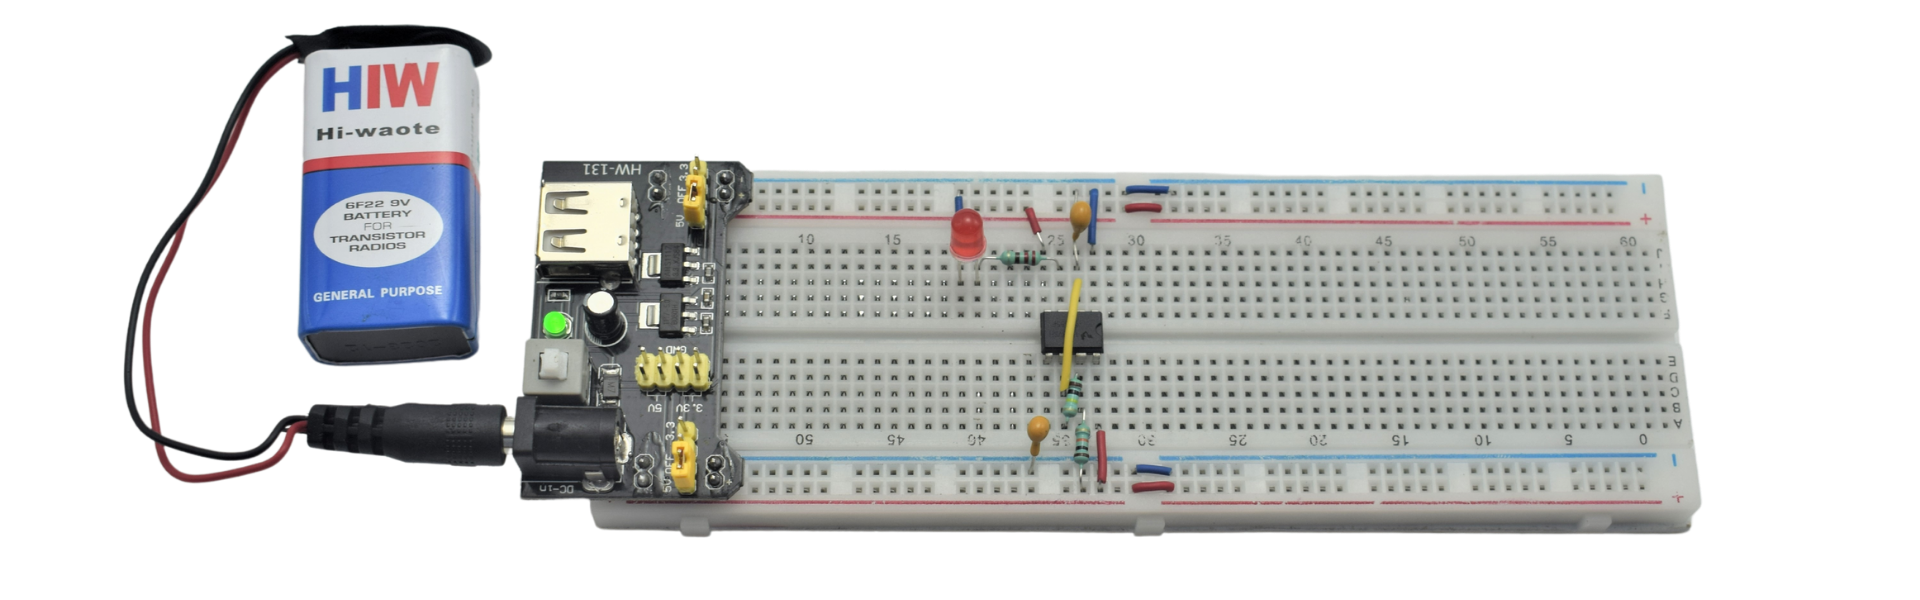
\includegraphics[width=\textwidth]{lesson_circuits/L11/L11-A.png}
    \caption{555 LED flasher: LED OFF}
    \label{fig:555_led_obb}
\end{figure}
\begin{figure}[!htp]
    \centering
    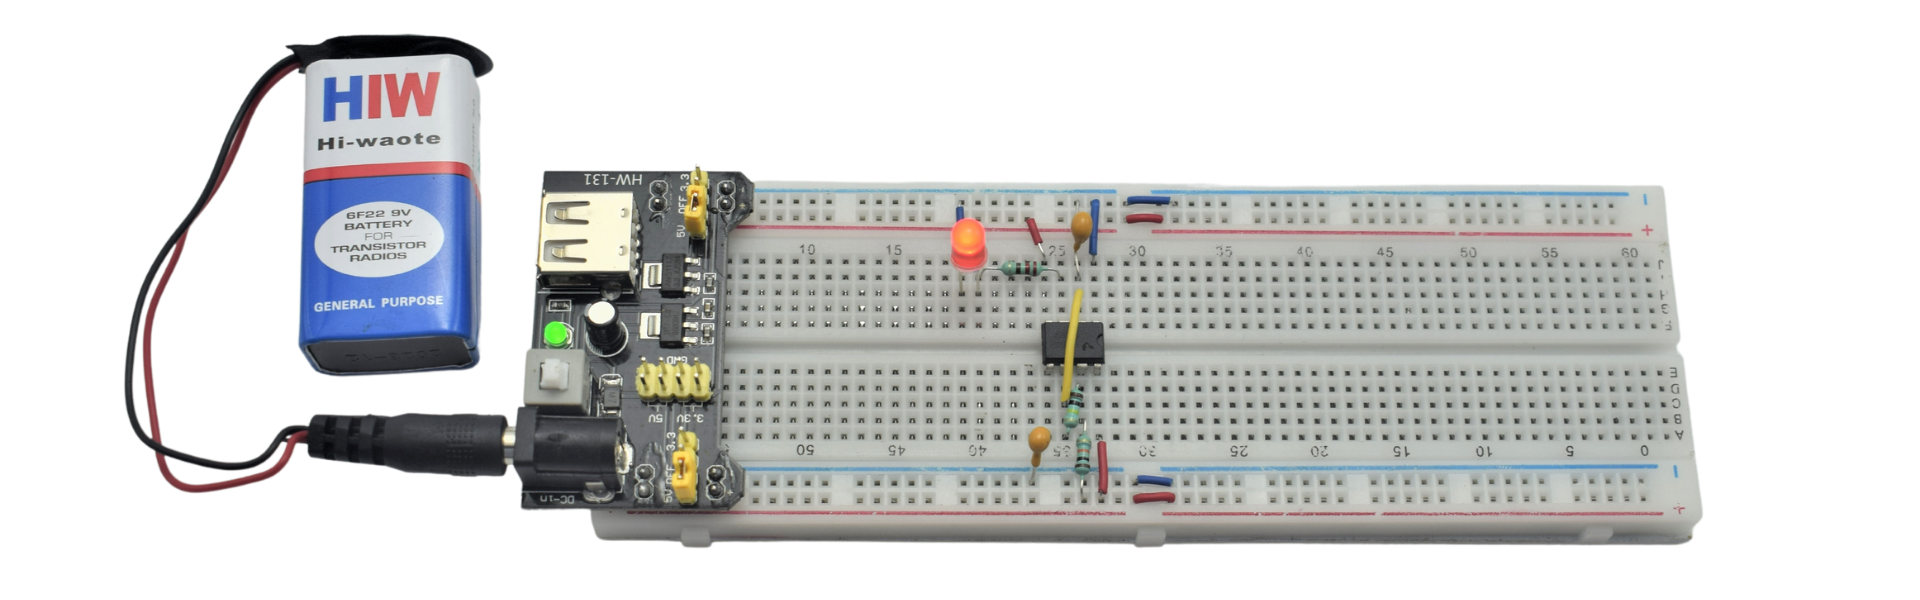
\includegraphics[width=\textwidth]{lesson_circuits/L11/L11-B.png}
    \caption{555 LED flasher: LED ON}
    \label{fig:555_led_obb1}
\end{figure}

\clearpage
\section{Lesson 12: 555 Dual LED Flasher}
\subsection{Objective}
In this activity we'll flash two LEDs on and off using astable 555 multivibrator circuit.
\subsection{Components Required}
\begin{enumerate}
    \item Breadboard Power Supply $\times$ 1
    \item 9V Battery $\times$ 1
    \item 9V Battery Connector $\times$ 1
    \item Breadboard $\times$ 1
    \item 555 IC $\times$ 1
    \item Red LED $\times$ 1
    \item Blue LED $\times$ 1
    \item \SI{220}{\ohm} $\times$ 2
    \item \SI{10}{\kilo\ohm} $\times$ 1
    \item \SI{100}{\kilo\ohm} $\times$ 1
    \item \SI{100}{\nano\farad} $\times$ 1
    \item \SI{10}{\micro\farad} $\times$ 1
    \item Male-Male jumper wire $\times$ 7
\end{enumerate}
\subsection{Circuit}
\begin{figure}[!htp]
    \centering
    \begin{circuitikz}[scale = 1.2]
        \TIMER555(0,0){1}
        \draw (1 GND) to[short, -*] ++(0,-0.7) node[ground](g1){};
        \draw (1 CTRL) to[C, l=$100\si{\nano\farad}$] ++(0,-0.5)
            to[short, -*] ++(0,-0.2)node[](ctr){} |- (g1);
        \draw (1 VCC) to[short, -*] ++(0,0.5) node[vcc](v1){$V_{cc}$};
        \draw (1 RESET) |- (v1);
        \draw (1 THR) to[short, -*] ++(-0.5,0) node[](s6){};
        \draw (1 TRG) to[short, -*] ++(-0.5,0) node[](s2){};
        \draw (1 DIS) to[short, -*] ++(-0.5,0) node[](s7){};
        \draw (s7) to[R, l_=$10\si{\kohm}$] ($(1 THR)-(0.5,0)$);
        \draw (s7) to[R, l=$100\si{\kohm}$] ++(0,1.5) |- (v1);
        \draw (s6) -- (s2) to[C, l_=$10\si{\micro\farad}$] ++(0,-1.5) |- (g1);
        \draw (1 OUT) to[short, -*] ++(0.5,0)node[](ll){} -- ++(0,-0.5) 
            to[R, l=$220\si{\ohm}$] ++ (0,-1)
            to[empty led, color=red] ++(0,-1.5) |- (ctr);
        \draw (ll) -- ++(0,0.5) 
            to[R, l=$220\si{\ohm}$] ++ (0,1)
            to[empty led, color=blue, invert, mirror] ++(0,1.5)
            to[short,-*] ++(-1.6,0);
    \end{circuitikz}
    \caption{555 Dual LED Flasher Circuit}
    \label{fig:555_dual_led_cir}
\end{figure}
\subsection{Circuit Explanation}
The circuit operates in astable mode as explained in section \ref{astablemode}. In this circuit one more LED is connected between 
the output pin and $V_{cc}$, in such a way that it glows up when output is low and turns off when output is high.
\subsection{Circuit Picture}
\begin{figure}[!htp]
    \centering
    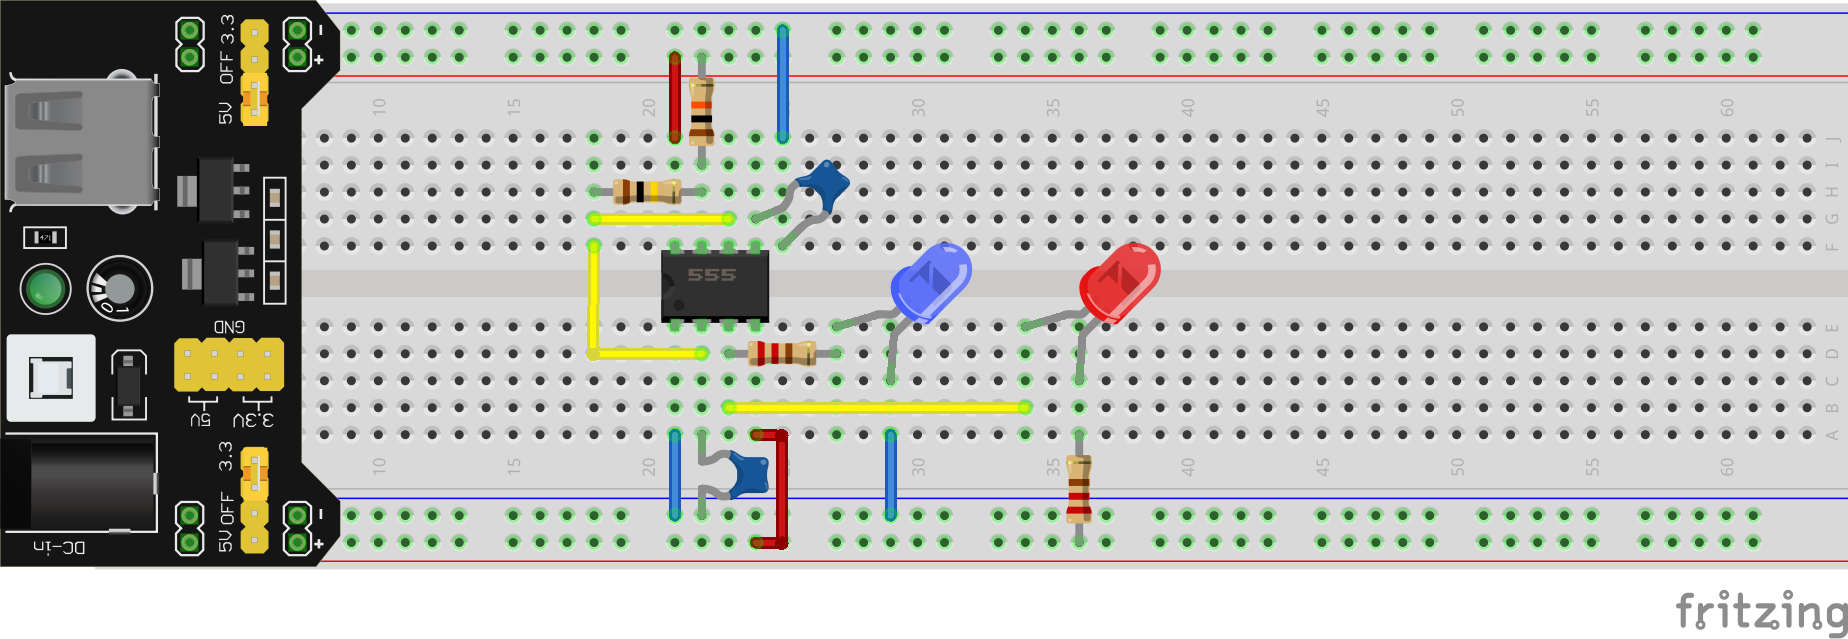
\includegraphics[width=0.8\textwidth]{lesson_circuits/L12/lesson_12.png}
    \caption{555 Dual LED flasher Breadboard Schematic}
    \label{fig:555_2led_sch}
\end{figure}
\begin{figure}[!htp]
    \centering
    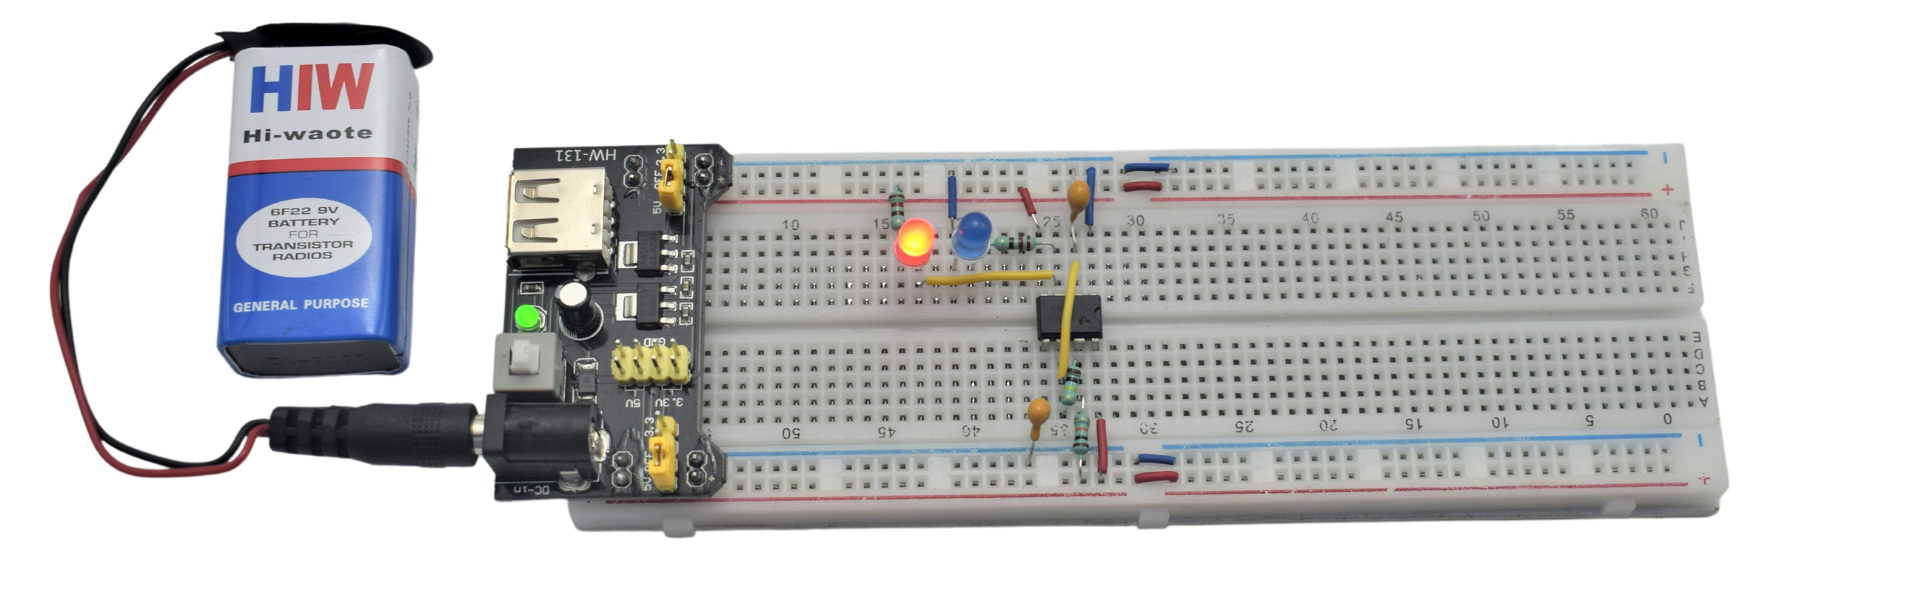
\includegraphics[width=\textwidth]{lesson_circuits/L12/L12-A.png}
    \caption{555 Dual LED flasher 1}
    \label{fig:555_2led_obb}
\end{figure}
\begin{figure}[!htp]
    \centering
    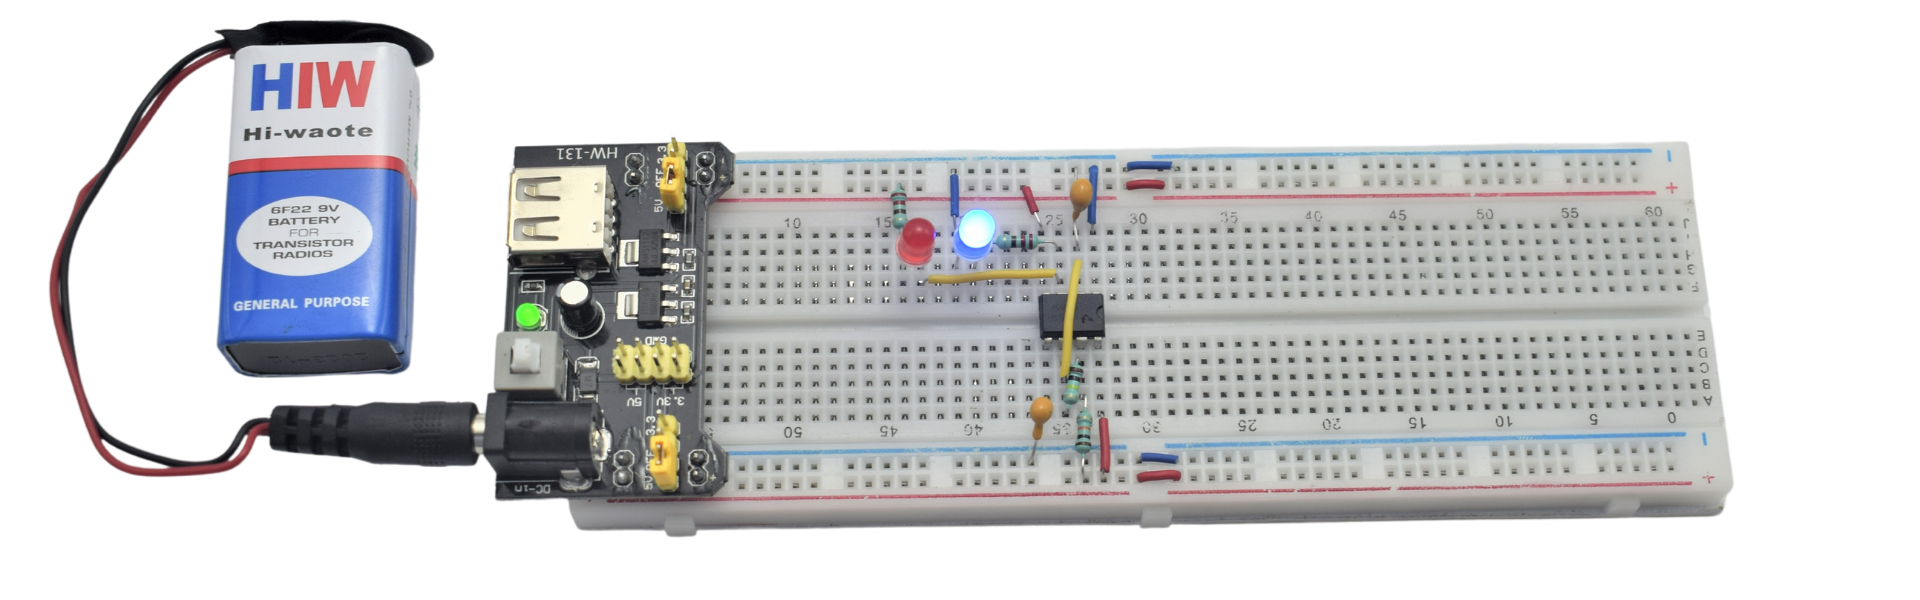
\includegraphics[width=\textwidth]{lesson_circuits/L12/L12-B.png}
    \caption{555 LED flasher 2}
    \label{fig:555_2led_obb1}
\end{figure}

\clearpage
\section{Lesson 13: Fading LED using 555}
\subsection{Objective}
In this activity we'll fade an LED up and down using astable 555 multivibrator circuit.
\subsection{Components Required}
\begin{enumerate}
    \item Breadboard Power Supply $\times$ 1
    \item 9V Battery $\times$ 1
    \item 9V Battery Connector $\times$ 1
    \item Breadboard $\times$ 1
    \item 555 IC $\times$ 1
    \item Red LED $\times$ 1
    \item 2N2222 $\times$ 1
    \item \SI{220}{\ohm} $\times$ 1
    \item \SI{10}{\kilo\ohm} $\times$ 1
    \item \SI{100}{\kilo\ohm} $\times$ 1
    \item \SI{1}{\Mohm} $\times$ 1
    \item \SI{100}{\nano\farad} $\times$ 1
    \item \SI{10}{\micro\farad} $\times$ 2
    \item Male-Male jumper wire $\times$ 11
\end{enumerate}
\subsection{Circuit}
\begin{figure}[!htp]
    \centering
    \begin{circuitikz}[scale = 1.2]
        \TIMER555(0,0){1}
        \draw (1 GND) to[short, -*] ++(0,-0.7) node[ground](g1){};
        \draw (1 CTRL) to[C, l=$100\si{\nano\farad}$] ++(0,-0.5)
            to[short, -*] ++(0,-0.2)node[](ctr){} |- (g1);
        \draw (1 VCC) to[short, -*] ++(0,0.5) node[vcc](v1){$V_{cc}$};
        \draw (1 RESET) to[short, -*] ++(0,0.5)node[](rst){} |- (v1);
        \draw (1 THR) to[short, -*] ++(-0.5,0) node[](s6){};
        \draw (1 TRG) to[short, -*] ++(-0.5,0) node[](s2){};
        \draw (1 DIS) to[short, -*] ++(-0.5,0) node[](s7){};
        \draw (s7) to[R, l_=$10\si{\kohm}$] ($(1 THR)-(0.5,0)$);
        \draw (s7) to[R, l=$100\si{\kohm}$] ++(0,1.5) |- (v1);
        \draw (s6) -- (s2) to[C, l_=$10\si{\micro\farad}$] 
            ++(0,-1.5) |- (g1);
        \draw ($(1 OUT) + (2,0)$) node[npn](t1){};
        \draw (1 OUT) to[R,l=$1\si{\Mohm}$] (t1.B);
        \draw (t1.B) to[short, *-] ++(0,-1)
                to[C, l_=$10\si{\uF}$] ++(0,-1.5)
                to[short, -*] ++(0,-0.7)node[](tt){} |- (ctr);
        \draw (t1.E) |- (tt);
        \draw (rst) to[R, l=$220\si{\ohm}$] ++(3.1,0)
                to[empty led, color=red] (t1.C);
    \end{circuitikz}
    \caption{Fading LED using 555}
    \label{fig:555_fade_led_cir}
\end{figure}
\subsection{Circuit Explanation}
In this circuit 555 operates in astable mode \ref{astablemode}. When the output is high, the capacitor connected to transistor base 
starts charging up, slowly lighting up the LED. And, as the output turns low, the capacitor slowly discharges through the transistor 
fading the LED off.
\subsection{Circuit Picture}
\begin{figure}[!htp]
    \centering
    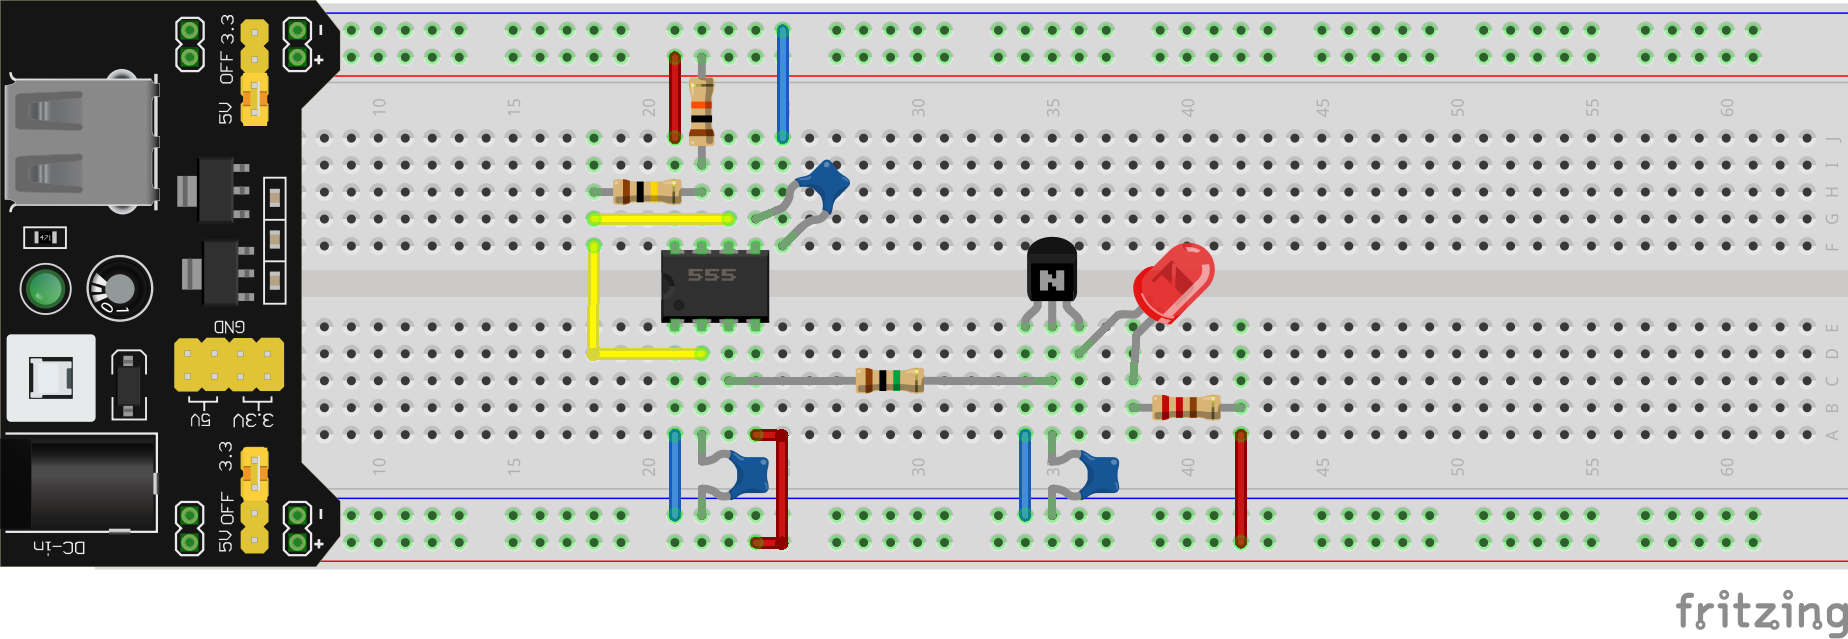
\includegraphics[width=0.8\textwidth]{lesson_circuits/L13/lesson_13.png}
    \caption{Fading LED using 555 Breadboard Schematic}
    \label{fig:555_fled_sch}
\end{figure}
\begin{figure}[!htp]
    \centering
    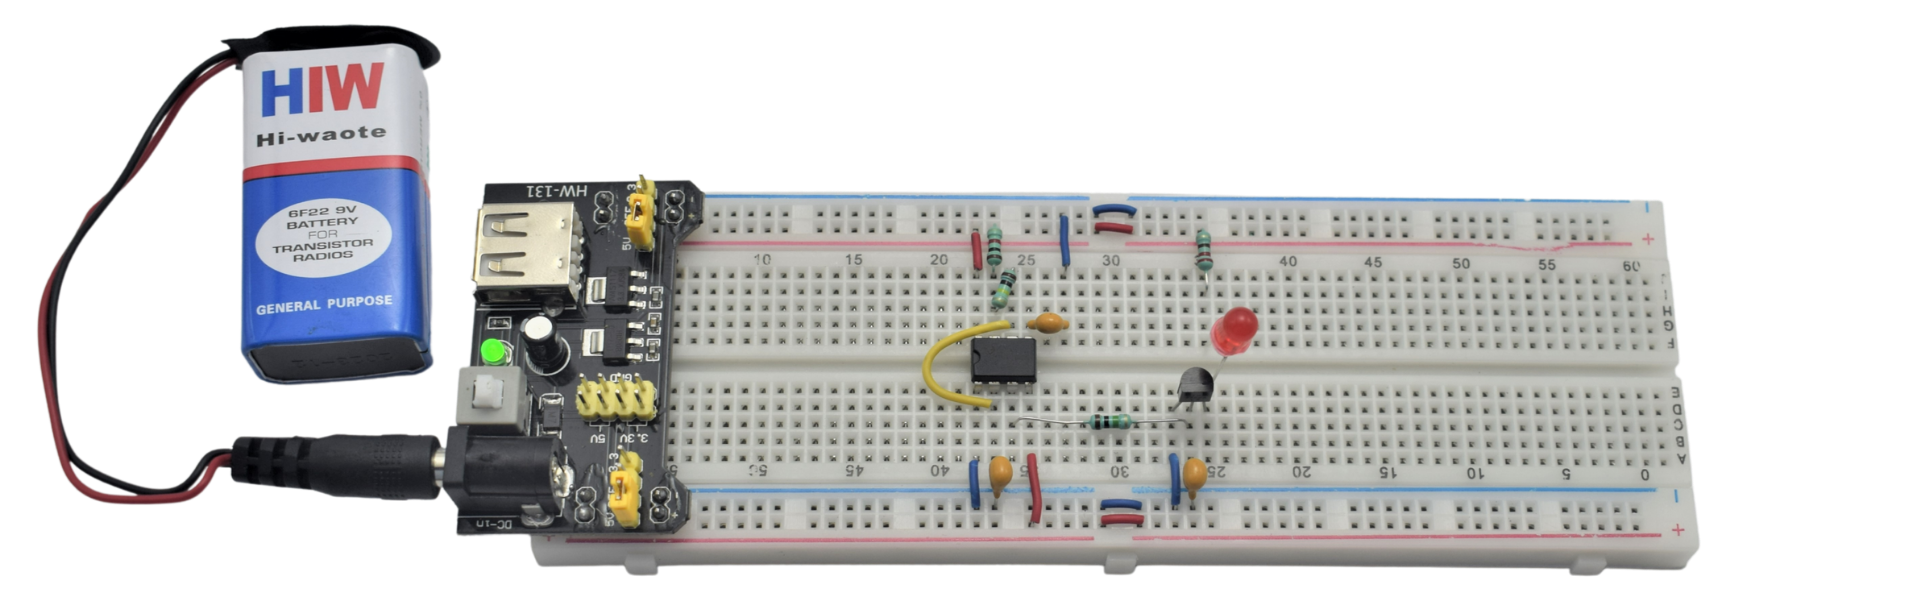
\includegraphics[width=\textwidth]{lesson_circuits/L13/L13-A.png}
    \caption{LED fading 1}
    \label{fig:555_fled_obb}
\end{figure}
\begin{figure}[!htp]
    \centering
    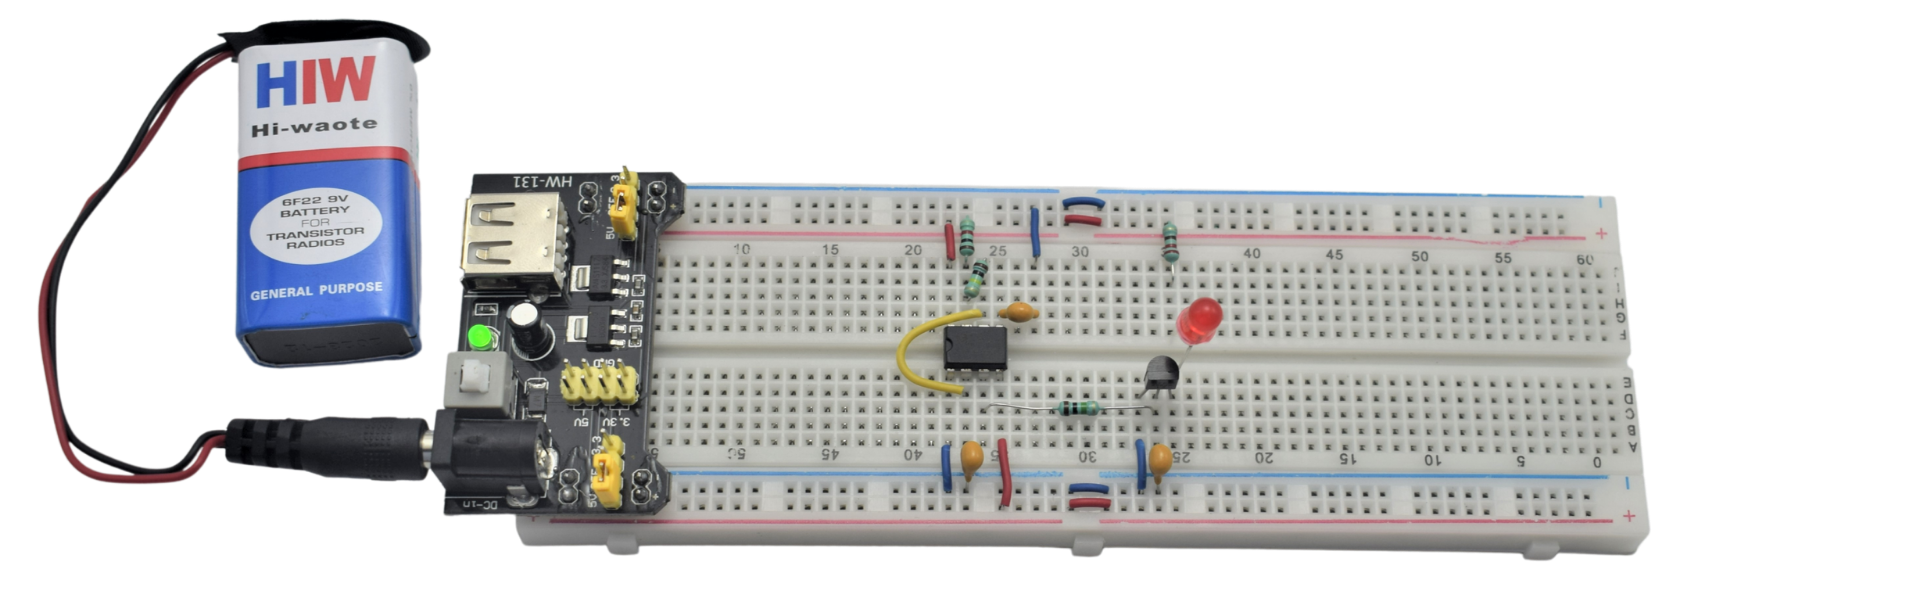
\includegraphics[width=\textwidth]{lesson_circuits/L13/L13-B.png}
    \caption{LED fading 2}
    \label{fig:555_fled_obb1}
\end{figure}

\clearpage
\section{Lesson 14: Bistable Button Flip/Flop using 555}
\subsection{Objective}
In this activity we'll create bistable 555 circuit.
\subsection{Components Required}
\begin{enumerate}
    \item Breadboard Power Supply $\times$ 1
    \item 9V Battery $\times$ 1
    \item 9V Battery Connector $\times$ 1
    \item Breadboard $\times$ 1
    \item 555 IC $\times$ 1
    \item Red LED $\times$ 1
    \item Push Button $\times$ 2
    \item \SI{220}{\ohm} $\times$ 1
    \item \SI{10}{\kilo\ohm} $\times$ 2
    \item \SI{100}{\nano\farad} $\times$ 2
    \item Male-Male jumper wire $\times$ 9
\end{enumerate}
\subsection{Circuit}
\begin{figure}[!htp]
    \centering
    \begin{circuitikz}[scale = 1.2]
        \TIMER555(0,0){1}
        \draw (1 GND) to[short, -*] ++(0,-0.7) node[ground](g1){};
        \draw (1 CTRL) to[C, l=$100\si{\nano\farad}$] ++(0,-0.5)
            to[short, -*] ++(0,-0.2)node[](ctr){} |- (g1);
        \draw (1 VCC) to[short, -*] ++(0,0.5) node[vcc](v1){$V_{cc}$};
        \draw (1 RESET) -- ++(0,0.2) -- ++(-3.5,0) -- ++(0,-3)
            to[short, -*] ++(-0.5,0)node[](br){} to[R,l=$10\si{\kohm}$] 
            ++(0,3.3)node[](j1){} |- (v1);
        \draw (1 TRG) to[short, -*] ++(-2,0)node[](bt){} 
            -- ++(0,1.2) to[R, l=$10\si{\kohm}$] ++(0,3.3) 
            to[short, -*] (j1);
        \draw (bt) to[push button, mirror, l_=TRIG] ++(0,-1.5) |- (g1);
        \draw (br) -- ++(0,-1.2) to[push button, l=RST] ++(0,-1.5) |- (g1);
        \draw (1 OUT) -- ++(0.5,0) -- ++(0,-0.5) 
            to[R, l=$220\si{\ohm}$] ++ (0,-1)
            to[empty led, color=red] ++(0,-1.5) |- (ctr);
    \end{circuitikz}
    \caption{Bistable Button Flip/Flop Circuit}
    \label{fig:555_bistable_cir}
\end{figure}
\subsection{Circuit Explanation}
This circuit is explained in section \ref{bistablemode}
\subsection{Circuit Picture}
\begin{figure}[!htp]
    \centering
    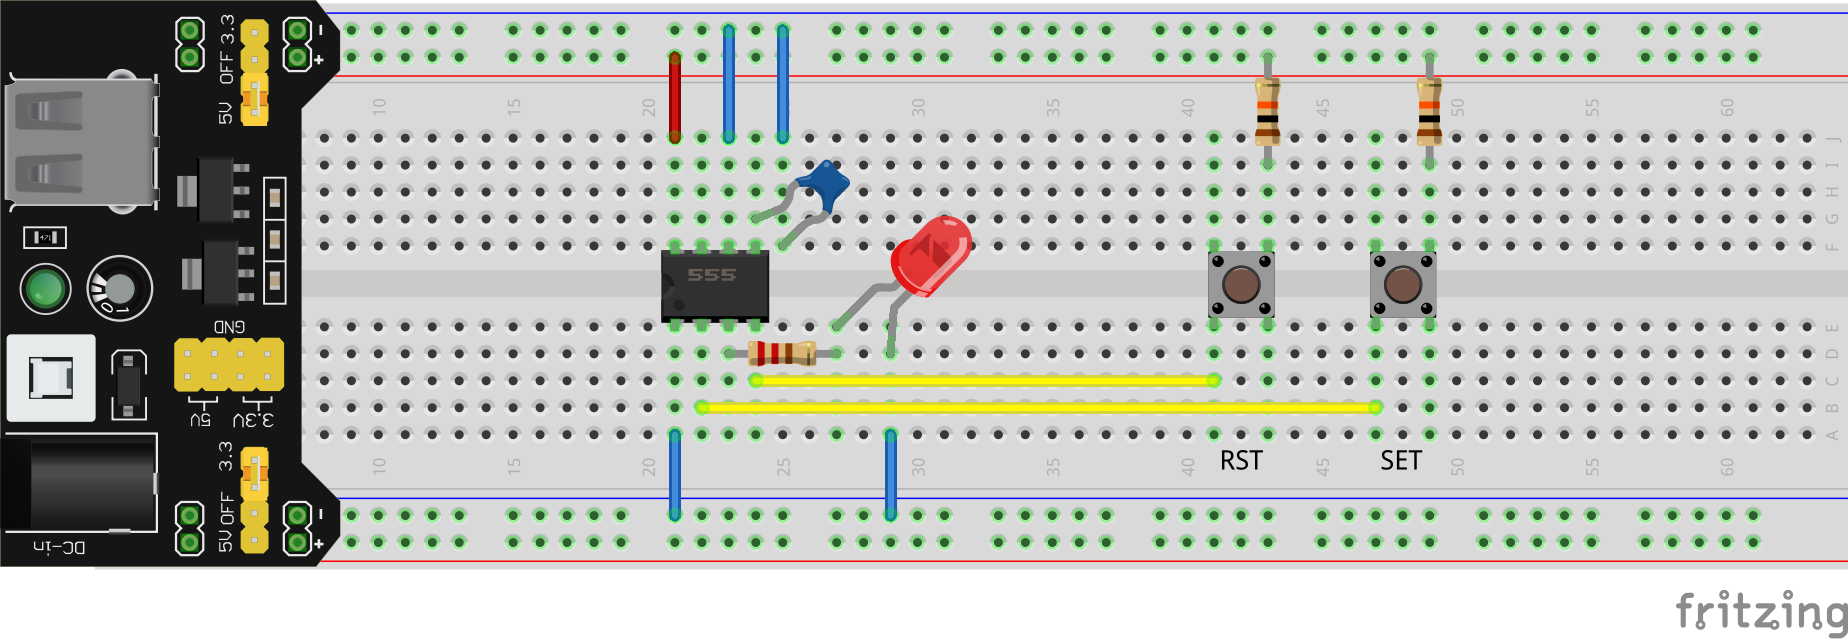
\includegraphics[width=0.8\textwidth]{lesson_circuits/L14/lesson_14.png}
    \caption{Bistable Button Flip/Flop using 555 Breadboard Schematic}
    \label{fig:555_ff_sch}
\end{figure}
\begin{figure}[!htp]
    \centering
    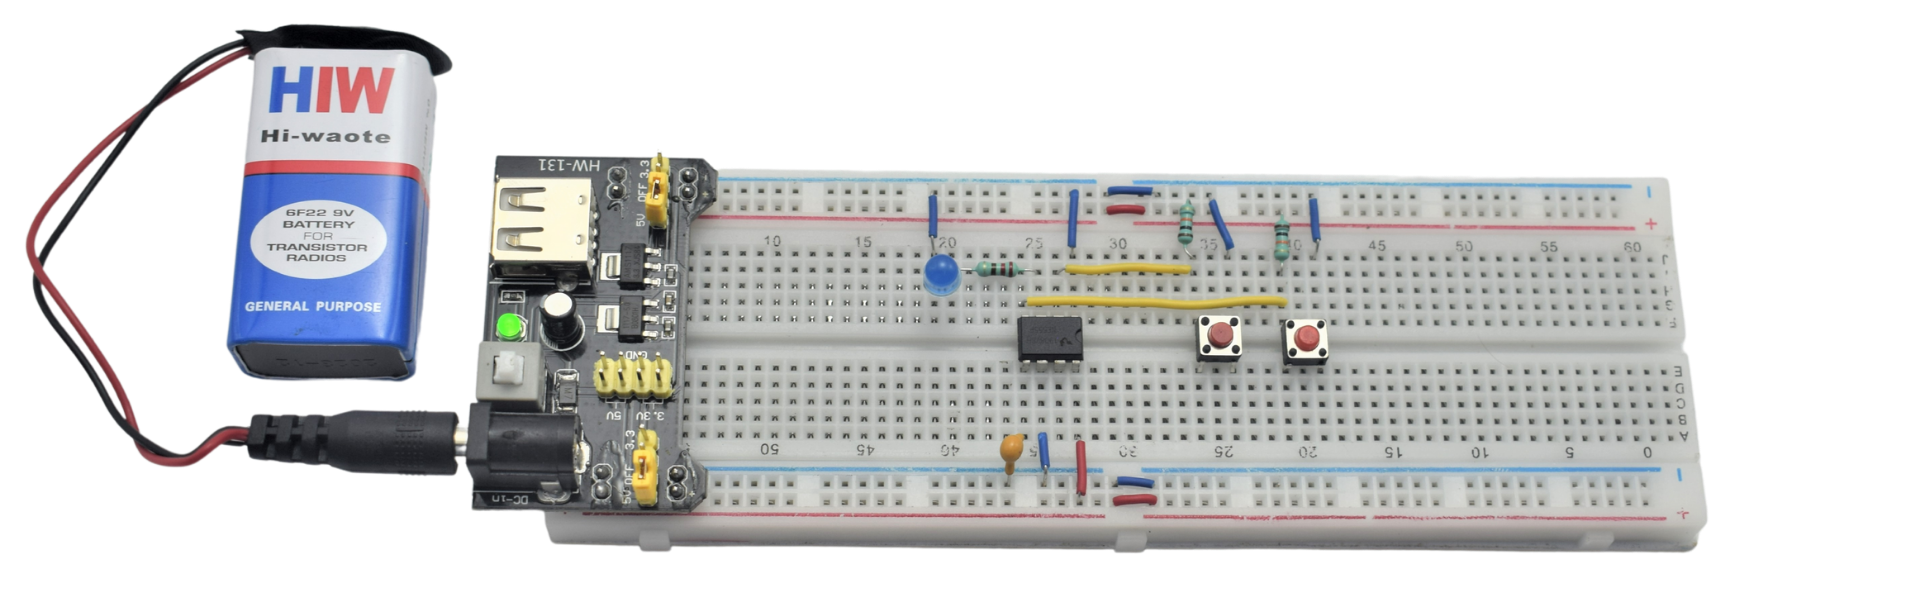
\includegraphics[width=\textwidth]{lesson_circuits/L14/L14-A.png}
    \caption{FF Idle}
    \label{fig:555_ff_obb}
\end{figure}
\begin{figure}[!htp]
    \centering
    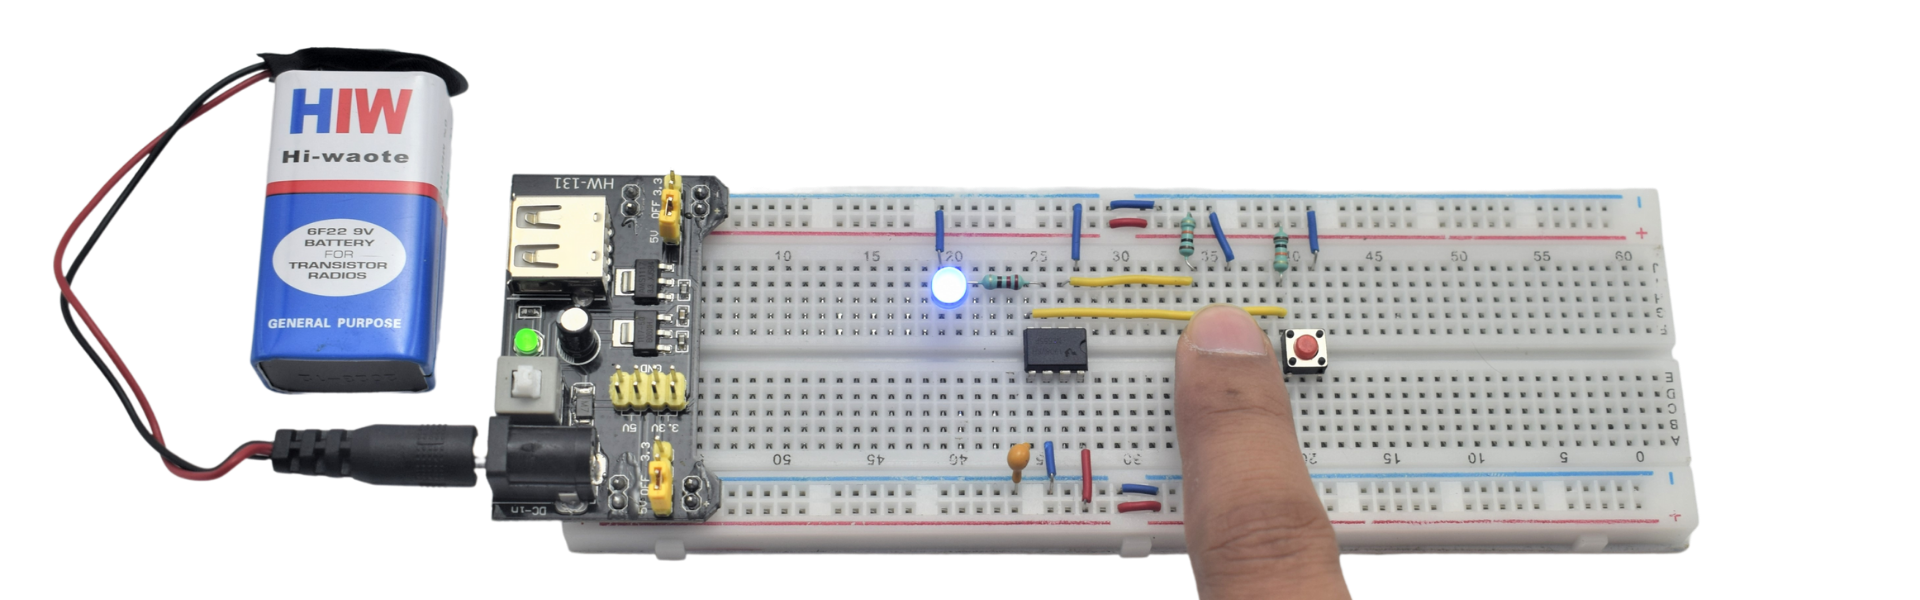
\includegraphics[width=\textwidth]{lesson_circuits/L14/L14-B.png}
    \caption{FF SET Button Pressed}
    \label{fig:555_ff_obb1}
\end{figure}
\begin{figure}[!htp]
    \centering
    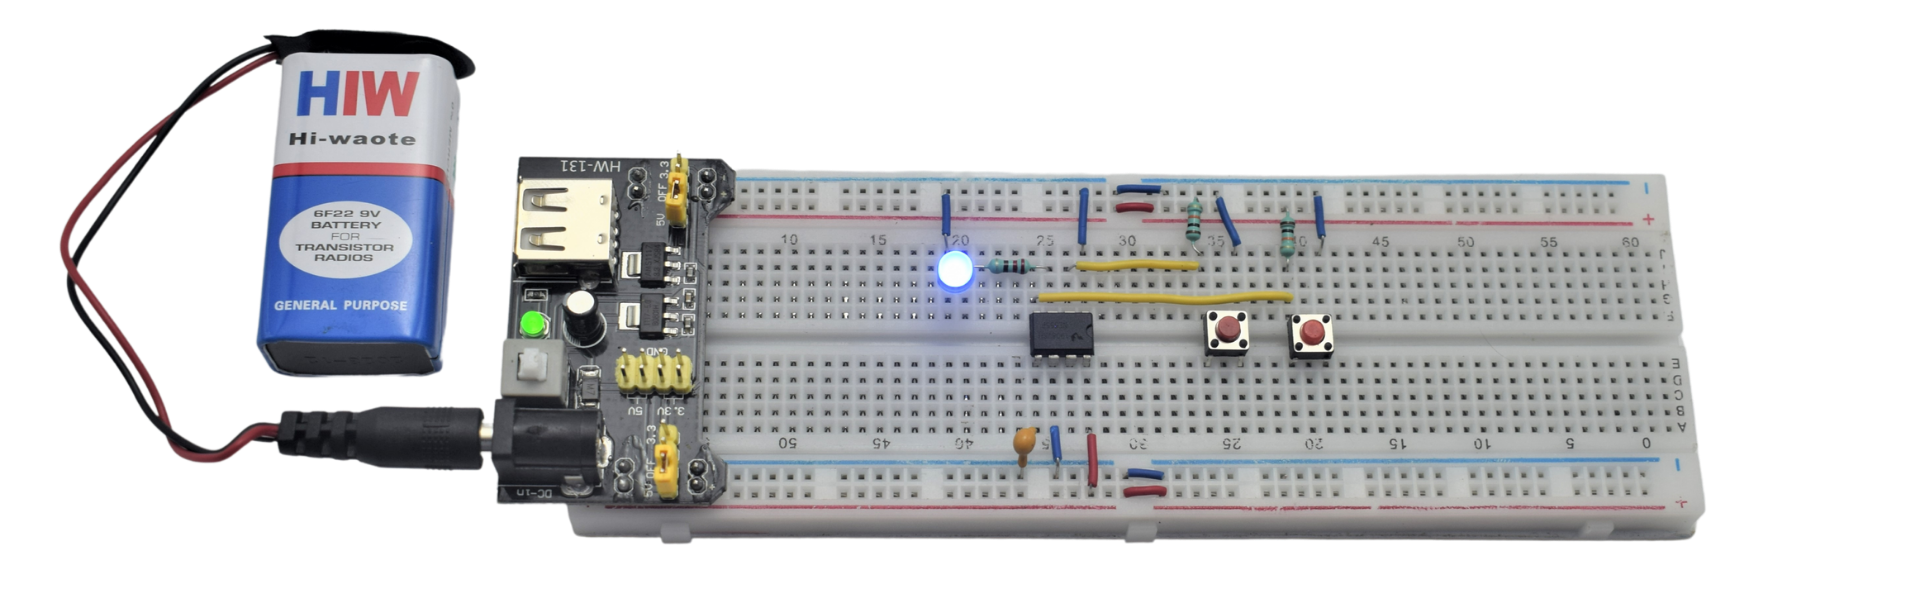
\includegraphics[width=\textwidth]{lesson_circuits/L14/L14-C.png}
    \caption{FF Idle after leaving SET button}
    \label{fig:555_ff_obb2}
\end{figure}
\begin{figure}[!htp]
    \centering
    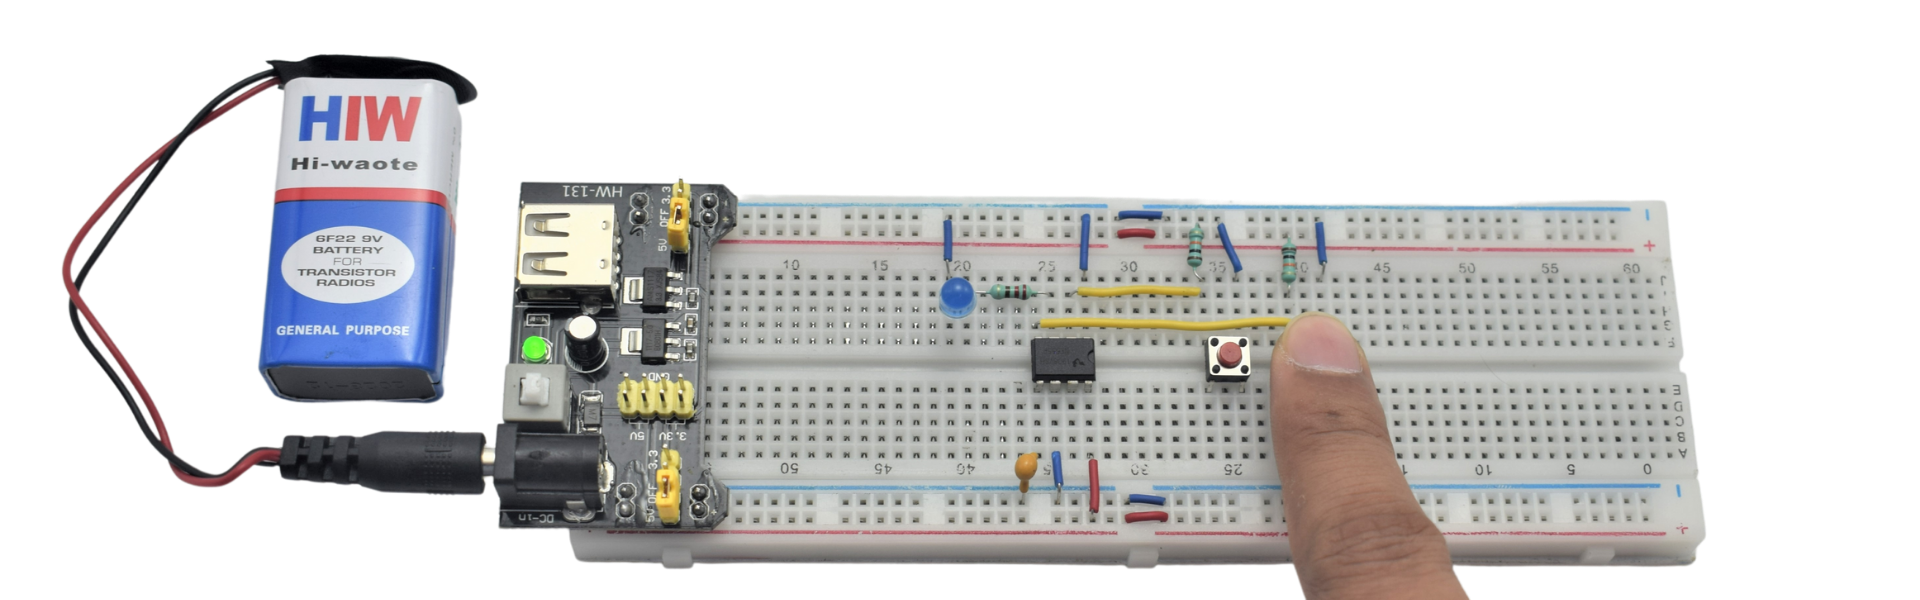
\includegraphics[width=\textwidth]{lesson_circuits/L14/L14-D.png}
    \caption{FF RST Button Pressed}
    \label{fig:555_ff_obb3}
\end{figure}
\begin{figure}[!htp]
    \centering
    \includegraphics[width=\textwidth]{lesson_circuits/L14/L14-E.png}
    \caption{FF Idle after leaving RST Button}
    \label{fig:555_ff_obb4}
\end{figure}
\clearpage
\section{Lesson 15: Toggle Switch with 555}
\subsection{Objective}
In this activity we'll create a toggle switch using bistable 555 circuit.
\subsection{Components Required}
\begin{enumerate}
    \item Breadboard Power Supply $\times$ 1
    \item 9V Battery $\times$ 1
    \item 9V Battery Connector $\times$ 1
    \item Breadboard $\times$ 1
    \item 555 IC $\times$ 1
    \item Red LED $\times$ 1
    \item Push Button $\times$ 1
    \item \SI{220}{\ohm} $\times$ 1
    \item \SI{10}{\kilo\ohm} $\times$ 2
    \item \SI{100}{\kilo\ohm} $\times$ 1
    \item \SI{100}{\nano\farad} $\times$ 2
    \item Male-Male jumper wire $\times$ 11
\end{enumerate}
\subsection{Circuit}
\begin{figure}[!htp]
    \centering
    \begin{circuitikz}[scale = 1.2]
        \TIMER555(0,0){1}
        \draw (1 GND) to[short, -*] ++(0,-0.7) node[ground](g1){};
        \draw (1 CTRL) to[C, l=$100\si{\nano\farad}$] ++(0,-0.5)
            to[short, -*] ++(0,-0.2)node[](ctr){} |- (g1);
        \draw (1 VCC) to[short, -*] ++(0,0.5) node[vcc](v1){$V_{cc}$};
        \draw (1 RESET) |- (v1);
        \draw (1 THR) to[short, -*] ++(-0.5,0) node[](s6){};
        \draw (1 TRG) to[short, -*] ++(-0.5,0) node[](s2){};
        \draw (s6) -- (s2);
        \draw (s6) to[R, l=$10\si{\kohm}$] ++(0,3) |- (v1);
        \draw (s2) to[R, l=$10\si{\kohm}$] ++(0,-1.7) |- (g1);
        \draw (1 OUT) -- ++(0.5,0)node[circ](oo){} -- ++(0,-0.5) 
            to[R, l=$220\si{\ohm}$] ++ (0,-1)
            to[empty led, color=red] ++(0,-1.7)node[circ](g2){} |- (ctr);
        \draw (oo) to[R, l=$100\si{\kohm}$] ++(1.5,0)node[circ](rc){}
            to[C, l=$100\si{\nF}$] ++(0,-2) |- (g2);
        \draw (rc) to[push button, mirror] ++(0,2.5) -- ++(-8,0) |- (s6);
    \end{circuitikz}
    \caption{Toggle Switch with 555 Circuit}
    \label{fig:555_toggle_cir}
\end{figure}
\subsection{Circuit Explanation}
In this circuit we control the voltage at pin 2 and 6 of the 555 IC with help of the push button and capacitor. When the circuit is 
powered on the capacitor $C_2$ is discharged, therefore it's upper plate is close to 0 volts. When the switch is pressed the voltage 
at pin 2 goes low, turning the output of 555 on. Now the LED is on and the capacitor starts charging.

Now, if we again press the switch, the capacitor is charged, therefore the upper plate is close to $V_{out}$ which makes the voltage 
at pin 6 high, turning the 555 output low. Now the capacitor discharges through the 555 output pin and LED is turned off.
\subsection{Circuit Picture}
\begin{figure}[!htp]
    \centering
    \includegraphics[width=0.8\textwidth]{lesson_circuits/L15/lesson_15.png}
    \caption{Toggle Switch using 555 Breadboard Schematic}
    \label{fig:555_ts_sch}
\end{figure}
\begin{figure}[!htp]
    \centering
    \includegraphics[width=\textwidth]{lesson_circuits/L15/L15-A.png}
    \caption{Idle}
    \label{fig:555_ts_obb}
\end{figure}
\begin{figure}[!htp]
    \centering
    \includegraphics[width=\textwidth]{lesson_circuits/L15/L15-B.png}
    \caption{Button Pressed: LED turned ON}
    \label{fig:555_ts_obb1}
\end{figure}
\begin{figure}[!htp]
    \centering
    \includegraphics[width=\textwidth]{lesson_circuits/L15/L15-C.png}
    \caption{Button released}
    \label{fig:555_ts_obb2}
\end{figure}
\begin{figure}[!htp]
    \centering
    \includegraphics[width=\textwidth]{lesson_circuits/L15/L15-D.png}
    \caption{Button Pressed: LED turned OFF}
    \label{fig:555_ts_obb3}
\end{figure}
\begin{figure}[!htp]
    \centering
    \includegraphics[width=\textwidth]{lesson_circuits/L15/L15-E.png}
    \caption{Button released}
    \label{fig:555_ts_obb4}
\end{figure}
\clearpage
\section{Lesson 16: Timer Delay using 555}
\subsection{Objective}
In this activity we'll use monostable 555 circuit to turn on an LED for fixed duration.
\subsection{Components Required}
\begin{enumerate}
    \item Breadboard Power Supply $\times$ 1
    \item 9V Battery $\times$ 1
    \item 9V Battery Connector $\times$ 1
    \item Breadboard $\times$ 1
    \item 555 IC $\times$ 1
    \item Red LED $\times$ 1
    \item Push Button $\times$ 1
    \item \SI{220}{\ohm} $\times$ 1
    \item \SI{10}{\kilo\ohm} $\times$ 1
    \item \SI{1}{\Mohm} $\times$ 1
    \item \SI{100}{\nano\farad} $\times$ 2
    \item \SI{100}{\nano\farad} $\times$ 2
    \item Male-Male jumper wire $\times$ 11
\end{enumerate}
\subsection{Circuit}
\begin{figure}[!htp]
    \centering
    \begin{circuitikz}[scale = 1.2]
        \TIMER555(0,0){1}
        \draw (1 GND) to[short, -*] ++(0,-0.7) node[ground](g1){};
        \draw (1 CTRL) to[C, l=$100\si{\nano\farad}$] ++(0,-0.5)
            to[short, -*] ++(0,-0.2)node[](ctr){} |- (g1);
        \draw (1 VCC) to[short, -*] ++(0,0.5) node[vcc](v1){$V_{cc}$};
        \draw (1 RESET) |- (v1);
        \draw (1 THR) to[short, -*] ++(-0.5,0) node[](s6){};
        \draw (1 TRG) to[short, -*] ++(-1.5,0) node[](s2){};
        \draw (1 DIS) to[short, -*] ++(-0.5,0) node[](s7){};
        \draw (s7) -- ($(1 THR)-(0.5,0)$);
        \draw (s7) to[R, l=$1\si{\Mohm}$] ++(0,1.5)node[circ](a){} |- (v1);
        \draw (s6) -- ++(0,-1) to[C, l_=$4.7\si{\uF}$] ++(0,-1.7)node[circ](b){} |- (g1);
        \draw (1 OUT) to[short, -*] ++(0.5,0)node[](ll){} -- ++(0,-0.5) 
            to[R, l=$220\si{\ohm}$] ++ (0,-1)
            to[empty led, color=red] ++(0,-1.5) |- (ctr);
        \draw (s2) to[R, l=$10\si{\kohm}$] ++(0,2) |- (a);
        \draw (s2) to[push button, mirror] ++(0,-1.7) |- (b);
    \end{circuitikz}
    \caption{Timer Delay using 555 Circuit}
    \label{fig:555_timer_cir}
\end{figure}
\subsection{Circuit Explanation}
This circuit is explained in section \ref{monostable}.
\subsection{Circuit Picture}
\begin{figure}[!htp]
    \centering
    \includegraphics[width=0.8\textwidth]{lesson_circuits/L15/lesson_15.png}
    \caption{Timer Delay using 555 Breadboard Schematic}
    \label{fig:555_timer_sch}
\end{figure}
\begin{figure}[!htp]
    \centering
    \includegraphics[width=\textwidth]{lesson_circuits/L15/L15-A.png}
    \caption{Idle}
    \label{fig:555_timer_obb}
\end{figure}
\begin{figure}[!htp]
    \centering
    \includegraphics[width=\textwidth]{lesson_circuits/L15/L15-B.png}
    \caption{Button Pressed}
    \label{fig:555_timer_obb1}
\end{figure}
\begin{figure}[!htp]
    \centering
    \includegraphics[width=\textwidth]{lesson_circuits/L15/L15-C.png}
    \caption{Button released}
    \label{fig:555_timer_obb2}
\end{figure}
\begin{figure}[!htp]
    \centering
    \includegraphics[width=\textwidth]{lesson_circuits/L15/L15-D.png}
    \caption{LED turned off after delay time}
    \label{fig:555_timer_obb3}
\end{figure}
\clearpage
\section{Lesson 17: Single Tone Buzzer with 555}
\subsection{Objective}
In this activity we'll use astable 555 circuit to produce sound using an buzzer.
\subsection{Components Required}
\begin{enumerate}
    \item Breadboard Power Supply $\times$ 1
    \item 9V Battery $\times$ 1
    \item 9V Battery Connector $\times$ 1
    \item Breadboard $\times$ 1
    \item 555 IC $\times$ 1
    \item Active Buzzer $\times$ 1
    \item \SI{10}{\kilo\ohm} $\times$ 1
    \item \SI{100}{\kilo\ohm} $\times$ 1
    \item \SI{100}{\nano\farad} $\times$ 1
    \item \SI{10}{\micro\farad} $\times$ 1
    \item Male-Male jumper wire $\times$ 7
\end{enumerate}
\subsection{Circuit}
\begin{figure}[!htp]
    \centering
    \begin{circuitikz}[scale = 1.2]
        \TIMER555(0,0){1}
        \draw (1 GND) to[short, -*] ++(0,-0.7) node[ground](g1){};
        \draw (1 CTRL) to[C, l=$100\si{\nano\farad}$] ++(0,-0.5)
            to[short, -*] ++(0,-0.2)node[](ctr){} |- (g1);
        \draw (1 VCC) to[short, -*] ++(0,0.5) node[vcc](v1){$V_{cc}$};
        \draw (1 RESET) |- (v1);
        \draw (1 THR) to[short, -*] ++(-0.5,0) node[](s6){};
        \draw (1 TRG) to[short, -*] ++(-0.5,0) node[](s2){};
        \draw (1 DIS) to[short, -*] ++(-0.5,0) node[](s7){};
        \draw (s7) to[R, l_=$10\si{\kohm}$] ($(1 THR)-(0.5,0)$);
        \draw (s7) to[R, l=$100\si{\kohm}$] ++(0,1.5) |- (v1);
        \draw (s6) -- (s2) to[C, l_=$10\si{\micro\farad}$] ++(0,-1.5) |- (g1);
        \draw (1 OUT) -- ++(0.5,0) -- ++(0,-0.5)
            to[loudspeaker, color=red] ++(0,-2.5) |- (ctr);
    \end{circuitikz}
    \caption{Single Tone Buzzer Circuit}
    \label{fig:555_sibuzz_cir}
\end{figure}
\subsection{Circuit Explanation}
In this circuit 555 is in astable mode, with a buzzer connected at the output.
\subsection{Circuit Picture}
\begin{figure}[!htp]
    \centering
    \includegraphics[width=0.8\textwidth]{lesson_circuits/L17/lesson_17.png}
    \caption{Single tone Buzzer with 555 Breadboard Schematic}
    \label{fig:555_sbuz_sch}
\end{figure}
\begin{figure}[!htp]
    \centering
    \includegraphics[width=\textwidth]{lesson_circuits/L17/L17-A.png}
    \caption{Single tone Buzzer}
    \label{fig:555_sbuz_obb}
\end{figure}
\clearpage
\section{Lesson 18: Short Beep}
\subsection{Objective}
In this activity we'll make a short beep sound.
\subsection{Components Required}
\begin{enumerate}
    \item Breadboard Power Supply $\times$ 1
    \item 9V Battery $\times$ 1
    \item 9V Battery Connector $\times$ 1
    \item Breadboard $\times$ 1
    \item 555 IC $\times$ 1
    \item Active Buzzer $\times$ 1
    \item 1N4007 Diode $\times$ 1
    \item \SI{10}{\kilo\ohm} $\times$ 1
    \item \SI{100}{\kilo\ohm} $\times$ 1
    \item \SI{1}{\Mohm} $\times$ 1
    \item \SI{100}{\nano\farad} $\times$ 1
    \item \SI{2.2}{\micro\farad} $\times$ 1
    \item Male-Male jumper wire $\times$ 10
\end{enumerate}
\subsection{Circuit}
\begin{figure}[!htp]
    \centering
    \begin{circuitikz}[scale = 1.2]
        \TIMER555(0,0){1}
        \draw (1 GND) to[short, -*] ++(0,-0.7) node[ground](g1){};
        \draw (1 CTRL) to[C, l=$100\si{\nano\farad}$] ++(0,-0.5)
            to[short, -*] ++(0,-0.2)node[](ctr){} |- (g1);
        \draw (1 VCC) to[short, -*] ++(0,0.5) node[vcc](v1){$V_{cc}$};
        \draw (1 RESET) |- (v1);
        \draw (1 THR) to[short, -*] ++(-0.5,0) node[](s6){};
        \draw (1 TRG) to[short, -*] ++(-0.5,0) node[](s2){};
        \draw (1 DIS) to[short, -*] ++(-0.5,0) node[](s7){};
        \draw (s7) to[R, l_=$1\si{\Mohm}$] ($(1 THR)-(0.5,0)$);
        \draw (s7) to[R, l=$10\si{\kohm}$] ++(0,1.5) |- (v1);
        \draw (s6) -- (s2) to[C, l_=$2.2\si{\micro\farad}$] ++(0,-1.5) |- (g1);
        \draw (1 OUT) -- ++(0.5,0) -- ++(0,-0.5)
            to[loudspeaker, color=red] ++(0,-2.5) |- (ctr);
        \draw (s7) -- ++(-1.5,0)
            to[R, l_=$100\si{\kohm}$] ++(0,-1.5)
            to[empty diode] ++(0,-1.5) |- (s2);
    \end{circuitikz}
    \caption{Short Beep Circuit}
    \label{fig:555_shbeep_cir}
\end{figure}
\subsection{Circuit Explanation}
In circuit is similar to the one explained in section \ref{astablemode}. In this circuit when the output is high, the capacitor 
get charged via the $100\si{\kohm}$ resistor and diode instead of $1\si{\Mohm}$, therefore it charges very rapidly.
\begin{figure}[!htp]
    \centering
    \begin{circuitikz}[scale = 1.2]
        \TIMER555(0,0){1}
        \draw (1 GND) to[short, -*] ++(0,-0.7) node[ground](g1){};
        \draw (1 CTRL) to[C, l=$100\si{\nano\farad}$] ++(0,-0.5)
            to[short, -*] ++(0,-0.2)node[](ctr){} |- (g1);
        \draw (1 VCC) to[short, -*] ++(0,0.5) node[vcc](v1){$V_{cc}$};
        \draw (1 RESET) |- (v1);
        \draw (1 THR) to[short, -*] ++(-0.5,0) node[](s6){};
        \draw (1 TRG) to[short, -*] ++(-0.5,0) node[](s2){};
        \draw (1 DIS) to[short, -*] ++(-0.5,0) node[](s7){};
        \draw (s7) to[R, l_=$1\si{\Mohm}$] ($(1 THR)-(0.5,0)$);
        \draw (s7) to[R, l=$10\si{\kohm}$] ++(0,1.5) |- (v1);
        \draw (s6) -- (s2) to[C, l_=$2.2\si{\micro\farad}$] ++(0,-1.5) |- (g1);
        \draw (1 OUT) -- ++(0.5,0) -- ++(0,-0.5)
            to[loudspeaker, color=red] ++(0,-2.5) |- (ctr);
        \draw (s7) -- ++(-1.5,0)
            to[R, l_=$100\si{\kohm}$] ++(0,-1.5)
            to[empty diode] ++(0,-1.5) |- (s2);
        \draw[->, red]
            ($(v1)+(-0.2,0.2)$) -- ++(-2,0) -- ++(0,-2) -- ++(-1.4,0)
            -- ++(0,-2.5) -- ++(0.6,0) -- ++(0,-0.4);
    \end{circuitikz}
    \caption{Short Beep Circuit : Capacitor Charging}
    \label{fig:555_shbeep_charge_cir}
\end{figure}

And when the output is low, it discharges through $1\si{\Mohm}$ resistor. Since the high time is very less compared to the 
low time, the buzzer produces a short beep tone.
\begin{figure}[!htp]
    \centering
    \begin{circuitikz}[scale = 1.2]
        \TIMER555(0,0){1}
        \draw (1 GND) to[short, -*] ++(0,-0.7) node[ground](g1){};
        \draw (1 CTRL) to[C, l=$100\si{\nano\farad}$] ++(0,-0.5)
            to[short, -*] ++(0,-0.2)node[](ctr){} |- (g1);
        \draw (1 VCC) to[short, -*] ++(0,0.5) node[vcc](v1){$V_{cc}$};
        \draw (1 RESET) |- (v1);
        \draw (1 THR) to[short, -*] ++(-0.5,0) node[](s6){};
        \draw (1 TRG) to[short, -*] ++(-0.5,0) node[](s2){};
        \draw (1 DIS) to[short, -*] ++(-0.5,0) node[](s7){};
        \draw (s7) to[R, l_=$1\si{\Mohm}$] ($(1 THR)-(0.5,0)$);
        \draw (s7) to[R, l=$10\si{\kohm}$] ++(0,1.5) |- (v1);
        \draw (s6) -- (s2) to[C, l_=$2.2\si{\micro\farad}$] ++(0,-1.5) |- (g1);
        \draw (1 OUT) -- ++(0.5,0) -- ++(0,-0.5)
            to[loudspeaker, color=red] ++(0,-2.5) |- (ctr);
        \draw (s7) -- ++(-1.5,0)
            to[R, l_=$100\si{\kohm}$] ++(0,-1.5)
            to[empty diode] ++(0,-1.5) |- (s2);
        \draw[<-, blue]
            ($(1 DIS)-(0.2,0.2)$) -- ++(-0.5,0) -- ++(0,-3.2);
    \end{circuitikz}
    \caption{Short Beep Circuit : Capacitor Discharging}
    \label{fig:555_shbeep_discharge_cir}
\end{figure}

\subsection{Circuit Picture}
\begin{figure}[!htp]
    \centering
    \includegraphics[width=0.8\textwidth]{lesson_circuits/L18/lesson_18.png}
    \caption{Short Beep using 555 Breadboard Schematic}
    \label{fig:555_sbeep_sch}
\end{figure}
\begin{figure}[!htp]
    \centering
    \includegraphics[width=\textwidth]{lesson_circuits/L18/L18-A.png}
    \caption{Short Beep}
    \label{fig:555_sbeep_obb}
\end{figure}
\clearpage
\section{Lesson 19: Break Beam Detector using 555 and LDR}
\subsection{Objective}
In this activity we'll make a break beam detector circuit.
\subsection{Components Required}
\begin{enumerate}
    \item Breadboard Power Supply $\times$ 1
    \item 9V Battery $\times$ 1
    \item 9V Battery Connector $\times$ 1
    \item Breadboard $\times$ 1
    \item 555 IC $\times$ 1
    \item Passive Buzzer $\times$ 1
    \item White LED $\times$ 1
    \item LDR $\times$ 1
    \item \SI{220}{\ohm} $\times$ 1
    \item \SI{10}{\kilo\ohm} $\times$ 3
    \item \SI{100}{\nano\farad} $\times$ 2
    \item \SI{10}{\micro\farad} $\times$ 1
    \item Male-Male jumper wire $\times$ 15
\end{enumerate}
\subsection{Circuit}
\begin{figure}[!htp]
    \centering
    \begin{circuitikz}[scale = 1.2]
        \TIMER555(0,0){1}
        \draw (0,-3.5) node[npn](t1){T1};
        \draw (1 GND) -- (t1.C);
        \draw (t1.E) -- ++(0,-0.2) node[circ](g1){} -- node[ground](g1){} ++(0,0);
        \draw (1 CTRL) to[C, l=$100\si{\nano\farad}$] ++(0,-0.5)
            to[short, -*] ++(0,-0.2)node[](ctr){} |- (g1);
        \draw (1 VCC) to[short, -*] ++(0,0.5) node[vcc](v1){$V_{cc}$};
        \draw (1 RESET) |- (v1);
        \draw (1 THR) to[short, -*] ++(-0.5,0) node[](s6){};
        \draw (1 TRG) to[short, -*] ++(-0.5,0) node[](s2){};
        \draw (1 DIS) to[short, -*] ++(-0.5,0) node[](s7){};
        \draw (s7) to[R, l_=$10\si{\kohm}$] ($(1 THR)-(0.5,0)$);
        \draw (s7) to[R, l=$100\si{\kohm}$] ++(0,1.5)node[circ](sh1){} |- (v1);
        \draw (s6) -- (s2) to[C, l_=$10\si{\micro\farad}$] ++(0,-1.5) |- (g1);
        \draw (1 OUT) -- ++(0.5,0) -- ++(0,-0.5) 
            to[C, l=$10\si{\uF}$] ++ (0,-1)
            to[loudspeaker] ++(0,-1.5) |- (ctr);
        \draw (-4,0) node[npn](t2){T2};
        \draw (t1.B) -| (t2.E);
        \draw (t2.C) -- ++(0,2.35)node[circ](t2c){} |- (sh1);
        \draw (t2.B) -- ++(-1,0)node[circ](t2b){};
        \draw (t2c) -- ++(-1.7,0)node[circ](ab){} to[R, l=$10\si{\kohm}$] (t2b)
            to[sR] ++(0,-4.35)node[circ](g3){} to[short,-*] ++(3.2,0);
        \draw (ab) -- ++(-1,0) to[R, l_=$220\si{\ohm}$] ++(0,-3) to[empty led] ++(0,-4) |- (g3);
    \end{circuitikz}
    \caption{Break Beam Detector Circuit}
    \label{fig:555_bbdet_cir}
\end{figure}
\subsection{Circuit Explanation}
When there is no barrier in between the LED and LDR, the resistance of LDR is very low and there the base transistor $T2$ is near 
ground potential or 0 volt and is in cut-off mode. Since, $T2$ is off, $T1$ is also off and the 555 will not work, because the GND 
pin is connected to collector of $T1$.

When there is obstruction between light and LDR, the resistance of LDR goes high, turning the $T2$ on, which turns on the $T1$. 
Now $T1$ is and 555 will start operating in astable mode.
\subsection{Circuit Picture}
\begin{figure}[!htp]
    \centering
    \includegraphics[width=0.8\textwidth]{lesson_circuits/L19/lesson_19.png}
    \caption{Break Beam Detector using 555 and LDR Breadboard Schematic}
    \label{fig:555_bbdet_sch}
\end{figure}
\begin{figure}[!htp]
    \centering
    \includegraphics[width=\textwidth]{lesson_circuits/L19/L19-A.png}
    \caption{No Obstacle: Buzzer OFF}
    \label{fig:555_bbdet_obb}
\end{figure}
\begin{figure}[!htp]
    \centering
    \includegraphics[width=\textwidth]{lesson_circuits/L19/L19-B.png}
    \caption{Obstacle: Buzzer ON}
    \label{fig:555_bbdet_obb1}
\end{figure}
\clearpage
\section{Lesson 20: Light reactive buzzer using 555 and LDR}
\subsection{Objective}
In this activity we'll make a light reactive tone generator.
\subsection{Components Required}
\begin{enumerate}
    \item Breadboard Power Supply $\times$ 1
    \item 9V Battery $\times$ 1
    \item 9V Battery Connector $\times$ 1
    \item Breadboard $\times$ 1
    \item 555 IC $\times$ 1
    \item Passive Buzzer $\times$ 1
    \item LDR $\times$ 1
    \item \SI{10}{\kilo\ohm} $\times$ 1
    \item \SI{100}{\nano\farad} $\times$ 2
    \item \SI{10}{\micro\farad} $\times$ 1
    \item Male-Male jumper wire $\times$ 9
\end{enumerate}
\subsection{Circuit}
\begin{figure}[!htp]
    \centering
    \begin{circuitikz}[scale = 1.2]
        \TIMER555(0,0){1}
        \draw (1 GND) to[short, -*] ++(0,-0.7) node[ground](g1){};
        \draw (1 CTRL) to[C, l=$100\si{\nano\farad}$] ++(0,-0.5)
            to[short, -*] ++(0,-0.2)node[](ctr){} |- (g1);
        \draw (1 VCC) to[short, -*] ++(0,0.5) node[vcc](v1){$V_{cc}$};
        \draw (1 RESET) |- (v1);
        \draw (1 THR) to[short, -*] ++(-0.5,0) node[](s6){};
        \draw (1 TRG) to[short, -*] ++(-0.5,0) node[](s2){};
        \draw (1 DIS) to[short, -*] ++(-0.5,0) node[](s7){};
        \draw (s7) to[sR] ($(1 THR)-(0.5,0)$);
        \draw (s7) to[R, l=$100\si{\kohm}$] ++(0,1.5) |- (v1);
        \draw (s6) -- (s2) to[C, l_=$10\si{\micro\farad}$] ++(0,-1.5) |- (g1);
        \draw (1 OUT) -- ++(0.5,0) -- ++(0,-0.5) 
            to[C, l=$10\si{\uF}$] ++ (0,-1)
            to[loudspeaker] ++(0,-1.5) |- (ctr);
    \end{circuitikz}
    \caption{Light Reactive Buzzer Circuit}
    \label{fig:555_lrbuzz_cir}
\end{figure}
\subsection{Circuit Explanation}
In this circuit the 555 is in astable mode, but the $R_2$ resistor is replaced with an LDR, so according to the change in intensity 
of light falling on the LDR, the frequency of output is changed, changing the tone generated by the buzzer.
\subsection{Circuit Picture}
\begin{figure}[!htp]
    \centering
    \includegraphics[width=0.8\textwidth]{lesson_circuits/L20/lesson_20.png}
    \caption{Light reactive Buzzer Breadboard Schematic}
    \label{fig:555_ldrbuzz_sch}
\end{figure}
\begin{figure}[!htp]
    \centering
    \includegraphics[width=\textwidth]{lesson_circuits/L20/L20-A.png}
    \caption{Light reactive Buzzer}
    \label{fig:555_ldrbuzz_obb}
\end{figure}
\clearpage
\section{Lesson 21: Audio Tone/Siren}
\subsection{Objective}
In this activity we'll make an audio tone/siren generator.
\subsection{Components Required}
\begin{enumerate}
    \item Breadboard Power Supply $\times$ 1
    \item 9V Battery $\times$ 1
    \item 9V Battery Connector $\times$ 1
    \item Breadboard $\times$ 1
    \item 555 IC $\times$ 2
    \item Passive Buzzer $\times$ 1
    \item \SI{10}{\kilo\ohm} $\times$ 5
    \item \SI{100}{\kilo\ohm} $\times$ 1
    \item \SI{100}{\nano\farad} $\times$ 2
    \item \SI{10}{\micro\farad} $\times$ 2
    \item Male-Male jumper wire $\times$ 14
\end{enumerate}
\subsection{Circuit}
\begin{figure}[!htp]
    \centering
    \begin{circuitikz}[scale = 1]
        \TIMER555(0,0){1}
        \draw (1 GND) to[short, -*] ++(0,-0.7) node[ground](g1){};
        \draw (1 CTRL) to[C, l=$100\si{\nano\farad}$] ++(0,-0.5)
            to[short, -*] ++(0,-0.2)node[](ctr){} |- (g1);
        \draw (1 VCC) to[short, -*] ++(0,0.5) node[vcc](v1){$V_{cc}$};
        \draw (1 RESET) |- (v1);
        \draw (1 THR) to[short, -*] ++(-0.5,0) node[](s6){};
        \draw (1 TRG) to[short, -*] ++(-0.5,0) node[](s2){};
        \draw (1 DIS) to[short, -*] ++(-0.5,0) node[](s7){};
        \draw (s7) to[R, l_=$10\si{\kohm}$] ($(1 THR)-(0.5,0)$);
        \draw (s7) to[R, l=$100\si{\kohm}$] ++(0,1.5) |- (v1);
        \draw (s6) -- (s2) to[C, l_=$10\si{\micro\farad}$] ++(0,-1.5) |- (g1);
        
        \TIMER555(8,0){2};
        \draw (2 GND) to[short, -*] ++(0,-0.7) node[ground](g21){};
        \draw (2 VCC) to[short, -*] ++(0,0.5) node[vcc](v21){$V_{cc}$};
        \draw (2 RESET) |- (v21);
        \draw (2 THR) to[short, -*] ++(-0.5,0) node[](s26){};
        \draw (2 TRG) to[short, -*] ++(-0.5,0) node[](s22){};
        \draw (2 DIS) to[short, -*] ++(-0.5,0) node[](s27){};
        \draw (s27) to[R, l=$10\si{\kohm}$] ($(2 THR)-(0.5,0)$);
        \draw (s27) to[R, l=$100\si{\kohm}$] ++(0,1.5) |- (v21);
        \draw (s26) -- (s22) to[C, l_=$10\si{\micro\farad}$] ++(0,-1.5) |- (g21);
        \draw (2 OUT) -- ++(0.5,0) -- ++(0,-0.5) 
            to[C, l=$10\si{\uF}$] ++ (0,-1)
            to[loudspeaker] ++(0,-1.5) |- (g21);
        \draw (2 CTRL) -- ++(0,-0.2) -- ++(-5.5,0) 
            to[R, l=$10\si{\kohm}$] ++(0,2) |- (1 OUT);
    \end{circuitikz}
    \caption{Audio Tone/Siren Circuit}
    \label{fig:555_ausiren_cir}
\end{figure}
\subsection{Circuit Explanation}
In this circuit both the 555 are running in astable. But, we are controlling the input voltage of the second 555 using the output 
of the first, such that whenever the output of first 555 changes, the frequency of output of second 555 changes, producing two 
different tone after each interval. 
\subsection{Circuit Picture}
\begin{figure}[!htp]
    \centering
    \includegraphics[width=0.8\textwidth]{lesson_circuits/L21/lesson_21.png}
    \caption{Audio Tone/Siren Breadboard Schematic}
    \label{fig:555_audsi_sch}
\end{figure}
\begin{figure}[!htp]
    \centering
    \includegraphics[width=\textwidth]{lesson_circuits/L21/L21-A.png}
    \caption{Audio Tone/Siren}
    \label{fig:555_audsi_obb}
\end{figure}
\clearpage
\section{Lesson 22: Traffic Light}
\subsection{Objective}
In this activity we'll make a Traffic Light using 555.
\subsection{Components Required}
\begin{enumerate}
    \item Breadboard Power Supply $\times$ 1
    \item 9V Battery $\times$ 1
    \item 9V Battery Connector $\times$ 1
    \item Breadboard $\times$ 1
    \item 555 IC $\times$ 2
    \item Red LED $\times$ 1
    \item Yellow LED $\times$ 1
    \item Green LED $\times$ 1
    \item 2N2222 $\times$ 1
    \item \SI{220}{\ohm} $\times$ 3
    \item \SI{330}{\ohm} $\times$ 3
    \item \SI{10}{\kilo\ohm} $\times$ 2
    \item \SI{1}{\Mohm} $\times$ 2
    \item \SI{100}{\nano\farad} $\times$ 2
    \item \SI{2.2}{\micro\farad} $\times$ 1
    \item \SI{10}{\micro\farad} $\times$ 2
    \item Male-Male jumper wire $\times$ 22
\end{enumerate}
\subsection{Circuit}
\begin{figure}[!htp]
    \centering
    \begin{circuitikz}[scale = 1]
        \TIMER555(0,0){1}
        \draw (1 GND) to[short, -*] ++(0,-0.7) node[ground](g1){};
        \draw (1 CTRL) to[C, l=$100\si{\nano\farad}$] ++(0,-0.5)
            to[short, -*] ++(0,-0.2)node[](ctr){} |- (g1);
        \draw (1 VCC) to[short, -*] ++(0,0.5) node[vcc](v1){$V_{cc}$};
        \draw (1 RESET) |- (v1);
        \draw (1 THR) to[short, -*] ++(-0.5,0) node[](s6){};
        \draw (1 TRG) to[short, -*] ++(-0.5,0) node[](s2){};
        \draw (1 DIS) to[short, -*] ++(-0.5,0) node[](s7){};
        \draw (s7) to[R, l_=$10\si{\kohm}$] ($(1 THR)-(0.5,0)$);
        \draw (s7) to[R, l=$100\si{\kohm}$] ++(0,1.5) |- (v1);
        \draw (s6) -- (s2) to[C, l_=$10\si{\micro\farad}$] ++(0,-1.5) |- (g1);
        \draw (1 OUT) to[short, -*] ++(0.5,0)node[](ll1){};
        \draw (ll1) -- ++(0,0.5) 
            to[R, l=$220\si{\ohm}$] ++ (0,1)
            to[empty led, color=red, invert, mirror] ++(0,1.5)
            to[short,-*] ++(-1.6,0)node[](vr1){};
        \TIMER555(8,0){2};
        \draw (2 GND) to[short, -*] ++(0,-0.7) node[ground](g21){};
        \draw (2 CTRL) to[C, l=$100\si{\nano\farad}$] ++(0,-0.5)
            to[short, -*] ++(0,-0.2)node[](ctr2){} |- (g21);
        %\draw (2 VCC) to[short, -*] ++(0,0.5) node[vcc](v21){$V_{cc}$};
        \draw (2 RESET) to[short, -*] ++(0,0.8) node[vcc](v21){$V_{cc}$};
        \draw (2 THR) to[short, -*] ++(-0.5,0) node[](s26){};
        \draw (2 TRG) to[short, -*] ++(-0.5,0) node[](s22){};
        \draw (2 DIS) to[short, -*] ++(-0.5,0) node[](s27){};
        \draw (s27) to[R, l_=$10\si{\kohm}$] ($(2 THR)-(0.5,0)$);
        \draw (s27) to[R, l=$100\si{\kohm}$] ++(0,1.5) |- (v21);
        \draw (s26) -- (s22) to[C, l_=$10\si{\micro\farad}$] ++(0,-1.5) |- (g21);
        \draw (2 OUT) to[short, -*] ++(0.5,0)node[](ll){} -- ++(0,-0.5) 
            to[R, l=$220\si{\ohm}$] ++ (0,-1)
            to[empty led, color=green] ++(0,-1.5) |- (ctr2);
        \draw (ll) -- ++(0,0.5) 
            to[R, l=$220\si{\ohm}$] ++ (0,1)
            to[empty led, color=yellow, invert, mirror] ++(0,1.5)
            to[short, -*] ($(2 VCC)+(0,0.5)$);
        
        \draw (ll1) -- ++(1.5,0) to[R, l=$330\si{\ohm}$] ++(0,3)node[](bb){};
        \draw (bb) node[npn, anchor=B, rotate=90](t1){T1};
        \draw (vr1) |- (t1.C);
        \draw (t1.E) -| (2 VCC);
    \end{circuitikz}
    \caption{Traffic Light Circuit}
    \label{fig:555_traffic_cir}
\end{figure}
\subsection{Circuit Explanation}
In this circuit both the 555 are in astable mode, and the supply of the second 555 is controlled by the output of first. To better 
understand what's going on look at the figure \ref{fig:555_traffic_time_cir}.
\begin{figure}[!htp]
    \centering
    \begin{circuitikz}[scale = 1.2]
        \draw (0,0) -- (1.5,0) -- (1.5,1) -- (5,1) -- (5,0) -- (6,0);
        \draw (0,-2) -- (1.5,-2) -- (1.5,-1) -- (4,-1) -- (4,-2) -- (6,-2);
        \draw (0.75, 0.5) node[]{$R_{ON}$};
        \draw (3.25, 0.5) node[]{$R_{OFF}$};
        \draw (2.75, -1.5) node[]{$G_{ON}$};
        \draw (4.5, -1.5) node[]{$Y_{ON}$};
    \end{circuitikz}
    \caption{Traffic Light Timing Diagram}
    \label{fig:555_traffic_time_cir}
\end{figure}

When the output of first 555 is low, the second 555 is off. Red light is on and both yellow and green are off. As soon as the output 
of the first 555 goes high, the second 555 starts working turning the green light on and both red and yellow are off. The on and off 
time of 555 output are set such that before the red light turns on again, the yellow light is momentarily turned on.
\subsection{Circuit Picture}
\begin{figure}[!htp]
    \centering
    \includegraphics[width=0.8\textwidth]{lesson_circuits/L22/lesson_22.png}
    \caption{Traffic Light Breadboard Schematic}
    \label{fig:555_trlight_sch}
\end{figure}
\begin{figure}[!htp]
    \centering
    \includegraphics[width=\textwidth]{lesson_circuits/L22/L22-A.png}
    \caption{Green Light On}
    \label{fig:555_trlight_obb}
\end{figure}
\begin{figure}[!htp]
    \centering
    \includegraphics[width=\textwidth]{lesson_circuits/L22/L22-C.png}
    \caption{Yellow Light On}
    \label{fig:555_trlight_obb1}
\end{figure}
\begin{figure}[!htp]
    \centering
    \includegraphics[width=\textwidth]{lesson_circuits/L22/L22-B.png}
    \caption{Red Light On}
    \label{fig:555_trlight_obb2}
\end{figure}
\clearpage
\section{Lesson 23: Doorbell}
\subsection{Objective}
In this activity we'll make a doorbell system using 555.
\subsection{Components Required}
\begin{enumerate}
    \item Breadboard Power Supply $\times$ 1
    \item 9V Battery $\times$ 1
    \item 9V Battery Connector $\times$ 1
    \item Breadboard $\times$ 1
    \item 555 IC $\times$ 2
    \item 2N2222 $\times$ 3
    \item Passive Buzzer $\times$ 1
    \item Push Button $\times$ 1
    \item \SI{1}{\kilo\ohm} $\times$ 3
    \item \SI{10}{\kilo\ohm} $\times$ 3
    \item \SI{1}{\Mohm} $\times$ 1
    \item \SI{100}{\nano\farad} $\times$ 2
    \item \SI{1}{\micro\farad} $\times$ 1
    \item Male-Male jumper wire $\times$ 23
\end{enumerate}
\subsection{Circuit}
\begin{figure}[!htp]
    \centering
    \begin{circuitikz}[scale = 1]
        \TIMER555(0,0){1}
        \draw (1 GND) to[short, -*] ++(0,-1.7) node[ground](g1){};
        \draw (1 CTRL) to[C, l=$100\si{\nano\farad}$] ++(0,-0.5)
            to[short, -*] ++(0,-1.2)node[](ctr){} |- (g1);
        \draw (1 VCC) to[short, -*] ++(0,0.5) node[vcc](v1){$V_{cc}$};
        \draw (1 RESET) |- (v1);
        \draw (1 THR) to[short, -*] ++(-0.5,0) node[](s6){};
        \draw (1 TRG) to[short, -*] ++(-1.5,0) node[](s2){};
        \draw (1 DIS) to[short, -*] ++(-0.5,0) node[](s7){};
        \draw (s7) -- ($(1 THR)-(0.5,0)$);
        \draw (s7) to[R, l=$1\si{\Mohm}$] ++(0,1.5)node[circ](a){} |- (v1);
        \draw (s6) -- ++(0,-1) to[C, l_=$1\si{\uF}$] ++(0,-2.7)node[circ](b){} |- (g1);
        \draw (s2) to[R, l=$10\si{\kohm}$] ++(0,2) |- (a);
        \draw (s2) node[npn,anchor=C](t2){$T2$};
        
        \TIMER555(8,0){2}
        %\draw (2 GND) to[short, -*] ++(0,-1.7) node[ground](2g1){};
        \draw (2 VCC) to[short, -*] ++(0,0.5) node[vcc](2v1){$V_{cc}$};
        \draw (2 RESET) to[short, -*] ++(0,0.5)node[](r2){} |- (2v1);
        \draw (2 THR) to[short, -*] ++(-0.5,0) node[](2s6){};
        \draw (2 TRG) to[short, -*] ++(-0.5,0) node[](2s2){};
        \draw (2 DIS) to[short, -*] ++(-0.5,0) node[](2s7){};
        \draw (2s7) to[R, l_=$10\si{\kohm}$] ($(2 THR)-(0.5,0)$);
        \draw (2s7) to[R, l=$10\si{\kohm}$] ++(0,1.5) |- (2v1);
        \draw (2s6) -- (2s2) to[C, l_=$100\si{\nF}$] ++(0,-1.5) 
            to[short, -*] ++(0,-1.2) node[ground](2g1){};
        \draw (2 OUT) -- ++(0.5,0) -- ++(0,-0.5)
            to[loudspeaker] ++(0,-1.5) |- (2g1);
        \draw (2 GND) -- ++(0,-0.17)node[](1ct){};
        \draw (2 CTRL) -- ++(0,-0.17)node[](1ct2){};
        \draw (1ct) node[npn, anchor=C](t1){$T1$};
        \draw (1ct2) node[npn, anchor=E,rotate=180](t3){};
        \draw (t1.E) node[circ]{};
        
        \draw (1 OUT) -| ++(1.2,-0.5) 
            to[R, l=$220\si{\ohm}$] ++ (0,-2)
            |- (t1.B);
        \draw (t2.E) |- (b);
        \draw (t2.B) -- ++(-0.5,0) to[R, l=$1\si{\kohm}$] ++(0,2.5)node[circ](c){}
            to[push button] ++(0,2) -- ++(0,0.77) to[short, -*] ++(1.35,0);
        \draw (c) -- ++(-1,0) -- ++(0,-5.5) -| (t3.B);
        \draw (t3.C) |- ++(2.5,-0.3) |- (r2);
    \end{circuitikz}
    \caption{Doorbell Circuit}
    \label{fig:555_doorbell_cir}
\end{figure}
\subsection{Circuit Explanation}
In this circuit the first 555 is in monostable mode and the second one is in astable mode. When powered on, the second 555 is 
off, as it's ground is disconnected. When the button is pressed the output of first 555 goes high, turning on the second one. 
And, the output of first 555 also controls the internal voltage of the second 555, so when the button is pressed the second 555 
sounds the buzzer in one frequency and when the button is released it sound the buzzer in different frequency till the output of 
the first 555 goes low.
\subsection{Circuit Picture}
\begin{figure}[!htp]
    \centering
    \includegraphics[width=0.8\textwidth]{lesson_circuits/L23/lesson_23.png}
    \caption{Doorbell Breadboard Schematic}
    \label{fig:555_doorbell_sch}
\end{figure}
\begin{figure}[!htp]
    \centering
    \includegraphics[width=\textwidth]{lesson_circuits/L23/L23-A.png}
    \caption{Idle: Buzzer OFF}
    \label{fig:555_doorbell_obb}
\end{figure}
\begin{figure}[!htp]
    \centering
    \includegraphics[width=\textwidth]{lesson_circuits/L23/L23-B.png}
    \caption{Button Pressed: Buzzer ON for sometime}
    \label{fig:555_doorbell_obb1}
\end{figure}
\clearpage
\section{Lesson 24: PWM Speed Controller}
\subsection{Objective}
In this activity we'll control a dc motor using 555 as PWM generator.
\subsection{Components Required}
\begin{enumerate}
    \item Breadboard Power Supply $\times$ 1
    \item 9V Battery $\times$ 1
    \item 9V Battery Connector $\times$ 1
    \item Breadboard $\times$ 1
    \item 555 IC $\times$ 1
    \item 2N2222 $\times$ 1
    \item DC Motor $\times$ 1
    \item Propeller $\times$ 1
    \item 1N4007 Diode $\times$ 2
    \item \SI{1}{\kilo\ohm} $\times$ 1
    \item \SI{2}{\kilo\ohm} $\times$ 1
    \item \SI{10}{\kilo\ohm} $\times$ 1
    \item \SI{10}{\kilo\ohm} Potentiometer $\times$ 1
    \item \SI{100}{\nano\farad} $\times$ 2
    \item \SI{10}{\micro\farad} $\times$ 1
    \item Male-Male jumper wire $\times$ 11
\end{enumerate}
\subsection{Circuit}
\begin{figure}[!htp]
    \centering
    \begin{circuitikz}[scale = 1.2]
        \TIMER555(0,0){1}
        \draw (1 GND) to[short, -*] ++(0,-0.7) node[ground](g1){};
        \draw (1 CTRL) to[C, l=$100\si{\nano\farad}$] ++(0,-0.5)
            to[short, -*] ++(0,-0.2)node[](ctr){} |- (g1);
        \draw (1 VCC) to[short, -*] ++(0,0.5) node[vcc](v1){$V_{cc}$};
        \draw (1 RESET) to[short, -*] ++(0,0.5)node[](rst){} |- (v1);
        \draw (1 THR) to[short, -*] ++(-0.5,0) node[](s6){};
        \draw (1 TRG) to[short, -*] ++(-0.5,0) node[](s2){};
        \draw (1 DIS) to[short, -*] ++(-0.5,0) node[](s7){};
        \draw (s7) to[R, l=$100\si{\kohm}$] ++(0,1.5) |- (v1);
        \draw (s6) -- (s2) to[C, l_=$10\si{\micro\farad}$] 
            ++(0,-1.5) |- (g1);
        \draw ($(1 OUT) + (2,0)$) node[npn](t1){};
        \draw (1 OUT) to[R,l=$2\si{\kohm}$] (t1.B);
        \draw (t1.E) |- (ctr);
        \draw (rst) -- ++(3.1,0)node[circ](rr){}
                to[sV, color=white, name=M1] (t1.C);
        \mymotor{M1}{90}
        \draw (s7) to[R, l=$1\si{\kohm}$] ++(-2,0) 
                to[empty diode] ++(0,-1.5)
                to[potentiometer, name=Pot, mirror] ++(2,0)
                to[empty diode] ++(0,1.5);
        \draw (Pot.wiper) |- (s6);
        \draw (t1.C) to[short, *-] ++(1,0)
                to[C, l_=$10\si{\uF}$] ++(0,2) |- (rr);
    \end{circuitikz}
    \caption{PWM Speed Controller}
    \label{fig:555_pwm_speed_cir}
\end{figure}
\subsection{Circuit Explanation}
In this circuit the 555 is in astable mode with two different paths for charging and discharging the timing capacitor. The PWM duty 
cycle is controlled with the help of the potentiometer.
\subsection{Circuit Picture}
\begin{figure}[!htp]
    \centering
    %\includegraphics[width=0.8\textwidth]{lesson_circuits/L24/lesson_24.png}
    \caption{PWM Speed Controller Breadboard Schematic}
    \label{fig:555_pwm_sch}
\end{figure}
\begin{figure}[!htp]
    \centering
    \includegraphics[width=\textwidth]{lesson_circuits/L24/L24-C.png}
    \caption{PWM 0 Duty Cycle}
    \label{fig:555_pwm_obb}
\end{figure}
\begin{figure}[!htp]
    \centering
    \includegraphics[width=\textwidth]{lesson_circuits/L24/L24-A.png}
    \caption{PWM half Duty Cycle}
    \label{fig:555_pwm_obb1}
\end{figure}
\begin{figure}[!htp]
    \centering
    \includegraphics[width=\textwidth]{lesson_circuits/L24/L24-B.png}
    \caption{PWM full Duty Cycle}
    \label{fig:555_pwm_obb2}
\end{figure}
\clearpage
\section{Lesson 25: 555 RGB Flasher}
\subsection{Objective}
In this activity we'll use 3 astable 555 circuit to flash RGB LED
\subsection{Components Required}
\begin{enumerate}
    \item Breadboard Power Supply $\times$ 1
    \item 9V Battery $\times$ 1
    \item 9V Battery Connector $\times$ 1
    \item Breadboard $\times$ 1
    \item 555 IC $\times$ 3
    \item RGB LED $\times$ 1
    \item 2N2222 $\times$ 3
    \item \SI{220}{\ohm} $\times$ 3
    \item \SI{10}{\kilo\ohm} $\times$ 3
    \item \SI{100}{\kilo\ohm} $\times$ 3
    \item \SI{1}{\Mohm} $\times$ 3
    \item \SI{100}{\nano\farad} $\times$ 3
    \item \SI{2.2}{\micro\farad} $\times$ 1
    \item \SI{4.7}{\micro\farad} $\times$ 1
    \item \SI{10}{\micro\farad} $\times$ 4
    \item Male-Male jumper wire $\times$ 30
\end{enumerate}
\subsection{Circuit}
\begin{figure}[!htp]
    \centering
    \begin{circuitikz}[scale = 1]
        \TIMER555(0,8){1}
        \draw (1 GND) to[short, -*] ++(0,-0.7) node[ground](g1){};
        \draw (1 CTRL) to[C, l=$100\si{\nano\farad}$] ++(0,-0.5)
            to[short, -*] ++(0,-0.2)node[](ctr){} |- (g1);
        \draw (1 VCC) to[short, -*] ++(0,0.5) node[vcc](v1){$V_{cc}$};
        \draw (1 RESET) to[short, -*] ++(0,0.5)node[](rst){} |- (v1);
        \draw (1 THR) to[short, -*] ++(-0.5,0) node[](s6){};
        \draw (1 TRG) to[short, -*] ++(-0.5,0) node[](s2){};
        \draw (1 DIS) to[short, -*] ++(-0.5,0) node[](s7){};
        \draw (s7) to[R, l_=$10\si{\kohm}$] ($(1 THR)-(0.5,0)$);
        \draw (s7) to[R, l=$100\si{\kohm}$] ++(0,1.5) |- (v1);
        \draw (s6) -- (s2) to[C, l_=$10\si{\micro\farad}$] 
            ++(0,-1.5) |- (g1);
        \draw ($(1 OUT) + (2,0)$) node[npn](t1){};
        \draw (1 OUT) to[R,l=$100\si{\kohm}$] (t1.B);
        \draw (t1.B) to[short, *-] ++(0,-1)
                to[C, l_=$10\si{\uF}$] ++(0,-1.5) |- (ctr);
        \draw (rst) -| (t1.C);
        
        \TIMER555(0,0){2}
        \draw (2 GND) to[short, -*] ++(0,-0.7) node[ground](2g1){};
        \draw (2 CTRL) to[C, l=$100\si{\nano\farad}$] ++(0,-0.5)
            to[short, -*] ++(0,-0.2)node[](2ctr){} |- (2g1);
        \draw (2 VCC) to[short, -*] ++(0,0.5) node[vcc](2v1){$V_{cc}$};
        \draw (2 RESET) to[short, -*] ++(0,0.5)node[](2rst){} |- (2v1);
        \draw (2 THR) to[short, -*] ++(-0.5,0) node[](2s6){};
        \draw (2 TRG) to[short, -*] ++(-0.5,0) node[](2s2){};
        \draw (2 DIS) to[short, -*] ++(-0.5,0) node[](2s7){};
        \draw (2s7) to[R, l_=$10\si{\kohm}$] ($(2 THR)-(0.5,0)$);
        \draw (2s7) to[R, l=$100\si{\kohm}$] ++(0,1.5) |- (2v1);
        \draw (2s6) -- (2s2) to[C, l_=$10\si{\micro\farad}$] 
            ++(0,-1.5) |- (2g1);
        \draw ($(2 OUT) + (2,0)$) node[npn](2t1){};
        \draw (2 OUT) to[R,l=$100\si{\kohm}$] (2t1.B);
        \draw (2t1.B) to[short, *-] ++(0,-1)
                to[C, l_=$10\si{\uF}$] ++(0,-1.5) |- (2ctr);
        \draw (2rst) -| (2t1.C);
        
        \TIMER555(0,-8){3}
        \draw (3 GND) to[short, -*] ++(0,-0.7) node[ground](3g1){};
        \draw (3 CTRL) to[C, l=$100\si{\nano\farad}$] ++(0,-0.5)
            to[short, -*] ++(0,-0.2)node[](3ctr){} |- (3g1);
        \draw (3 VCC) to[short, -*] ++(0,0.5) node[vcc](3v1){$V_{cc}$};
        \draw (3 RESET) to[short, -*] ++(0,0.5)node[](3rst){} |- (3v1);
        \draw (3 THR) to[short, -*] ++(-0.5,0) node[](3s6){};
        \draw (3 TRG) to[short, -*] ++(-0.5,0) node[](3s2){};
        \draw (3 DIS) to[short, -*] ++(-0.5,0) node[](3s7){};
        \draw (3s7) to[R, l_=$10\si{\kohm}$] ($(3 THR)-(0.5,0)$);
        \draw (3s7) to[R, l=$100\si{\kohm}$] ++(0,1.5) |- (3v1);
        \draw (3s6) -- (3s2) to[C, l_=$10\si{\micro\farad}$] 
            ++(0,-1.5) |- (3g1);
        \draw ($(3 OUT) + (2,0)$) node[npn](3t1){};
        \draw (3 OUT) to[R,l=$100\si{\kohm}$] (3t1.B);
        \draw (3t1.B) to[short, *-] ++(0,-1)
                to[C, l_=$10\si{\uF}$] ++(0,-1.5) |- (3ctr);
        \draw (3rst) -| (3t1.C);
        
        \draw (8,-4) to[short, *-] ++(0,-1) node[ground]{};
        \draw (8,-4) to[full led, color=green] ++(0,1)
                to[R] ++(0,2)node[circ](g1){};
        \draw (8,-4) -- ++(1,0) to[full led, color=red] ++(0,1)
                to[R, l_=$220\si{\ohm}$] ++(0,2)node[circ](r1){};
        \draw (8,-4) -- ++(-1,0) to[full led, color=blue] ++(0,1)
                to[R] ++(0,2)node[circ](b1){};
        
        \draw (t1.E) -- ++(2,0) -| (r1);
        \draw (2t1.E) -- ++(2,0) -| (g1);
        \draw (3t1.E) -- ++(1,0) |- (b1);
        
    \end{circuitikz}
    \caption{RGB Flasher using 555 circuit}
    \label{fig:555_rgb_flash_cir}
\end{figure}
\subsection{Circuit Explanation}
In this circuit we have used 3 555 in astable configuration to flash a RGB LED.
\subsection{Circuit Picture}
\begin{figure}[!htp]
    \centering
    \includegraphics[width=0.8\textwidth]{lesson_circuits/L25/lesson_25.png}
    \caption{RGB LED Flasher Breadboard Schematic}
    \label{fig:555_rgb_sch}
\end{figure}
\begin{figure}[!htp]
    \centering
    \includegraphics[width=\textwidth]{lesson_circuits/L25/L25-A.png}
    \caption{RGB Flasher}
    \label{fig:555_rgb_obb}
\end{figure}
\begin{figure}[!htp]
    \centering
    \includegraphics[width=\textwidth]{lesson_circuits/L25/L25-B.png}
    \caption{RGB Flasher}
    \label{fig:555_rgb_obb1}
\end{figure}

%----------------------------------------------------------------------------------------
%	BIBLIOGRAPHY
%----------------------------------------------------------------------------------------
\nocite{*}
\chapterimage{Heading4.jpg}
\addcontentsline{toc}{chapter}{\textcolor{ocre}{Bibliography}}
\printbibliography
%\section*{Books}
%\addcontentsline{toc}{section}{Books}
%\printbibliography[heading=bibintoc,type=book, title={Books}]
%\section*{Articles}
%\addcontentsline{toc}{section}{Articles}
%\printbibliography[type=article, heading=bibintoc, title={Articles}]

%----------------------------------------------------------------------------------------
%	INDEX
%----------------------------------------------------------------------------------------

\cleardoublepage
%\phantomsection
%\setlength{\columnsep}{0.75cm}
\addcontentsline{toc}{chapter}{\textcolor{ocre}{Index}}
\printindex
%----------------------------------------------------------------------------------------

\end{document}